%% uctest.tex 11/3/94
%% Copyright (C) 1988-2004 Daniel Gildea, BBF, Ethan Munson.
%
% This work may be distributed and/or modified under the
% conditions of the LaTeX Project Public License, either version 1.3
% of this license or (at your option) any later version.
% The latest version of this license is in
%   http://www.latex-project.org/lppl.txt
% and version 1.3 or later is part of all distributions of LaTeX
% version 2003/12/01 or later.
%
% This work has the LPPL maintenance status "maintained".
% 
% The Current Maintainer of this work is Daniel Gildea.

\documentclass[12pt]{ucthesis}
\def\dsp{\def\baselinestretch{2.0}\large\normalsize}
\dsp

%%BIBLIOGRAPHY- This uses biber/biblatex to generate bibliographies according to the
%%Unified Style Sheet for Linguistics
\usepackage[main=american, spanish]{babel}% Recommended
\usepackage{csquotes}% Recommended
\usepackage[backend=biber,
        style=unified,
        maxcitenames=3,
        maxbibnames=99,
        natbib,
        url=false]{biblatex}
\addbibresource{Dissertation.bib}
\setcounter{biburlnumpenalty}{100}  % allow URL breaks at numbers
% \setcounter{biburlucpenalty}{100}   % allow URL breaks at uppercase letters
% \setcounter{biburllcpenalty}{100}   % allow URL breaks at lowercase letters

%%TYPOLOGY  
\usepackage{tipa} %International Phonetic Alphabet
\usepackage[colorlinks,allcolors={black},urlcolor={blue}]{hyperref} %allows for hyperlinks and pdf bookmarks 
\usepackage{graphicx}	%Inserting graphics, pictures, images 		
\usepackage{fontspec} %Selection of fonts must be ran in XeLaTeX or LuaLateX
\usepackage{amssymb} %Math symbols
\usepackage{amsmath} % Mathematical enhancements for LaTeX
\usepackage{multicol} %Multicolumn text
\usepackage{enumitem} %Allows for continuous numbering of lists over examples, etc.
\usepackage{multirow} %Useful for combining cells in tablesbrew 
\usepackage{booktabs} %Enhanced tables
\usepackage{underscore} %Allows for underscores in text mode
% \usepackage[colorlinks,allcolors={black},urlcolor={blue}]{hyperref} %allows for hyperlinks and pdf bookmarks
% \usepackage{url} %allows for urls
% \def\UrlBreaks{\do\/\do-} %allows for urls to be broken up
% \usepackage[normalem]{ulem} %strike out text. Handy for syntax
\usepackage{tcolorbox}
% \usepackage{datetime2}
\usepackage{caption}
\usepackage{subcaption}
% \usepackage{todonotes} % Creates todo marginalia

%%FONTS
% \setmainfont{Libertinus Serif}
\setmainfont{Linux Libertine O}
% \setsansfont{Libertinus Sans}
\setsansfont{Linux Biolinum O}
% \setmonofont{Libertinus Mono}
\setmonofont[Scale=MatchLowercase]{Libertinus Mono}

%%PACKAGES FOR LINGUISTICS
%\usepackage{OTtablx} %Generating tableaux with using TIPA
% \usepackage[noipa]{OTtablx} % Use this one generating tableaux without using TIPA
%\usepackage[notipa]{ot-tableau} % Another tableau drawing packing use for posters.
% \usepackage{linguex} % Linguistic examples
% \usepackage{langsci-linguex} % Linguistic examples
\usepackage{langsci-gb4e} % Language Science Press' modification of gb4e
% \usepackage{langsci-avm} % Language Science Press' AVM package
\usepackage{tikz} % Drawing Hasse diagrams
\usetikzlibrary{decorations.pathreplacing}
% \usepackage{pst-asr} % Drawing autosegmental features
% \usepackage{pstricks} % required for pst-asr, OTtablx, pst-jtree.
% \usepackage{pst-jtree} 	% Syntax tree draawing software
% \usepackage{tikz-qtree}	% Another syntax tree drawing software. Uses bracket notation.
% \usepackage[linguistics]{forest}	% Another syntax tree drawing software. Uses bracket notation.
% \usepackage{ling-macros} % Various linguistic macros. Does not work with linguex.
% \usepackage{covington} % Another linguistic examples package.
\usepackage{leipzig} %	Offers support for Leipzig Glossing Rules

%%LEIPZIG GLOSSING FOR ZAPOTEC
\newleipzig{el}{el}{elder} % Elder pronouns
\newleipzig{hu}{hu}{human} % Human pronouns
\newleipzig{an}{an}{animate} % Animate pronouns
\newleipzig{in}{in}{inanimate} % Inanimate pronouns
\newleipzig{pot}{pot}{potential} % Potential Aspect
\newleipzig{cont}{cont}{continuative} % Continuative Aspect
\newleipzig{stat}{stat}{stative} % Stative Aspect
\newleipzig{and}{and}{andative} % Andative Aspect
\newleipzig{ven}{ven}{venative} % Venative Aspect
% \newleipzig{res}{res}{restitutive} % Restitutive Aspect
\newleipzig{rep}{rep}{repetitive} % Repetitive Aspect

%%MACROS
\newcommand{\sub}[1]{\textsubscript{#1}}
\newcommand{\supr}[1]{\textsuperscript{#1}}
\providecommand{\lsptoprule}{\midrule\toprule}
\providecommand{\lspbottomrule}{\bottomrule\midrule}
\newcommand{\fittable}[1]{\resizebox{\textwidth}{!}{#1}}

\begin{document}

% Declarations for Front Matter

\title{Voice Quality and Laryngeal Complexity in \\Santiago Laxopa Zapotec}
\author{Mykel Loren Brinkerhoff}
\degreeyear{2025}
\degreemonth{June}
\degree{DOCTOR OF PHILOSOPHY}
\chair{Professor Grant McGuire}
\committeememberone{Professor Jaye Padgett}
\committeemembertwo{Professor Ryan Bennett}
\committeememberthree{Professor Marc Garellek}
\numberofmembers{4} %% (including chair) possible: 3, 4, 5, 6
\deanlineone{Peter Biehl}
\deanlinetwo{Vice Provost and Dean of Graduate Studies}
\deanlinethree{}
\field{Linguistics}
\campus{Santa Cruz}

\begin{frontmatter}

\maketitle
\copyrightpage

\tableofcontents
\listoffigures
\listoftables

\begin{abstract}
    This dissertation provides a detailed description and analysis of the Santiago Laxopa Zapotec voice quality system, a minority language spoken by about 1000 people in the municipality of Santiago Laxopa, and how best to capture these patterns acoustically. The language includes four contrastive phonations: modal, breathy, rearticulated, and checked. The last two are types of creaky voice, which are differentiated in terms of their timing and phonetic realizations. 

    This dissertation showcases a framework for analyzing voice quality and which acoustic measures need to be considered in order to capture the phonetic distinctions between the four phonation types. This framework consists of a two-step process of first conducting an multidimensional scaling analysis and determining which acoustic measures contribute the most to the dimensions. This analysis is followed by a random forest analysis to determine which acoustic measures are the most important for distinguishing between the phonation types. By combining these two analyses, we can determine which acoustic measures are the most important for distinguishing between the phonation types and how they are realized in the language by looking where the two analyses overlap. 
    
    Additionally, this dissertation shows that \posscitet{chaiH1H2AcousticMeasure2022} newly proposed acoustic measure residual H1*, which measures the amplitude of the fundamental (H1), captures the differences in Santiago Laxopa Zapotec. Additionally, the results presented in this dissertation suggest that there are several areas that need to be considered when analyzing voice quality. The first two areas of spectral slope and aperiodic voicing/aspiration noise are well understood and established. The novel areas that need to be considered are the amplitude of the fundamental (i.e., residual H1*) and how these phonations are realized across the duration of the vowel. The results presented in this dissertation show that these four areas are crucial for capturing the phonetic distinctions between the four phonation types in Santiago Laxopa Zapotec.
    
\end{abstract}
\begin{dedication}
\null\vfil
{\large
\begin{center}
Dedicated to my family,\\\vspace{12pt}
Betsy and Maelyn,\\\vspace{12pt}
I wouldn't be here without you.\\\vspace{12pt}
\end{center}}
\vfil\null
\end{dedication}
\begin{acknowledgements}
    Acknowledgements in dissertations and theses are always so awkward and sometimes difficult to write. This is because there are no words that can adequately express the gratitude that you feel towards those who have helped you along the way. But I will try my best.
    
    I would like to thank my advisor, Professor Grant McGuire, for his guidance and support throughout my time at the graduate program at the University of California, Santa Cruz. Thanks to him, I have learned and grown as a researcher and as a person. Thanks to his guidance, encouragement, and support, I have been able to complete this dissertation. 

    This dissertation would also not have been possible without the help of my committee members, Professors Jaye Padgett, Ryan Bennett, and Marc Garellek. Their feedback and advice have been invaluable in shaping my research and my writing. Thank you for your time and effort in reading my dissertation and for your thoughtful comments. I am grateful for your support and encouragement. 

    Besides my committee members, I would like to also thank the first linguistic banana slugs I had the pleasure of knowing. Abby and Aaron Kaplan, both alumni from the linguistic program here at UC Santa Cruz, introduced me to the world of phonetics and phonology while I was an undergraduate student at the University of Utah and by their own love of the field, they inspired me to pursue a career in linguistics. I am grateful for their support while an undergraduate and for helping me take the first steps in my career as a linguist.

    Next, I would like to thank Jennifer L. Smith, who was my advisor during my graduate studies at the University of North Carolina at Chapel Hill. Through her guidance and support, I was able to learn how to write and teach linguistics. I am grateful for her support and encouragement during my time at UNC. I would also like to thank the other members of the linguistic community at UNC, including Professors Brian Hsu, Caitlin Smith, Elliott Moreton, Mike Terry, and Paul Roberge for their support and encouragement during my time at UNC.

    Additionally, I would like to thank the members of the Linguistics Department at UC Santa Cruz for their support and encouragement during my time here. I am grateful for the friendships I have made and the support I have received from my fellow students and faculty members. Thank you to Pranav Anand, Adrian Brasoveanu, Maziar Toosarvandani, Junko Ito, Armin Mester, Jess Law, and all the other professors who have made me feel so welcomed.
    
    In particular, I would like to thank my many friends both within and without the linguistics that have supported and helped me. I would like to thank my friends and colleagues, including but not limited to: Maya Wax Cavallaro, Ben Eischens, Andrew Hedding, Max J. Kaplan, Jack Duff, Amy Reynolds, Zach and Jaelynn Horton, Dan Brodkin, Yaqing Cao, Niko Webster, Jonathan Paramore, Cal Boye-Lynn, Hanyoung Byun, and so many more. I am grateful for your support and encouragement. 

    Finally, I would like to thank my wife, Betsy, and my daughter, Maelyn, for their patience and understanding. I could not have done this without them. Without their love and support, I would not have been able to complete this dissertation.

    The text of this dissertation includes reprint of the following previously published material: Mykel Loren Brinkerhoff, Grant McGuire; Using residual H1* for voice quality research. \textit{JASA-EL} 1 February 2025; 5 (2): 025501. \href{https://doi.org/10.1121/10.0035881}{DOI: 10.1121/10.0035881}. The co-author listed in this publication directed and supervised the research which forms the basis for the dissertation.
\end{acknowledgements}



\end{frontmatter}

%-------------------------------------------------------------
\chapter{Introduction} \label{chap:introduction}
%-------------------------------------------------------------


%-------------------------------------------------------------
\section{What is Voice Quality} \label{sec:voice_quality}
%-------------------------------------------------------------
Voice quality refers to the long-term characteristics of an individual's voice \citep{abercrombieElementsGeneralPhonetics1967,laverPhoneticDescriptionVoice1980}. However, the term voice quality is often used more narrowly to refer to the how the larynx affects the phonetic characteristics of speech sounds. When the larynx is manipulated during speech production, it results in qualities of voice that we describe as being modal, breathy, and creaky. Modal voice is the most common type of phonation and is characterized by a regular vibration of the vocal folds, resulting in a clear and full sound. Breathy voice, on the other hand, is characterized by a partial closure of the vocal folds, allowing more air to escape during voicing, resulting in a breathy or airy quality. Creaky voice is characterized by a tight closure of the vocal folds during voicing, resulting in irregular vibration.

Additionally, the term phonation is often used interchangeably with voice quality to refer to the same phenomenon (e.g., \cite{keatingPhonationContrastsLanguages}). However, there are some contexts in which these terms are used with slightly different meanings. Phonation is often used in a more technical sense to refer specifically to the production of sound by the vocal folds, while voice quality can encompass a broader range of characteristics, including resonance and articulation \citep{eslingVoiceQualityLaryngeal2019}. Another way these two terms are used is to make a phonetics (i.e., voice quality) versus phonology distinction (i.e., phonation); \citet{barzilaiContextdependentPhoneticEnhancement2021} uses this contrast in their work on phonation on San Pablo Macuiltianguis Zapotec. 

Languages also make use of voice quality differences to convey paralinguistic information by ``indexing the biological, psychological, and social characteristics of the speaker" \citep{laverVoiceQualityIndexical1968,podesvaStanceWindowLanguageRace2016} or use it for phonemic contrasts \citep{ladefogedSoundsWorldsLanguages1996}. A an example of the former, is that female speakers of American English are often described as having a breathier voice quality than males \citep[e.g.,][]{klattAnalysisSynthesisPerception1990}. In the latter, most Oto-Manguean languages make use of voice quality to distinguish between phonemic contrasts \citep{lillehaugenOtomangueanLanguages2019}. 


%-------------------------------------------------------------
\section{Measuring voice quality} \label{sec:measuring_voice_quality}
%-------------------------------------------------------------

Acoustic measurements are the most common way of measuring phonation and involve analyzing the sound waves produced during speech (see \cite{garellekPhoneticsVoice2019} for a detailed discussion). The oldest and most common way this is accomplished is with spectral silt measures which reflect the open quotient, which is the proportion of the glottal cycle during which the glottis is open \citep{holmbergComparisonsAerodynamicElectroglottographic1995}. These measures have their origin in \posscitet{fischer-jorgensenPhoneticAnalysisBreathy1968} investigation into breathy vowels in Gujarati. She observed that the amplitude of the first harmonic (H1) has higher for vowels labeled as breathy/murmured than for vowels that were plain/modal. As a way to normalize across the signal and mitigate the effects of the high-pass filter, she subtracted the amplitude of the second harmonic (H2) from the amplitude of the first harmonic (H1) to create a measure that is now commonly referred to as H1$-$H2. 

Subsequent research has shown that this measure is effective at distinguishing not only breathy and modal phonation but creaky phonation as well in a variety of languages (see \cite{garellekTheoreticalAchievementsPhonetics2022} for a history). This has led to the widespread adoption of this measure and for some researchers to claim that ``H1$-$H2 may be a (near-)universal acoustic measure of phonation \citep[8]{espositoCrosslinguisticPatternsPhonation2020}". However, research has also shown that this measure is not always effective at distinguishing between phonation types in all languages (e.g., \cite{brinkerhoffUsingResidualH12025,chaiH1H2AcousticMeasure2022,espositoVariationContrastivePhonation2010,simpsonFirstSecondHarmonics2012}). 

Based on a multiplicity of research into voice quality showing that voice quality is multidimensional, \citet{kreimanUnifiedTheoryVoice2014,kreimanValidatingPsychoacousticModel2021} have proposed a unified model that incorporates several acoustic measures that capture the spectral slope, the inharmonic source excitation, the time-varying source characteristics, and the vocal tract transfer function. They have that voice quality can best be understood as a combination of these different acoustic measures and that no single measure is sufficient to capture the complexity of voice quality.



% \begin{itemize}
%     \item The most common way that this is done is with spectral silt measures which reflect the open quotient.
%     \begin{itemize}
%         \item . 
%     \end{itemize} 
%     \item Other measures that reflect the periodicity of the signal are also consulted such as HNR and CPP. Typically nonmodal phonation is also aperiodic and will have a lower score compared to the modal. 
%     \item They also state that ``H1-H2 may be a (near-)universal acoustic measure of phonation'' (8).
%     \item They further say that this measure works the best the most often but there are several exceptions where other H1-X measures are more robust at capturing the phonation contrasts in the language. 
%     \begin{itemize}
%         \item As discussed in \citet{chaiH1H2AcousticMeasure2022}, what they are actually trying to do is get at the amplitude differences in H1 as first observed by \citet{fischer-jorgensenPhoneticAnalysisBreathy1968,laverVoiceQualityIndexical1968}.
%         \item I think this is where, I and other researchers fell into a fallicy where we think that just the spectral-tilt is what matters instead of realizing what those measures where trying to accomplish which was to normalize H1 for comparison. 
%     \end{itemize}
%     \item \citet{espositoCrosslinguisticPatternsPhonation2020} further discuss the role that EGG play. 
%     \item Two things that I think are relavent for my dissertation is the discussion around localization of non-modal phonation and how phonation relates to tone. 
%     \item For the discussion around localization, they keep in line with \citet{silvermanLaryngealComplexityOtomanguean1997} who says that phonation is located in certain portions of the vowel. 
%     \item Localization of non-modal phonation is also important in languages with complex ``clusters'' (i.e., phonetic sequences) of phonation type, which involve at least one non-modal phonation localized to a portion of the vowel. 
%     \begin{itemize}
%         \item !Xóõ distinguishes clusters of breathy-creaky, pharyngealized-creaky, and breathy-pharyngealized phonation in addition to modal, breathy, creaky, and pharyngealized voice
%     \end{itemize}
%     \item In terms of tone and phonation interactions, \citet{espositoCrosslinguisticPatternsPhonation2020} claim that there are four different types of interactions based on whether or not tone and phonation is contrastive in the language. 
%     \item Table~\ref{tab:Typology} shows each of the different interactions between tone and phonation. In this table each row represents whether or not tone/\textit{f0}/pitch accent is contrastive and each column represents whether or not phonation is contrastive. 
%     \item Each cell represent each of the four different types of languages (I-IV). 
%     \item Types II-IV are further subdivided based on whether or not tone and phonation are cues for each other. 
% \end{itemize}

%-------------------------------------------------------------
\section{Interactions between Voice Quality and Tone} \label{sec:interactions_between_voice_quality_and_tone}
%-------------------------------------------------------------

Typologically speaking voice quality can interact with tone in a variety of ways. In \posscitet{espositoCrosslinguisticPatternsPhonation2020} typology of phonation and tone, they describe four different types of interactions between tone and phonation based on whether or not tone and phonation are contrastive in the language. These interactions are summarized in Table~\ref{tab:typology}, where each row indicates whether or not tone is contrastive in the language and each column indicates whether phonation is contrastive or not. Beginning in the top left cell, the first type of language is one where neither tone nor phonation are contrastive (Type I). The second type of language is one where phonation is contrastive but tone is not (Type II). The third type of language is one where tone is contrastive but phonation is not (Type III). Finally, the fourth type of language is one where both tone and phonation are contrastive (Type IV). For types II-IV, the cells are further subdivided based on whether or not tone and phonation are cues for each other. Each of these types of languages are discussed in more detail below.

\begin{table}[h!]
    \centering
    \caption{\posscitet{espositoCrosslinguisticPatternsPhonation2020} language types based on the contrastiveness of tone and phonation.}
    \label{tab:typology}
    \begin{tabular}{c|c|c|c|c}
        \lsptoprule
     & \multicolumn{2}{c|}{\textbf{No phonation contrast}} & \multicolumn{2}{c}{\textbf{Phonation contrast}} \\
     \hline
    \textbf{No tone contrast} & \multicolumn{2}{c|}{\begin{tabular}[c]{@{}c@{}}No contrasts \\ (Type I)\end{tabular}} & \begin{tabular}[c]{@{}c@{}}\textit{f0} not a cue \\ (Type IIa)\end{tabular} & \begin{tabular}[c]{@{}c@{}}\textit{f0} is a cue \\ (Type IIb)\end{tabular} \\
    \hline
    \textbf{Tone contrast} & \begin{tabular}[c]{@{}c@{}}VQ not a cue \\ (Type IIIa)\end{tabular} & \begin{tabular}[c]{@{}c@{}}VQ is a cue \\ (Type IIIb)\end{tabular} & \begin{tabular}[c]{@{}c@{}} Orthogonal \\ (Type IVa)\end{tabular} & \begin{tabular}[c]{@{}c@{}} Fused \\ (Type IVb)\end{tabular} \\
    \lspbottomrule
    \end{tabular}
\end{table}

Type I languages are those languages that lack both tonal contrasts and phonation contrasts. According to \citet{espositoCrosslinguisticPatternsPhonation2020}, type I languages include most Australian Aboriginal languages, most Austronesian languages, most Indo-European languages, most Afro-Asiatic languages, Standard Khmer, and the Turkic languages. Instead tone and phonation are used for paralinguistic purposes such as ``indexing the biological, psychological, and social characteristics of the speaker \citep{laverVoiceQualityIndexical1968}" or racial characteristics \citep{podesvaStanceWindowLanguageRace2016}. Additionally, these languages may use voice quality for pragmatic purposes such as signaling emphasis or emotion.

Type II languages are similar to Type I languages in that they lack tonal contrasts, but instead have phonation contrasts on the vowel; however, these phonation contrasts are further subdivided into two subtypes (IIa and IIb) based on whether or not changes in the fundamental frequency (\textit{f0}) are a cue to the phonation. Type IIa languages are those where \textit{f0} is not a cue. According to \citet{espositoCrosslinguisticPatternsPhonation2020}, these languages are quite rare and only two languages are known to exhibit this behavior: Danish\footnote{\citet{frazierPhoneticsYucatecMaya2013,penaStodTimingDomain2022,penaProductionPerceptionStod2024} contest this claim and show rather convincingly that stød actually has \textit{f}0 cues.} \citep{gronnumDanishStodLaryngealization2013} and Gujarati \citep{khanPhoneticsContrastivePhonation2012}. Type IIb languages are those where \textit{f0} functions as a cue for the different phonation types. These languages are sometimes called ``register languages'' and are frequently found in Southeast Asian languages such as Chanthaburi Khmer, Chong, Javanese, Kedang, Mon, Suai, and Wa \citep[e.g.,][]{brunelleTonePhonationSoutheast2016,dicanioPhoneticsRegisterTakhian2009,samelyKedangEasternIndonesia1991,waylandAcousticCorrelatesBreathy2003}. For type IIb languages the way in which \textit{f0} is a cue is language specific. For example, breathy vowels in Wa and Kedang both begin with a lower \textit{f0} than their clear/modal counterparts \citep{samelyKedangEasternIndonesia1991}, while breathy vowels in Chanthaburi Khmer have a higher \textit{f0} than their clear counterparts \citep{waylandAcousticCorrelatesBreathy2003}. 

Type III languages are the mirror image of Type II languages in that they have a contrast in tone but lack a phonation contrast. These languages are further subdivided into two subtypes based on whether phonation is a cue for the tonal contrasts (Type IIIa vs. Type IIIb). Type IIIa languages are those where tone is contrastive and phonation is not a cue for those tonal contrasts. According to \citep{espositoCrosslinguisticPatternsPhonation2020}, this includes Japanese, Navajo, Punjabi, Manange, many West African languages, Swedish, and Central Thai. Type IIIb languages, on the other hand, have tone and use phonation as a cue for one or more tones. For example, Mandarin Chinese's falling-rising tone is frequently accompanied with creak \citep[e.g.,][]{kuangCovariationVoiceQuality2017}.  According to \citep{espositoCrosslinguisticPatternsPhonation2020}, other examples of this include Cantonese Yue, Khmu' Rawk, Mandarin, Pakphanang Thai, Phnom Penh Khmer, and Yueyang Xiang.

The last type of combination of tone and phonation is Type IV languages. These languages have contrastive tone and phonation and are also subdivided into two subtypes (IVa and IVb). Type IVa languages are those where tone and phonation are allowed to combine freely with no restrictions; \citet{espositoCrosslinguisticPatternsPhonation2020} call these languages \textit{orthogonal} and are exemplified by languages such as Dinka, Mazatec, Mpi, Yalálag Zapotec, and Yi languages (see \cite{espositoCrosslinguisticPatternsPhonation2020} for references).

In comparison, Type IVb languages also make use of contrastive tone and phonation, but they are fused in such a way that it is impossible to state if they have tonal contrasts or phonation contrasts. \citet{espositoCrosslinguisticPatternsPhonation2020} call these languages \textit{fused} but are also commonly called ``register languages'' and are primarily found in Southeast Asia \citep{brunelleTonePhonationSoutheast2016,enfieldArealLinguisticsMainland2005,masicaDefiningLinguisticArea1976}. Furthermore, \citet{espositoCrosslinguisticPatternsPhonation2020} also claim that most Zapotec languages also fall into this type of language because there are specific tones that only arise with specific phonation types. For example, Santa Ana del Valle Zapotec's rising tone can only occur with modal phonation and its falling tone can only occur with breathy phonation \citep{espositoVariationContrastivePhonation2010}; additionally, Isthmus Zapotec is notable for its high tone and falling tone being unable to appear with any phonation in monosyllables \citep{pickettIsthmusJuchitanZapotec2010}. 

Type IV languages are also collectively referred to as \textit{laryngeally complex} languages by \citet{silvermanLaryngealComplexityOtomanguean1997,silvermanPhasingRecoverability1997} owing to the fact that tone and phonation are both produced in the larynx and the interactions between the two are complex. The complexity in these languages arises from the variety of ways that tone and phonation are produced. For \citeauthor{silvermanLaryngealComplexityOtomanguean1997}, laryngeal complexity most frequently manifests as a form of phasing between tone and phonation. Phasing is the idea that the most optimal way for tone and phonation to be produced sequentially in a vowel. This often manifests as a portion of the vowel being produced with nonmodal phonation and another portion of the vowel being produced with modal phonation. The rationale behind this is because tone is easily perceived with modal phonation, while nonmodal phonation makes it difficult to perceive tone. However, \citeauthor{silvermanLaryngealComplexityOtomanguean1997} also states that in laryngeally complex languages, tone and phonation can also be produced simultaneously if the nonmodal phonation is produced more weakly; this is argued to be the distinction between the laryngeally complex languages of Jalapa Mazatec and Mpi \citep{ladefogedSoundsWorldsLanguages1996,silvermanLaryngealComplexityOtomanguean1997}.  

%------------------------------------
\section{Research question} \label{sec:research_question}
%------------------------------------

This dissertation investigates the acoustics of voice quality in Santiago Laxopa Zapotec and its interactions with tone. Specifically, it aims to answer the following questions: (i) does the recently proposed residual H1* acoustic measure more effective captures the phonation contrasts between Santiago Laxopa Zapotec's four phonations than the traditional H1*$-$H2* acoustic measure; (ii) how is the acoustic landscape of voice quality in Santiago Laxopa Zapotec structured; (iii) which acoustic measures most effectively capture and classify the voice quality contrasts; (iv) and how do those acoustic measures help explain Santiago Laxopa Zapotec's laryngeal complexity? 

These four questions form a cohesive program of study and are important for several reasons. First, if new acoustic measures are proposed we need to determine to what extent they are effective at capturing the phonation contrasts in a language when compared to more established measures. If the new measure is shown to be more effective than a more established acoustic measure then it follows that the new measure should be considered when performing our acoustic investigations. Second, understanding the acoustic landscape of voice quality in a language can provide insights into how voice quality is structured. Third, identifying the most effective acoustic measures for classifying voice quality contrasts can help researchers develop more accurate and reliable methods for analyzing voice quality. Fourth, investigating the interactions between tone and voice quality can shed light on the complexities of these interactions and their implications for our understanding of phonetics and phonology. Finally, answering these questions with respect to Santiago Laxopa Zapotec, which is a language that has not been extensively studied, can contribute to our theoretical understanding by allowing us to test claims and verify the robustness of the proposed measures and theories across languages.

%------------------------------------
\section{Outline of the dissertation } \label{sec:conclusion}
%------------------------------------

The rest of this dissertation is organized as follows. Chapter~\ref{ch:SLZ} provides a detailed description of the vowel, voice quality, and tone system of Santiago Laxopa Zapotec, an Oto-Manguean language spoken in Oaxaca, Mexico. This chapter includes a description of the phonetic and phonological properties of the vowels, the phonation types, and the tonal contrasts in the language. Chapter~\ref{ch:residual_h1} presents the results of an acoustic analysis of the voice quality contrasts in SLZ, focusing on the recently proposed residual H1* acoustic measure from \citet{chaiH1H2AcousticMeasure2022} and its effectiveness its effectiveness in distinguishing between the phonation types while comparing its results to the more traditional H1*$-$H2* acoustic measure. The results show that this measure is more effective than the traditional H1*$-$H2* measure in distinguishing the phonation types in Santiago Laxopa Zapotec adding credence to this acoustic measure and its adoption by researchers. 

Chapter~\ref{ch:acousticlandscape} presents the results of an acoustic analysis investigating the acoustic landscape that Santiago Laxopa's voice quality occupies using multidimensional scaling. This chapter demonstrates that voice quality in Santiago Laxopa Zapotec occupies a 3-dimensional space where the first and third dimensions correlate with spectral slope while the second dimension correlates with the periodicity and noise of the signal. This chapter also shows that Santaigo Laxopa Zapotec's 3-dimensional space is consistent with \posscitet{keatingCrosslanguageAcousticSpace2023} findings that cross-linguistically voice quality occupies a primarily 2 dimensional space that is also defined by spectral slope and periodicity/noise. These findings suggest that the acoustic landscape of voice quality is not only consistent across languages but also that the dimensions of this space are defined by similar acoustic properties. Furthermore, the findings also show that residual H1* is highly correlated with the spectral slope dimensions of the acoustic landscape, which further suggests that this measure is effective at capturing the spectral properties of voice quality and important for defining the acoustic space.

Chapter~\ref{ch:revealing_trees} presents a random forest analysis about which acoustic measures are most effective at distinguishing the phonation types in Santiago Laxopa Zapotec. This chapter shows that the most effective acoustic measures for distinguishing the voice quality in Santiago Laxopa Zapotec are very similar to those that are correlated with the dimensions of the acoustic landscape in Chapter~\ref{ch:acousticlandscape} with the addition of duration. 

Based on the findings in Chapters~\ref{ch:acousticlandscape} and \ref{ch:revealing_trees}, Chapter~\ref{ch:testing_lc} discusses the implications of these findings for our understanding of voice quality and its interactions with tone. This chapter specifically investigates \posscitet{silvermanLaryngealComplexityOtomanguean1997} claims about how tone and voice quality must be phased. To investigate these claims about phasing three generalized additive mixed models were assessed on the acoustic measures of \textit{f}0, Strength of Excitation, and HNR $<$ 1500 Hz. The findings show that despite \posscitet{herrerazendejasAmuzgoZapotecTwo2000} claims that Zapotec languages do not show phasing between tone and voice quality there is evidence that suggests that there is a phasing between tone and voice quality in Santiago Laxopa Zapotec. Specifically that the breathy and checked vowels are associated with a modal portion followed by a nonmodal portion of the vowel, being consistent with \posscitet{silvermanLaryngealComplexityOtomanguean1997} postvocalic phasing pattern. Rearticulated vowels, on the other hand, are associated with a nonmodal portion followed by a modal portion of the vowel, being consistent with \posscitet{silvermanLaryngealComplexityOtomanguean1997} prevocalic phasing pattern. These findings suggest that the interactions between tone and voice quality in Santiago Laxopa Zapotec are more complex than previously thought and that phasing plays a significant role in these interactions. Furthermore, the findings suggest that the implicational hierarchy for the interactions between the phasing relationships between tone and voice quality proposed by \citet{silvermanLaryngealComplexityOtomanguean1997} does hold true for Santiago Laxopa Zapotec. 

Finally, Chapter~\ref{ch:conclusion} concludes the dissertation by summarizing the main findings and contributions of this research to our understanding of voice quality. It also discusses potential avenues for future research on voice quality and its interactions with tone and highlights the importance of continued research in this area to further our understanding of the complexities of voice quality and its role in language.

% \begin{table}[h!]
%     \centering
%     \caption{Updated language types based on the lexically contrastive nature of \textit{f0}/tone/pitch accents (rows) and voice quality on vowels (columns) and their interactions}
%     \label{tab:TypologyUpdated}
%     \begin{tabular}{c|c|c|c|c|c}
%         \lsptoprule
%      & \multicolumn{2}{c|}{\textbf{No VQ contrast}} & \multicolumn{3}{c}{\textbf{VQ contrast}} \\
%      \hline
%     \textbf{No tone contrast} & \multicolumn{2}{c|}{\begin{tabular}[c]{@{}c@{}}No contrasts \\ (Type I)\end{tabular}} & \begin{tabular}[c]{@{}c@{}}\textit{f0} not a cue \\ (Type IIa)\end{tabular} & \begin{tabular}[c]{@{}c@{}}\textit{f0} is a cue \\ (Type IIb)\end{tabular} & \\
%     \hline
%     \textbf{Tone contrast} & \begin{tabular}[c]{@{}c@{}}VQ not a cue \\ (Type IIIa)\end{tabular} & \begin{tabular}[c]{@{}c@{}}VQ is a cue \\ (Type IIIb)\end{tabular} & \begin{tabular}[c]{@{}c@{}} Orthogonal \\ (Type IVa)\end{tabular} & \begin{tabular}[c]{@{}c@{}} Fused \\ (Type IVb)\end{tabular} & \begin{tabular}[c]{@{}c@{}} Mixed \\ (Type IVc)\end{tabular} \\
%     \lspbottomrule
%     \end{tabular}
% \end{table}
%--------------------------------------------------------------------
%
% File: 2.SLZ.tex
% Author: Mykel Loren Brinkerhoff
% Description: Chapter on the Vowels and suprasegmentals in Santiago Laxopa Zapotec
%
%--------------------------------------------------------------------




\chapter{Vowels and suprasegmentals in Santiago Laxopa Zapotec} \label{ch:SLZ}

%-------------------------
\section{Introduction} \label{sec:SLZ-intro}
%-------------------------

Santiago Laxopa Zapotec (SLZ; \textit{Dille'xhunh Laxup} [di˨ʒeˀ˨ʐun˨ lːa˨ʂupʰ˦]) is a Northern Zapotec language spoken by approximately 1000 people in the municipality of Santiago Laxopa, Ixtlán,Oaxaca, Mexico and in diaspora communities throughout Mexico and the United States \citep{adlerAcousticsPhonationTypes2016,adlerDerivationVerbInitiality2018,foleyForbiddenCliticClusters2018,foleyExtendingPersonCaseConstraint2022}. 
According to \citet{smith-starkAlgunasIsoglosasZapotecas2007}, SLZ is part of the macro variety of Cajonos Zapotec, which also includes Zoogocho Zapotec, Yatzachi Zapotec, Yalálag Zapotec, Tabaá Zapotec, Lachirioag Zapotec, and several other varieties spoken in the Sierra Norte of Oaxaca, Mexico.

\begin{figure}[h!]
    \centering
    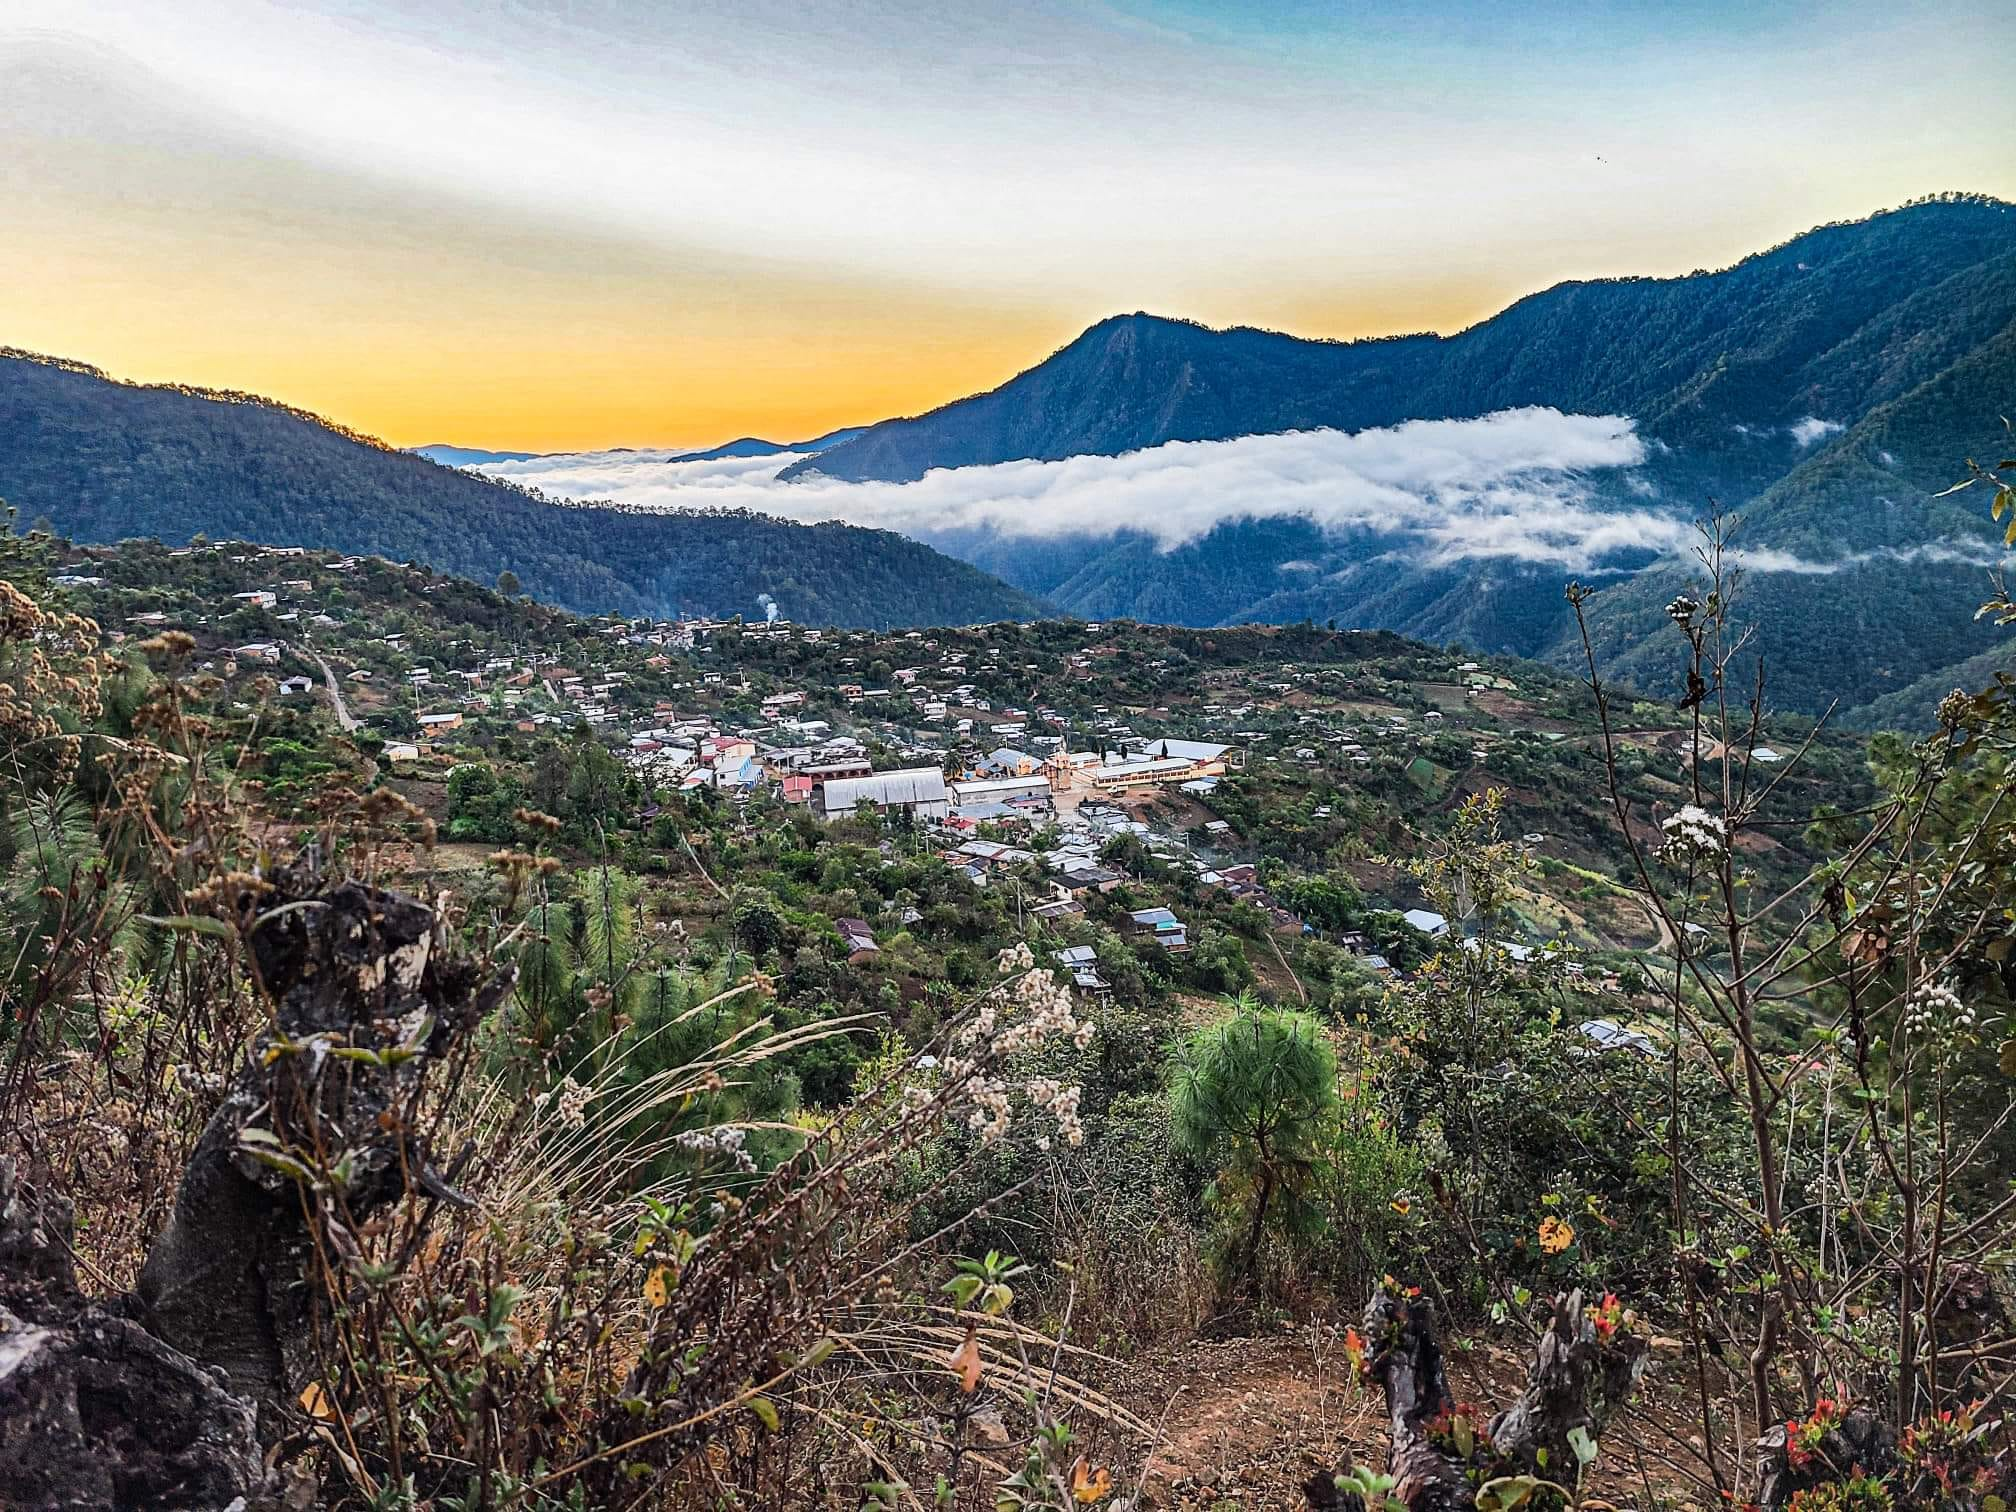
\includegraphics[width=0.9\textwidth]{images/SantiagoLaxopa.jpeg}
    \caption{Santiago Laxopa taken by Beto Diaz, a resident of Santiago Laxopa.}
    \label{fig:SantiagoLaxopa}
\end{figure}



%-------------------------
\section{Vowels in Santiago Laxopa Zapotec} \label{sec:SLZ-vowels}
%-------------------------

SLZ exhibits a four-vowel inventory; see Table~\ref{tab:SLZ_vowel_chart}. This type of vowel inventory is very common among Sierra Norte Zapotecs. Most varieties have the vowels /i/, /e/, /a/, and /o/ \citep{nellisFortisLenisCajonos1980,jaegerInitialConsonantClusters1982,butlerh.DiccionarioZapotecoYatzachi1997,avelinoTopicsYalalagZapotec2004,longDiccionarioZapotecoSan2005,sonnenscheinDescriptiveGrammarSan2005}. 

\begin{table}[h!]
    \centering
    \caption{Vowel qualities in Santiago Laxopa Zapotec.}
    \label{tab:SLZ_vowel_chart}
    \begin{tabular}{lccc}
        \lsptoprule
        &  front& central  & back \\
        \midrule
        high   	&  i  &     &   u$\thicksim$o \\
        mid    	&  e  &   	& 	\\
        low   	&     &  a 	&	  \\
        \lspbottomrule
    \end{tabular}
\end{table}

The vowel /o/ is marginal in SLZ's lexicon, only appearing in a few lexical items such as the diminutive classifier \textit{do'}. Instead, this vowel is replaced by /u/ in most cases. However, this difference is not universal among all speakers in the community. For the most part older speakers exhibit the vowel /o/ in their speech, while younger speakers tend to replace it with /u/. Most speakers, when asked, classify the two back rounded vowels as the same phoneme and view them as a dialectal feature between the different pueblos. For example, in neighboring San Bartolomé Zoogocho the /u/ vowel is very marginal and has led \citet{sonnenscheinDescriptiveGrammarSan2005} to describe the language as having only four vowels.It is interesting to note that everywhere that SLZ has the vowels /u/ or /o/, Zoogocho only has /o/. Further evidence for this comes from plotting the vowels along the first two formants. As shown in Figure~\ref{fig:SLZvowels}, the vowels /o/ and /u/ occupy nearly identical vowel spaces.

\begin{figure}[h!]
    \centering
    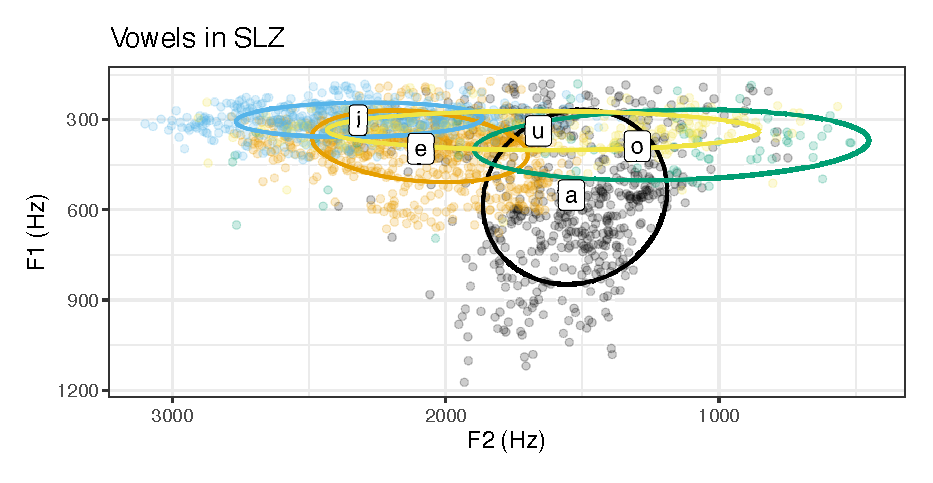
\includegraphics[width = 0.9\linewidth]{images/slz_vowels.eps}
    \caption{Vowel space of Santiago Laxopa Zapotec. The ellipses around each vowel mean represents 1 standard. The scale of the axes are in barks with their corresponding Hz values.}
    \label{fig:SLZvowels}
\end{figure}

Additional evidence for the overlap of /o/ and /u/ can be measured with a combination of Pillai scores \citep{pillaiNewTestCriteria1955,hayFactorsInfluencingSpeech2006,nyczBestPracticesMeasuring2014} and Bhattarcharyya's Affinity \citep{bhattacharyyaMeasureDivergenceTwo1943,johnsonQuantifyingOverlapBhattacharyyas2015,warrenQualityQuantityNew2018,strellufChapter3Low2018}. Both of these measures show what degree of overlap exists between two different items in some space. Their use in linguistics has been used mainly to show the process of complete and partial mergers between vowels, such as the \textsc{near-square} vowel merger in New Zealand English \citep{hayFactorsInfluencingSpeech2006}. The Pillai scores and Bhattacharyya's Affinity show that the vowels /o/ and /u/ are nearly identical in their vowel space; see Table~\ref{tab:SLZvowels_affinity}.

\begin{table}[!h]
    \centering
    \caption{Pillai scores and Bhattacharyya's Affinity for /o/ and /u/ in SLZ.}
    \label{tab:SLZvowels_affinity}
    \begin{tabular}{lcc}
        \lsptoprule
        &  Pillai score & Bhattacharyya's Affinity \\
        \midrule
        All speakers & 0.157 & 0.892 \\
        Females & 0.138 & 0.890 \\
        Males   & 0.224 & 0.858 \\
        \lspbottomrule
    \end{tabular}
\end{table}

In interpreting these results, Pillai scores range from 0 to 1, with 0 indicating overlap and 1 indicating complete no overlap. Bhattacharyya's Affinity ranges from 0 to 1, with 0 indicating no overlap and 1 indicating complete overlap. The results show that the overlap between /o/ and /u/ is not complete, but it is also not completely separating. This is consistent with the observations made by myself and other researchers for this variety (Toosarvandani, p.c.). 

In summary, we can conclude that SLZ is similar to other Northern Zapotec varieties in having a four-vowel inventory. The vowel /o/ is marginal in the lexicon and is often replaced by /u/ in younger speakers. The vowels /o/ and /u/ occupy nearly identical vowel spaces, and the overlap between the two vowels is not complete but is also not completely separating. 

%-------------------------
\section{Phonation in Santiago Laxopa Zapotec} \label{sec:SLZ-voicequality}
%-------------------------

One of the defining characteristics of the Oto-Manguean languages is their use of contrastive phonation \citep{campbellOtomangueanHistoricalLinguistics2017,campbellOtomangueanHistoricalLinguistics2017a}. This fact is so common and widespread that it is has been reconstructed for the proto-language (see \cite{renschComparativeOtomangueanPhonology1976}). Additionally, the use of contrastive phonation in Oto-Manguaean languages led \citet{silvermanLaryngealComplexityOtomanguean1997,silvermanPhasingRecoverability1997} to invent the term \textit{laryngeal complexity} to describe how phonation is realized in these languages and the development of theories of how phonation interacts with tone. 

Most Zapotec languages make use of contrastive phonation (see \cite{ariza-garciaPhonationTypesTones2018} for an overview and typology of the phonation contrasts in the Zapotec language family), with SLZ being no exception. SLZ
has a four-way voice quality contrast: modal, breathy, checked, and rearticulated. These contrasts are exemplified in the minimal quadruple in (\ref{ex:SLZphonation}).

\ea \label{ex:SLZphonation} Four-way near minimal phonation contrast
    \ea \textit{yag}  /çag\supr{L}/ `tree; wood; almúd (unit of measurement  $\thicksim$4kg)'
    \ex \textit{yah}  /ça̤\supr{L}/ `metal; rifle; bell'
    \ex \textit{cha'}  /tʃaˀ\supr{L}/  `cooking pot'
    \ex \textit{ya'a}  /çaˀa\supr{L}/  `market'
    \z
\z

%------------------------
\subsection{Breathy vowels in SLZ} \label{sec:SLZ-voicequality-breathy}
%------------------------
SLZ is also unique in regards to its voice quality contrasts because it is a Northern Core Zapotec that has developed breathy voice, which has not been described in any of the neighboring Sierra Norte varieties \citep{nellisFortisLenisCajonos1980,jaegerInitialConsonantClusters1982,butlerh.DiccionarioZapotecoYatzachi1997,avelinoTopicsYalalagZapotec2004,sonnenscheinDescriptiveGrammarSan2005,longDiccionarioZapotecoSan2005}.\footnote{Breathy voice in Zapotec languages, however, is common in Central Valley Zapotecs \citep{munroDicsyonaaryTeenDiizh1999,espositoSantaAnaValle2004,espositoVariationContrastivePhonation2010,uchiharaToneRegistrogenesisQuiavini2016,ariza-garciaPhonationTypesTones2018}.} Breathy voice is characterized by a raspiness throughout the whole vowel or a portion of the vowel depending on the speaker.

\begin{figure}[h!]
    \centering
    \includegraphics[width=0.9\textwidth]{images/Spectrograms/yah.png}
    \caption{Breathy vowel in the word \textit{yah} `metal; rifle'}
    \label{fig:BreathyVowel}
    
\end{figure}

%------------------------
\subsection{Checked vowels in SLZ} \label{sec:SLZ-voicequality-checked}
%------------------------
SLZ shares with most Zpaotec varities, two types of creaky voice: checked and rearticulated. Checked vowels are characterized by an abrupt glottal closure which cuts the vowel short. This phonation is sometimes realized as a period of creakiness at the end of the vowel.

\begin{figure}[h!]
    \centering
    % [INSERT YA SPECTROGRAM AND WAVEFORM]
    \includegraphics[width=0.9\textwidth]{images/Spectrograms/RD_yu'.png}
    \caption{Checked vowel in the word \textit{yu'} `earth'}
    \label{fig:CheckedVowel}
    
\end{figure}

%------------------------
\subsection{Rearticulated vowels in SLZ} \label{sec:SLZ-voicequality-rearticulated}
%------------------------
Among speakers of SLZ, there is a large amount of inter- and intra-speaker variability in how rearticulated vowels are produced. Some speakers produce these vowels with a full glottal stop in the middle of the vowel, others produce a vowel with apparent modal voice but with a drop in amplitude (similar to what \cite{gerfenProductionPerceptionLaryngealized2005} found for some Mixtec varities), while others produce creaky voice throughout the entire vowel. Some speakers produce a combination of these unique productions. Overall, these rearticulated vowels are proiduced with some form of manipulation of glottal closure or apmlitude drop in the middle of the vowel.

\begin{figure}[!h]
	\centering
	\begin{subfigure}{.5\textwidth}
		\centering
		\includegraphics[width=\linewidth]{Images/Spectrograms/za'a.png}
		\caption{\textit{za'a} `corncob'}
		\label{fig:FSRza'a}
	\end{subfigure}%
	\begin{subfigure}{.5\textwidth}
		\centering
		\includegraphics[width=\linewidth]{Images/Spectrograms/xa'ag.png}
		\caption{\textit{xa'ag} `topil'}
		\label{fig:FSRxa'ag}
	\end{subfigure}	
	\caption{FSR's rearticulated vowels in \textit{za'a} `corncob' and \textit{xa'ag} `topil'}
	\label{fig:FSRLaryngeal}
\end{figure}

\begin{figure}[!h]
	\centering
	\begin{subfigure}{.5\textwidth}
		\centering
		\includegraphics[width=\linewidth]{Images/Spectrograms/RD_za'a.png}
		\caption{\textit{za'a} `corncob'}
		\label{fig:RDza'a}
	\end{subfigure}%
	\begin{subfigure}{.5\textwidth}
		\centering
		\includegraphics[width=\linewidth]{Images/Spectrograms/RD_xa'ag.png}
		\caption{\textit{xa'ag} `topil'}
		\label{fig:RDxa'ag}
	\end{subfigure}
	\caption{RD's rearticulated vowels in \textit{za'a} `corncob' and \textit{xa'ag} `topil'}
	\label{fig:RDLaryngeal}
\end{figure}
%-------------------------
\section{Tonal contrasts in Santiago Laxopa Zapotec} \label{sec:SLZ-tones}
%-------------------------
One of the most well known features of all Oto-Manguean languages is the fact that they are tonal languages and exhibit a large range of tonal systems \citep{pikeProblemsZapotecTone1948,renschComparativeOtomangueanPhonology1976,josserandMixtecDialectHistory1983,silvermanLaryngealComplexityOtomanguean1997,beamdeazconaProblemsZapotecTone2007,dicanioItunyosoTrique2010,dicanioCoarticulationToneGlottal2012,elliottChicahuaxtlaTriqui2016,campbellOtomangueanHistoricalLinguistics2017,campbellOtomangueanHistoricalLinguistics2017a,lillehaugenOtomangueanLanguages2019,eischensTonePhonationPhonologyPhonetics2022}. SLZ has a five-way tonal contrast which consists of three level tones (high, mid, low) and two contour tones (rising and falling). 

\citet{brinkerhoffTonalPatternsTheir2022}

%------------------------------------
\section{Interactions between tone and voice quality} \label{sec:SLZ-interaction}
%------------------------------------

% Santiago Laxopa Zapotec (SLZ; \textit{Dilla'xhunh Laxup} [diʒaˀʐun laʂup]) is a Northern Zapotec language spoken by approximately 1000 people in the municipality of Santiago Laxopa, Ixtlán District in the Sierra Norte of Oaxaca, Mexico \citep{adlerAcousticsPhonationTypes2016,adlerDerivationVerbInitiality2018,foleyForbiddenCliticClusters2018,foleyExtendingPersonCaseConstraint2022}.\footnote{This macro variety is also sometimes called Cajonos Zapotec and comprises the dialects of Zoogocho Zapotec, Yatzachi Zapotec, Yalálag Zapotec, Tabaá Zapotec, and Lachirioag Zapotec \citep{smith-starkAlgunasIsoglosasZapotecas2003}.} It is mutually intelligible with San Bartolomé Zoogocho Zapotec \citep{longDiccionarioZapotecoSan2005,sonnenscheinDescriptiveGrammarSan2005}. SLZ has a fairly standard five-vowel inventory; see Table~\ref{tab:SLZvowels}.\footnote{The /o/ vowel is marginal in the lexicon for SLZ and only appears in a few lexical items. In neighboring San Bartolomé Zoogocho the /u/ vowel is very marginal and has led \citet{sonnenscheinDescriptiveGrammarSan2005} to describe the language as having only four vowels. It is interesting to note that everywhere that SLZ has the vowels /u/ or /o/, Zoogocho only has /o/. When plotting the vowel spaces and looking for outliers in the data based on F1 and F2, I noticed that the vowels /o/ and /u/ occupy nearly identical vowel spaces.}


		
% Among Zapotecan languages, it is quite common for languages to make use of contrastive phonation \citep[e.g.,][]{avelinoTopicsYalalagZapotec2004,longDiccionarioZapotecoSan2005,avelinoAcousticElectroglottographicAnalyses2010,lopeznicolasEstudiosFonologiaGramatica2016,chavez-peonInteractionMetricalStructure2010}. In \posscitet{ariza-garciaPhonationTypesTones2018} typological description of phonation in Zapotecan languages, most have two to three phonation types which are described as involving creaky phonation or a glottal closure that is considered a vocalic feature. \citet{ariza-garciaPhonationTypesTones2018} additionally notes that breathy phonation is quite rare among Zapotecan languages, with only three languages in her typological study having this phonation type. Based on this typological data, she claims that breathy phonation is a recent innovation and is restricted to the Valley Zapotec languages only. However, SLZ, as a Northern Zapotec language, presents evidence to the contrary. SLZ has a four-way phonation contrast: modal, breathy, checked, and laryngealized. These contrasts are exemplified in the minimal quadruple in (\ref{ex:YA}).
% \ea \label{ex:YA} Four-way near minimal phonation contrast
%     \ea \textit{yag}  /çag\supr{L}/ `tree; wood; almúd (unit of measurement approximately 4kg)'
%     \ex \textit{yah}  /ça̤\supr{L}/ `metal; rifle; bell'
%     \ex \textit{yu'}  /çuˀ\supr{L}/  `earth'
%     \ex \textit{ya'a}  /çaˀa\supr{L}/  `market'
%     \z 
% \z 

% In representing the checked and laryngealized vowels, I follow the same procedure as other authors (e.g., \citet{avelinoAcousticElectroglottographicAnalyses2010, uchiharaToneRegistrogenesisQuiavini2016}) in representing the ``glottal stop'' element as a superscript glottal stop in the IPA transcription (i.e., [aˀ] or [aˀa]). This is primarily done as a way of standardizing the variable pronunciation of the glottal element in Zapotec, ranging from a full glottal stop (i.e., [aʔ] or [aʔa]) to a creaky portion of the vowel (i.e., [aa̰] or [aa̰a ]).  
% Theoretically, one could argue that checked and laryngealized vowels are not actually phonation types but involve a glottal stop consonant, either as a syllabic onset or coda. It is indeed logical that this could be the case. However, much work has shown that this cannot be true in Zapotec for the laryngealized vowels, which have a glottal closure in their center. \citet{chavez-peonInteractionMetricalStructure2010} summarizes this work and offers six reasons why these ``glottal stops" are a vocalic feature, not a consonant in laryngealized vowels. The first reason has to do with the distribution of the glottal stop. If it is indeed a coda or onset, then we would expect it could also occur word-initially or in consonant clusters. This does not happen in SLZ or other Zapotec languages \citep{jaegerInitialConsonantClusters1982}. Another point that he raises is that when linguists ask native language consultants about how many syllables or beats the word has, they treat laryngealized vowels as if they only had a single beat.\footnote{This is something Maya Wax Cavallaro and I tested with one of our consultants. The only times that they said one of these laryngealized vowels was not a single beat was when they had differing vowel qualities on either side of the glottal closure (e.g., \textit{bi'a} [biˀa] `fly (insect)').} These and other points raised by \citeauthor{chavez-peonInteractionMetricalStructure2010} are presented in (2). 

% \ea  Summary: glottal stop as a vocalic feature in laryngealized vowels (adapted from \cite{chavez-peonInteractionMetricalStructure2010}).
%     \ea /ʔ/ defective distribution (not in onset, not in clusters)
%     \ex Larynealized vowels have the same tonal sequences as single vowels
%     \ex Monosyllabic tendency of the majority of languages (roots = 1σ)
%     \ex *VʔC\sub{fortis}, predicted by bimoraicity of laryngealized vowels
%     \ex Same vowel quality, i.e., one vowel gesture (diphthongs a minority)
%     \ex Perceived as single syllables by native speakers (ʔ ≠ sufficient consonantal barrier, i.e., syllable boundary)
%     \z 
% \z 

% One point that he doesn't mention is that if we assume the glottal stop is a coda consonant, then we would also expect to see the other phonation types being able to co-occur with this coda consonant. Much work still needs to be done from a phonological perspective. Treating /ʔ/ and /h/ as a vocalic feature or as a consonant is worth further study, but in the present work, I assume these sounds are vocalic features and contribute to the phonation contrasts following the traditional interpretation of these sounds. 

% Breathy vowels in SLZ are characterized by a raspiness throughout the whole vowel or a portion of the vowel; see Figure~\ref{fig:BreathyVowel}. For some speakers, it appears as if the breathiness is aligned with the beginning of the vowel and others have it aligned to the end of the vowel. 

% \begin{figure}[!h]
% 	\centering
% 	% [INSERT YAH SPECTROGRAM AND WAVEFORM]
% 	\includegraphics[width=0.9\textwidth]{Images/yah.png}
% 	\caption{Breathy vowel in the word \textit{yah} `metal; rifle'}
% 	\label{fig:BreathyVowel}
% \end{figure}

% On the other hand, checked vowels are characterized by an abrupt glottal closure which cuts the vowel short. This phonation is sometimes realized as a period of creakiness at the end of the vowel; see Figure~\ref{fig:CheckedVowel}.  

% \begin{figure}[!h]
% 	\centering
% 	% [INSERT YA SPECTROGRAM AND WAVEFORM]
% 	\includegraphics[width=0.9\textwidth]{Images/RD_yu'.png}
% 	\caption{Checked vowel in the word \textit{yu'} `earth'}
% 	\label{fig:CheckedVowel}
% \end{figure}

% Laryngealized vowels are common in Zapotecan languages and have received many names. Previous descriptions have used terms such as broken, rearticulated, interrupted, and creaky to describe this phonation type \citep{longDiccionarioZapotecoSan2005,avelinoTopicsYalalagZapotec2004,avelinoAcousticElectroglottographicAnalyses2010,sonnenscheinDescriptiveGrammarSan2005,adlerAcousticsPhonationTypes2016}. To avoid confusion; I will use the term laryngealized following \citet{avelinoAcousticElectroglottographicAnalyses2010}. In addition to their many different names, these vowels exhibit a wide range of allophones. 

% \citet{avelinoAcousticElectroglottographicAnalyses2010} found in the closely related Yalálag Zapotec that among his consultants, there were at least four different pronunciations as seen in Table~\ref{tab:laryngeal}. 
% \begin{table}[!h]
% 	\centering
% 	\caption{Layngealized Vowels in Yalálag Zapotec}
% 	\label{tab:laryngeal}
% 	 \begin{tabular}{ll}
% 	\lsptoprule
% 	/VˀV/	&  [VʔV]  \\
% 			&  [VV̰V]   \\
% 			&  [VV̰ːV̆]  \\
% 			&  [VV̰V̰]	\\
% 	\lspbottomrule
% 	\end{tabular}
% \end{table}

% In SLZ, this vowel is also highly variable. For most speakers, laryngealized vowels were either creaky throughout their entire production or had a period of creakiness in the middle of the vowel. However, there is a large amount of inter- and intra-speaker variability in how this sound is produced. Some of these other productions included producing modal voice throughout, except for a short period of two or three glottal pulses, which showed a drop in amplitude of five to ten decibels. This drop in amplitude is not too surprising as \citet{gerfenProductionPerceptionLaryngealized2005} showed that this drop in amplitude was sufficient to cue these laryngealized vowels in Coatzospan Mixtec, a member of the Amuzgo-Mixtecan branch of the Oto-Manguean language family. Another frequent production was a complete glottal closure in the middle of the vowel producing a true re-articulation of the vowel. In addition to these productions, combinations of these unique productions were also encountered. Based on my observations, these differences cannot be attributed to sociolinguistic factors (e.g., age, sex, gender, socio-economic status) but seem to be in free variation. 

% To showcase some of these production differences, I show the production of two SLZ speakers who live in Santa Cruz, CA, who participated in piloting this study before I went to Santiago Laxopa for data collection. One of the SLZ speakers in Santa Cruz would re-articulate with a full glottal stop in the middle of the vowel or produce creaky voice. This alternation seemed to be in free variation. Still, there was a greater tendency to creak in low-toned words, such as \textit{xa'ag} [ʂa̰ːg] `topil'\footnote{A \textit{topil} is a type of government office in traditional Oaxacan communities somewhat akin to a sheriff.}, and re-articulate elsewhere; see Figure~\ref{fig:FSRLaryngeal}.

% \begin{figure}[!h]
% 	\centering
% 	\begin{subfigure}{.5\textwidth}
% 		\centering
% 		\includegraphics[width=\linewidth]{Images/za'a.png}
% 		\caption{\textit{za'a} `corncob'}
% 		\label{fig:FSRza'a}
% 	\end{subfigure}%
% 	\begin{subfigure}{.5\textwidth}
% 		\centering
% 		\includegraphics[width=\linewidth]{Images/xa'ag.png}
% 		\caption{\textit{xa'ag} `topil'}
% 		\label{fig:FSRxa'ag}
% 	\end{subfigure}	
% 	\caption{Comparison of FSR's laryngealized vowels in \textit{za'a} `corncob' and \textit{xa'ag} `topil'}
% 	\label{fig:FSRLaryngeal}
% \end{figure}

% The other SLZ speaker only produces creaky voice for these vowels regardless of the tone of the word. During one of the elicitation sessions, my fellow researchers and I conducted a perceptual check that these were, in fact, the same vowels. Both consultants reliably identified the words. They produced laryngealized vowels according to their own idiosyncrasies.
% \begin{figure}[!h]
% 	\centering
% 	\begin{subfigure}{.5\textwidth}
% 		\centering
% 		\includegraphics[width=\linewidth]{Images/RD_za'a.png}
% 		\caption{\textit{za'a} `corncob'}
% 		\label{fig:RDza'a}
% 	\end{subfigure}%
% 	\begin{subfigure}{.5\textwidth}
% 		\centering
% 		\includegraphics[width=\linewidth]{Images/RD_xa'ag.png}
% 		\caption{\textit{xa'ag} `topil'}
% 		\label{fig:RDxa'ag}
% 	\end{subfigure}
% 	\caption{Comparison of RD's laryngealized vowels in \textit{za'a} `corncob' and \textit{xa'ag} `topil'}
% 	\label{fig:RDLaryngeal}
% \end{figure}

% %------------------------------------
% \subsection{Interaction of Tone and Phonation} \label{sec:Interaction}
% %------------------------------------

% Most previous work on the interaction of tone and phonation has been focused on the languages of East and Southeast Asia (e.g., \cite{masicaDefiningLinguisticArea1976,thurgoodVietnameseTonogenesisRevising2002,yipTone2002,enfieldArealLinguisticsMainland2005,michaudComplexTonesEast2012,brunelleTonePhonationSoutheast2016}). What has been found in these descriptions is that certain tones and phonations are codependent. For example, \citet{smalleyProblemsConsonantsTone1976} and \citet{ratliffMeaningfulToneStudy1992} both describe White Hmong's \textit{-g} tone as being a mid-low tone with breathy phonation, and Mandarin's tone 3 is often associated with creaky phonation \citep{hockettPeipingPhonology1947}. \citet{brunelleTonePerceptionNorthern2009} found that creaky phonation plays an important role in producing certain tones. Additionally, work on S'gaw Karen has found that two tones are only differentiated by some form of non-modal phonation (Boehm p.c.). 

% However, there have been some observations–especially in Mesoamerica–that tone and phonation are independent of each other \citep[e.g.,][]{silvermanLaryngealComplexityOtomanguean1997,garellekAcousticConsequencesPhonation2011}. This means that tone can independently occur with any phonation type. This has also been extensively described in multiple Zapotecan languages \citep[e.g.,][]{,avelinoTopicsYalalagZapotec2004,avelinoAcousticElectroglottographicAnalyses2010, chavez-peonInteractionMetricalStructure2010, campbellZenzontepecChatinoAspect2011,villardPhonologyMorphologyZacatepec2015, lopeznicolasEstudiosFonologiaGramatica2016}

% \citet{chavez-peonInteractionMetricalStructure2010} describes the tone and phonation interactions in San Lucas Quiaviní Zapotec (SLQZ), a central valley variety of Zapotec. The distribution of tone and phonation is found in Table~\ref{tab:SLQZ}. We see that in SLQZ, both low- and falling-tones have the full range of possible combinations. However, we see gaps in the high-tone for breathy and rising tones that can only occur with modal phonation. 

% \begin{table}[h!]
% 	\centering
% 	\caption{SLQZ tone and phonation interactions \citep{chavez-peonInteractionMetricalStructure2010}.}
% 	\label{tab:SLQZ}
% 	 \begin{tabular}{lcccc}
% 	  \lsptoprule
% 					  &	 \textbf{Modal}  & \textbf{Breathy} & \textbf{Creaky} & \textbf{Interrupted} \\
% 		  High	& ✔︎ & -- & ✔︎ & ✔︎ \\
% 		  Low & ✔︎ & ✔︎ & ✔︎ & ✔︎ \\
% 		  Falling & ✔︎ & ✔︎ & ✔︎ & ✔︎ \\
% 		  Rising & ✔︎ & -- & -- & -- \\
% 	  \lspbottomrule
% 	 \end{tabular}
% \end{table}

Based on elicitation data collected from 2020-2022, SLZ has a more expansive distribution of tone and phonation when compared to SLQZ but seems to be very similar to other Northern Zapotec varieties \citep[e.g.,][]{avelinoTopicsYalalagZapotec2004}. The distribution of SLZ tonal and phonation combinations are given in Table~\ref{tab:ToneVoiceQuality}.
\begin{table}[!h]
	\caption{SLZ tone and voice quality combinations.}
	\label{tab:ToneVoiceQuality}
	\centering

	\begin{tabular}{lcccc}
	\lsptoprule
		& \textbf{Modal} & \textbf{Breathy} & \textbf{Checked} & \textbf{Rearticulated} \\
	\hline
	High		& ✔︎ & -- & ✔︎ & ✔︎ \\
	Mid			& ✔︎ & ✔︎ & ✔︎ & ✔︎ \\
	Low			& ✔︎ & ✔︎ & ✔︎ & ✔︎ \\
	High-Low	& ✔︎ & ✔︎ & ✔︎ & ✔︎ \\
	Mid-High	& ✔︎	& ✔︎ & -- & ✔︎ \\
	\lspbottomrule
	\end{tabular}
\end{table}

% One of the striking things in this is the lack of high tone with breathy phonation. This gap is interesting because of the long-time association of high pitch with breathiness \citep[a good overview–of this association and other phonation types–is found in][]{eslingVoiceQualityLaryngeal2019}. This gap is common across the Zapotecan languages that have breathy voice (Campbell p.c.). Regarding breathy phonation in SLQZ, one of the Valley Zapotec varieties, \citet{uchiharaToneRegistrogenesisQuiavini2016} offers some convincing evidence that the phonation originated in syllables with low tone and then spread to other tones via analogy. Investigating the origin of breathy voice in SLZ would be important in understanding how breathy vowels originated in the Zapotecan family where breathy voice is rare typologically \citep{ariza-garciaPhonationTypesTones2018}. Such a study is beyond the scope of this paper.  
% Description: This file contains the content of the chapter 3 of the dissertation. It is based on an article that me and Grant wrote.

%------------------------------------------------
\chapter{On using Residual H1* for voice quality research} \label{ch:residual_h1}
%------------------------------------------------
%------------------------------------------------
\section{Introduction} \label{sec:Intro}
%------------------------------------------------

Languages use voice quality distinctions to convey phonemic distinctions \citep{garellekPhoneticsVoice2019} and to convey paralinguistic information by ``indexing the biological, psychological, and social characteristics of the speaker" \citep{laverVoiceQualityIndexical1968,podesvaStanceWindowLanguageRace2016}. Voice quality contrasts have been studied extensively by examining their correlates in the acoustic signal \citep[e.g.,][]{espositoCrosslinguisticPatternsPhonation2020}, resulting in a large and complex literature on acoustic correlates of phonation differences \citep[see][]{garellekPhoneticsVoice2019}. 

One measure that Fischer-Jorgensen established, the fundamental's relative strengthive amplitudes of the first harmonic and second harmonic. As established by Fischer-Jorgensen, the relative strength of the fundamental is a correlated measure of breathy voice in contrast with modal voice \citet{fischer-jorgensenPhoneticAnalysisBreathy1968}. In order to normalize the amplitude of the fundamental and counteract some of the effects of high-pass filtering and differences in sound pressure in the signal, she proposed that you could subtract the amplitude of a higher harmonic, in this case, the second harmonic (H2), from the amplitude of the fundamental (H1). Since its introduction, H1*$-$H2* has been used in many studies to measure not only breathy voice but other voice quality contrasts as well \citep{garellekPhoneticsVoice2019,chaiH1H2AcousticMeasure2022}.

Despite the large amount of evidence in support of H1*$-$H2*, it is not without its problems. At the fundamental level, it is not clear that H1*$-$H2* adequately measures the strength of the fundamental. \citet{sundbergObjectiveCharacterizationPhonation2022} found that H1 and H2 are affected differently by subglottal pressure, compromising some of the original reasoning behind the use of H1*$-$H2* from \citet{fischer-jorgensenPhoneticAnalysisBreathy1968}. Similarly, in a comprehensive overview of the main concerns with H1*$-$H2* as a phonation type measure, \citet{chaiH1H2AcousticMeasure2022} found that in addition to the issues mentioned above, errors in measuring H1*$-$H2* are uncomfortably high. This is mainly due to the need to precisely measure two different harmonic amplitudes; when there are errors in calculating H1, this, in turn, leads to errors in calculating H2 \citep{arrasIntroductionErrorPropagation1998}. An example of this type of error propagation is that errors in measuring the fundamental frequency, which is especially common with non-modal phonation, are introduced into measuring harmonics because they are based on the fundamental. Despite algorithms correcting for vowel height, a common error that occurs is when a high fundamental frequency co-occurs with a low first formant \citep{chaiH1H2AcousticMeasure2022}. This situation causes errors in tracking the fundamental frequency and the first formant. A final issue that can occur when measuring the harmonics is in contexts where the vowel is nasalized. \citet{simpsonFirstSecondHarmonics2012} shows that in these nasalized contexts, the first nasal pole (P0) can increase the amplitude of H2 and, when the fundamental frequency is high, H1 increases instead.

This collection of errors leads \citet{chaiH1H2AcousticMeasure2022} to propose a new measure, residual H1*. This measure is calculated by first regressing H1 on energy and then subtracting the product of energy and the energy factor from H1. Chai and Garellek argue that this measure better reflects the initial purpose of using H1*$-$H2*. Furthermore, they find that residual H1*: (i) provides better differentiation between phonation types in !Xóõ; (ii) was more robust for measuring creak in Mandarin with respect to different utterance positions; and (iii) has a stronger relationship to the open quotient than H1*H2* based on a comparison using electroglottogram data.

The contributions \citet{chaiH1H2AcousticMeasure2022} make are very intriguing and have the potential to alter how spectral analyses of voice quality are performed. However, they are not convincing on their own. If residual H1* is to be widely adopted in linguistics, speech pathology, and other speech sciences, then it requires considerable evidence of its effectiveness in acoustic studies. This paper offers additional evidence for residual H1*'s effectiveness. 

Given the promising nature of this measure, we tested residual H1* with data from Santiago Laxopa Zapotec. Although \citet{chaiH1H2AcousticMeasure2022} evaluated residual H1* for !Xóõ and Mandarin, both of which contain tone and voice quality, they do not factor tone into their analysis.\footnote{!Xóõ is most like Zapotec in that it has three phonologized phonation categories. It also has tone, which to our understanding is not restricted by phonation and which is not analyzed in \citet{chaiH1H2AcousticMeasure2022}. The Mandarin case is less relevant as its phonation is prosodic and tonally linked.} This is where testing the effectiveness of residual H1* in Zapotec languages is beneficial. Zapotec languages are often described as laryngeally complex \citep{silvermanLaryngealComplexityOtomanguean1997,ariza-garciaPhonationTypesTones2018}. Laryngeal complexity is defined as a language that allows contrastive tone and contrastive voice quality that are unrestricted in their interactions. This laryngeal complexity between tone and phonation types presents a unique challenge for acoustic analysis and testing of the residual H1* measure. 

Other Zapotec languages have also been studied for voice quality research. For example, \citet{espositoVariationContrastivePhonation2010} found that in Santa Ana del Valle Zapotec there was a biological sex difference in which acoustic measures best capture the voice quality contrasts similar to observations from \citet{klattAnalysisSynthesisPerception1990}. \citet{arellanesarellanesDosGradosLaringizacion2010} found that the realization of laryngealization in a variety of San Pablo Güilá Zapotec is highly variable and depends on the position of laryngealization in the phrase. This was also found to be the case in Betaza Zapotec \citep{crowhurstInfluenceVowelLaryngealisation2016}. \citet{barzilaiContextdependentPhoneticEnhancement2021} found that tone and phrasal position also played a role in how voice quality is realized in San Pablo Macuiltianguis Zapotec. These studies show that Zapotec languages have much to contribute to our understanding of voice quality. 

We find that residual H1* can adequately capture differences in voice quality and is a more robust measure of voice quality than H1*$-$H2*, adding credence to the use of this measure instead of H1*$-$H2* in voice quality research. The remainder of this paper is organized as follows. Section~\ref{sec:SLZ} provides a brief overview of the Santiago Laxopa Zapotec language. Section~\ref{sec:Methods} describes the methods used in the data collection, data processing, and statistical modeling used in this study. Section~\ref{sec:Results} presents the results of the study. Section~\ref{sec:Conclusion} concludes the paper.

%----------------------------------------------------------------------------------------
\section{Santiago Laxopa Zapotec} \label{sec:SLZ}
%----------------------------------------------------------------------------------------
Santiago Laxopa Zapotec is a Northern Zapotec language of the Oto-Manguean language family \citep{adlerAcousticsPhonationTypes2016,adlerDerivationVerbInitiality2018,foleyForbiddenCliticClusters2018,foleyExtendingPersonCaseConstraint2022,sichelPronounsAttractionSierra2020,
sichelFeaturalLifeNominals2020,brinkerhoffDownstepSantiagoLaxopa2021,brinkerhoffTonalPatternsTheir2022}. It is spoken by 981 people in the municipality of Santiago Laxopa, Ixtlán, Oaxaca, Mexico and a small number of other speakers from the diaspora in Mexico and the United States. 

Santiago Laxopa Zapotec exhibits a four-vowel inventory (that is, /i/, /e/, /a/, and /u/), which is further distinguished by a four-way contrast in voice quality. This variety is unique because it is a Northern Zapotec that has developed a breathy voice (/V̤/) in addition to the two types of laryngealization that characterize the rest of the Zapotec languages, namely checked and articulated. Checked vowels are defined as a modal vowel that ends with a period of creaky voice or a glottal closure (/VV̰/ or /Vˀ/ ). Rearticulated vowels are also defined as a modal vowel that also has a period of creakiness or glottal closure but aligned to the middle of a vowel (/VV̰V/ or /VˀV/). This makes an otherwise modal vowel appear as if it is interrupted by this laryngealization.\footnote{This is different from how rearticulated vowels are defined in other languages, where they are a modal vowel followed by an ``echo vowel" which may or may not have a glottal closure intervening between the modal and ``echo" vowel \citep[see][]{bairdPhoneticPhonologicalRealizations2011}. A fuller description of how these vowels are realized in one variety of Zapotec and the terms used are found in \citet{avelinoAcousticElectroglottographicAnalyses2010}.} This difference in laryngeal timing is one of the key differences between these phonations (see \cite{ariza-garciaPhonationTypesTones2018} for a detailed typological study of voice quality distinctions in Zapotec languages).

Santiago Laxopa Zapotec is also tonal with three level tones (H, M, and L) and two contours (MH and HL) appearing in nominals \citep{brinkerhoffTonalPatternsTheir2022}.\footnote{The tonal system of Santiago Laxopa Zapotec for verbs and other lexical categories is still being evaluated.} The language has a complex interaction between tone and phonation types. Every tone can appear with every phonation type, with two exceptions being that breathy voice cannot appear with the high tone and checked voice cannot appear with the rising contour tone. It is unclear whether these are accidental gaps or have a phonetic underpinning.

These interactions between voice quality and tone present a rich environment for testing the reliability of voice quality measures in laryngeally complex languages.

\section{Methods} \label{sec:Methods}
\subsection{Elicitation} \label{sec:Elicitation}

Ten native speakers of SLZ (five female; five male) participated in a wordlist elicitation. Elicitation was performed in the pueblo of Santiago Laxopa, Ixtlán, Oaxaca, Mexico during the summer of 2022 using the built-in microphone of a Zoom H4n handheld recorder (16-bit, 44.5 kHz). 

The wordlist consisted of 72 items repeated three times in isolation and the carrier sentence \textit{Shnia' X chonhe lhas} [ʃnːiaˀ X tʃone ɾas] ``I say X three times''. This sentence was chosen to minimize any effect of the phrasal position \citep[see][for a study about phrasal effects on voice quality in Zapotec]{crowhurstInfluenceVowelLaryngealisation2016}. Additionally, there are no co-articulatory effects on voice quality found with this frame and the items in the wordlist.  Between these 72 words, there were 11 words with breathy voice, 9 with rearticulated voice, 10 with checked voice, and 42 with modal. Thirteen of the 72 words were disyllabic and eight of the thirteen contained the same voice quality in each syllable. Of those 13 disyllabic word, only five contained different voice qualities in each of the syllables. This resulted in 85 different syllables.\footnote{There is ongoing debate about the status of strong syllables in Zapotec. The majority of evidence for the presence of stress comes from non-Northern Zapotec varieties \citep[e.g.,][]{chavez-peonPhoneticCuesStress2008,mockPitchAccentStress1988}. At this time, evidence for stress in Northern Zapotec remains to be seen.} 

The token selection for the wordlist was done in consultation with a native speaker. Similarly to \citet{barzilaiContextdependentPhoneticEnhancement2021}, we did not balance the tones with the different voice qualities. The frequency in which certain tones co-occur with certain voice qualities is uneven in the language, making it difficult to control for. The distribution of tones and voice quality across the 85 syllables used in this study are presented in Table~\ref{tab:distribution}. This imbalance was taken into account by including Tone as a fixed effect in our statistical models in Section~\ref{sec:StatisticalModeling}.

\begin{table}[!h]
  \centering
  \caption{Distribution of tone and voice quality in the wordlist}
  \label{tab:distribution}
    \begin{tabular}{llllll}
    \lsptoprule
    & High & Mid & Low & Rising & Falling\\
    \hline
    Modal & 14 & 9 & 15 & 2 & 10 \\
    Breathy & $-$ & $-$ & 11 & $-$ & 2 \\
    Checked & 1 & $-$ & 9 & $-$ & \\
    Rearticulated & 1 & $-$ & 4 & $-$ & 4 \\
    \lspbottomrule
    \end{tabular}
\end{table}


%----------------------------------------------------------------------------------------
\subsection{Data Processing} \label{sec:DataProcessing}
%----------------------------------------------------------------------------------------

Each vowel of the target words in the carrier sentence condition was labeled following \citet{garellekAcousticDiscriminabilityComplex2020} for where the vowel began and ended. Each vowel in the word list was annotated for speaker, word, vowel, tone, voice quality, and utterance number. This labeling was conducted for each vowel in the target word from the elicitation list of the carrier sentences.

These vowels were then extracted and fed into VoiceSauce for acoustic measurement \citep{shueVoiceSauceProgramVoice2011}. The formants were measured using Snack \citep{sjolanderSnackSoundToolkit2004}, while the fundamental frequency (\textit{f0}) was measured using the STRAIGHT algorithm \citep{kawaharaInstantaneousfrequencybasedPitchExtraction1998}. Spectral slope measures were corrected for formants and bandwidths \citep{hansonGlottalCharacteristicsFemale1997,iseliAgeSexVowel2007}. Each vowel was measured with ten equal time intervals, resulting in 22890 data points in total.

The data were cleaned of outliers following the same steps as taken by \citet{chaiH1H2AcousticMeasure2022} in their study. The H1*, H1*–H2*, and \textit{f0} values were z-scored by speaker to reduce the variation between the speakers and provide a way to directly compare the different measures on the same scale. Data points with an absolute z-score value greater than 3 were considered outliers and excluded from the analyses. Within each vowel category, we calculated the Mahalanobis distance in the F1-F2 panel. Each data point with a Mahalanobis distance greater than 6 was considered an outlier and excluded from the analysis. Using the Mahalanobis distance allows us to compare the data points to the mean of the F1-F2 panel for each vowel category. The larger the Mahalanobis distance is the more deviant the data point is from the mean which in turn means that the data point was improperly tracked. This is comparable to what was done in \citet{seyfarthPlosiveVoicingAcoustics2018,chaiCheckedSyllablesChecked2022,garellekPhoneticsWhiteHmong2023}.

Time points whose \textit{f}0, F1, or F2 values were outliers were also excluded from H1* and H1*$-$H2* analyzes because H1* and H1*$-$H2* are calculated based on \textit{f0}, F1, and F2. Energy was excluded if it had a zero value and then logarithmically transformed to normalize its right-skewed distribution. Afterward, the resulting logarithmically transformed data was z-scored, and any data point with a z-score greater than 3 was excluded. This outlier removal resulted in 1918 datapoints being removed. 

After removing the outliers, we calculated residual H1* for the remaining data points following \citet{chaiH1H2AcousticMeasure2022}. First, a linear mixed effects model was generated with the z-scored H1* as the response variable and the z-scored energy as the fixed effect. The uncorrelated interaction of the z-scored energy by speaker was treated as random. The energy factor resulting from this linear mixed-effects model was extracted. Finally, the z-scored H1* had the product of the z-scored energy and the energy factor subtracted from it, giving us the residual H1* measure.

The measures were then orthogonally coded according to their position in the vowel (first, middle, and third) and for tone (H, M, L, R, F) for statistical modeling.  

%----------------------------------------------------------------------------------------
\subsection{Statistical modeling} \label{sec:StatisticalModeling}
%----------------------------------------------------------------------------------------

Two linear mixed-effects regression models were fitted, one for the normalized H1*$-$H2* and residual H1*. Each model had the tone and the interaction between voice quality and position in the vowel as fixed effects. Vowel and interaction between the speaker, the word, and the repetition were treated as random intercepts.\footnote{ $Measure \sim  Phonation*Position + Tone + (1|Speaker:Word:Repetition) + (1|Vowel)$}

The tone and the interaction between voice quality and position in the vowel were selected as fixed effects for several reasons. The first is that five unique tones appeared in the data and it is well established that tone interacts with voice quality in different ways (see \cite{espositoCrosslinguisticPatternsPhonation2020} and \cite{garellekPhoneticsVoice2019} for discussion). By treating tone as a fixed effect in our model, we can account for these interactions. The interaction between voice quality and position in the vowel as a fixed effect was included to account for the temporal differences between the two different laryngealizations, checked and rearticulated vowels. Checked vowels in Zapotec languages have a glottal occlusion or a short period of creaky voice located at the right edge of the vowel. This is in contrast to rearticulated vowels, where there is a glottal occlusion or creaky voice in the middle of the vowel. Because this difference between checked and rearticulated vowels is temporal in nature, we can account for this difference through the interaction of voice quality and position in the vowel.\footnote{Tone and voice quality are closely linked. By including only the positional interaction with voice quality, we can avoid collinear interactions that appear when we try to include tone in the interaction.}

The interaction between speaker, word, and repetition was treated as a random intercept because this allows us to consider that each speaker said each word on the elicitation list three times. This intercept accounts for not only the intra-speaker variability, but also the inter-speaker variability during each time the word was uttered. Treating a vowel as a random intercept allows us to capture the fact that each voice quality occurred with different vowels during elicitation.

Additional statistical modeling was performed with two generalized additive mixed models (GAMM) using the \texttt{mgcv} package in R \citep{woodGeneralizedAdditiveModels2017}. The GAMMs were fitted to account for any non-linear effects that may be present in the data. In each case the response variable was the same as in the linear mixed-effects models with voice quality as a fixed effect. Splines where used to model the non-linear effects of position and position by phonation. Speaker and word were treated as random intercepts.

%---------------------------------------------------------------------
\section{Results} \label{sec:Results}
%---------------------------------------------------------------------

In interpreting the results, there are certain expectations about how these measures should capture the voice quality contrasts. As discussed in \citet{garellekPhoneticsVoice2019}, it is expected that breathy vowels should have a higher spectral slope than modal vowels across the two measures in keeping with observations about breathy vowels in other languages. Because both checked and rearticulated vowels make use of creaky voice, they should have a lower spectral slope than modal vowels. Additionally, because there is a temporal distinction between checked and rearticulated with where the creakiness appears, this should also be captured in the two measures. 

%---------------------------------------------------------------------
\subsection{\texorpdfstring{H1*$-$H2*}{H1*-H2*}} \label{sec:H1H2}
%---------------------------------------------------------------------

Figure~\ref{fig:FIG1} shows the mean H1*$-$H2* values for each voice quality at each of the ten vowel intervals. We see that the breathy, checked, and rearticulated values are lower than the modal values at each of the first nine intervals. In the final intervals, breathy and rearticulated are essentially equal to the modal value. In contrast, checked's value remains lower than the modal's value throughout the entire vowel. This measure does not match the expectations discussed above.

\begin{figure}[htbp]
  \centering
  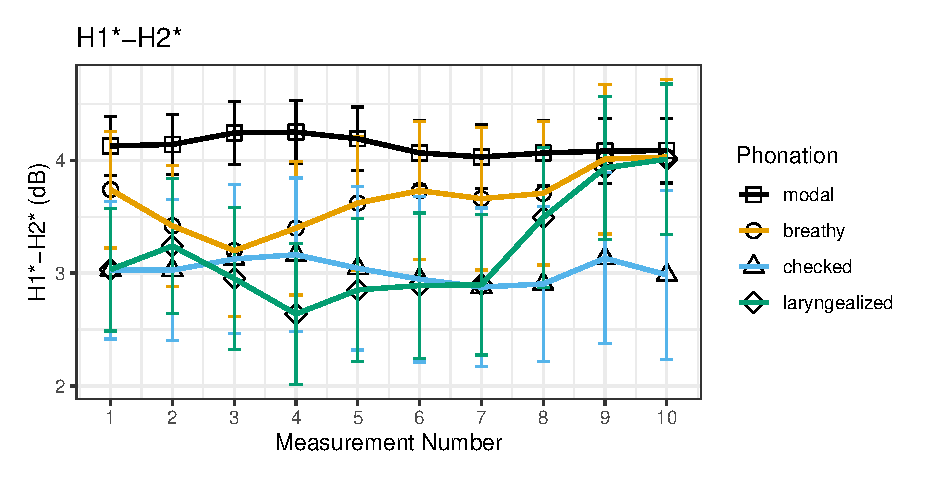
\includegraphics[width = 0.75\textwidth]{images/Figure1.eps}
  \caption{\label{fig:FIG1}{H1*$-$H2* across the duration of the vowel. Points represent the mean of each measure across the ten intervals. The error bars around each point represent a 95\% confidence interval. A line was plotted over each to show how the acoustic measure functions across the ten intervals.}}
\end{figure}

%----------------------------------------------------------------------------------------
\subsection{Residual H1*} \label{sec:ResidH1}
%----------------------------------------------------------------------------------------

Figure~\ref{fig:FIG2} shows the mean residual H1* values for each voice quality at each of the ten vowel intervals. In contrast to Figure~\ref{fig:FIG1}, we see that breathy has a higher residual H1* measure than modal throughout the duration of the vowel, which is consistent with other observations for breathy voice \citep{fischer-jorgensenPhoneticAnalysisBreathy1968}. Checked and rearticulated both have lower values than the modal at each of the 10 intervals. In addition, it shows that the checked voice has a lower residual H1 * value than the rearticulated voice at intervals 8 through 10. The rearticulated voice has a lower residual H1 * value than the checked voice at intervals 1 through 7, showing the temporal distinction between these two voice qualities. This measure complies with the expectations discussed above. 

\begin{figure}[htbp]
  \centering
  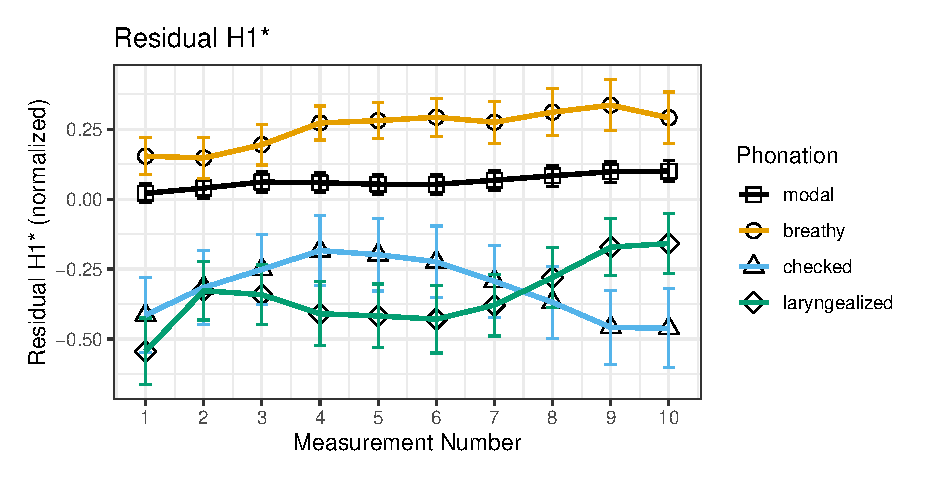
\includegraphics[width = 0.75\textwidth]{images/Figure2.eps}
  \caption{\label{fig:FIG2}{Residual H1* across the duration of the vowel. Points represent the mean of each measure across the ten intervals. The error bars around each point represent a 95\% confidence interval. A line was plotted over each to show how the acoustic measure functions across the ten intervals.}}
\end{figure}


%----------------------------------------------------------------------------------------
\subsection{Model Comparison} \label{sec:Comparison}
%----------------------------------------------------------------------------------------

To assess the robustness of the models, we compared the residual H1* linear mixed-effects model to the H1*$-$H2* linear mixed-effects model. This was done using two methods: direct comparison of the outputs of the two models in the same way as \citet{chaiH1H2AcousticMeasure2022} and the Akaike Information Criterion (AIC). 

Table~\ref{tab:CGComparison} compares the linear mixed effects models for H1*$-$H2* and residual H1*. In comparing these models, we find that the residual H1* model performed better than the H1*$-$H2* model in distinguishing voice quality contrasts in Santiago Laxopa Zapotec. This is supported by the larger absolute value of the coefficient estimate, the lower standard error, and the higher t-value of the residual H1* to distinguish breathy, checked, and rearticulated vowels from modal vowels.

\begin{table}[!h]
  \centering
  \caption{Model comparison between H1*$–$H2* and Residual H1* in distinguishing Santiago Laxopa Zapotec voice quality.}
  \label{tab:CGComparison}
    \begin{tabular}{lllllll}
      \lsptoprule
    Voice Quality Contrast & Model & \textit{$\beta$ } & Std. Error & \textit{t}-value & \textit{p}-value  &     \\
    \hline
      Breathy vs Modal &  H1*$-$H2* & 0.04631 & 0.03806  & 1.21680 & 0.22372 & \\
      & Res. H1* & 0.23625 & 0.02866 & 8.24177   & \textless 0.001   & *** \\
      Checked vs Modal & H1*$-$H2* & -0.11880 & 0.03476 & -3.41793  & \textless 0.001 & *** \\
      & Res. H1* & -0.40099 & 0.02621 & -15.30098 & \textless 0.001 & *** \\
      Rearticulated vs Modal & H1*-H2 & -0.09175 & 0.04588 & -1.99968 & 0.04560 & *  \\
     & Res. H1* & -0.44162 & 0.03450 & -12.80027 & \textless 0.001 & *** \\
     \lspbottomrule
    \end{tabular}
\end{table}

Table~\ref{tab:Comparison} shows the results of the AIC comparison between the H1*$-$H2* and residual H1* models. The residual H1* model had a lower AIC than the H1*$-$H2* model, indicating that the residual H1* model is a better fit for the data than the H1*$-$H2* model. Although AIC comparison is usually performed on nested models, it is still a useful tool for comparing non-nested models \citep{burnhamMultimodelInferenceUnderstanding2004,burnhamAICModelSelection2011,burnhamModelSelectionMultimodel2004}.

\begin{table}[!h]
  \centering
  \caption{AIC for the H1*$-$H2* and residual H1* models.}
  \label{tab:Comparison}
  % \begin{ruledtabular}
  \begin{tabular}{lll}
    \lsptoprule
    Model  & AIC & $\Delta$ AIC\\
    \hline
    H1*$-$H2* model & 43443.33 & 11182.76 \\
    Residual H1* model & 32260.57 & 0 \\
    \lspbottomrule
  \end{tabular}
  % \end{ruledtabular}
\end{table}

%---------------------------------------------------------
\subsection{GAMM analysis and model comparisons} \label{sec:GAMM}
%---------------------------------------------------------

The GAMM analysis shows that there are non-linear effects present in the data. This was expected because of the dynamic nature of the voice quality in SLZ. Figures~\ref{fig:GAMM_h1h2} and \ref{fig:GAMM_residh1} show the GAMM smooths and difference plots for H1*$-$H2* and residual H1*, respectively. The difference plots in each figure show the difference between the smooths for each voice quality compared to modal.

Do to the nature of GAMM analyses, it is important to visually inspect the results to see how well the model fits the data. The model that best fits the data is the one that shows the clearest distinction between the different voice qualities.

In Figure~\ref{fig:GAMM_h1h2}, we see that the different voice qualities are very difficult to observe clearly. In the top left panel, the smooth functions of the GAMM analysis are shown. In it we see that modal and breathy voice occupy the same space. However, checked and rearticulated voice are more separated from modal, with both appearing lower in the graph. The difference plot in the top right show that for breathy vs. modal there was no significant difference between the two voice qualities in term of H1*$-$H2*. In the bottom left, the difference plot shows that the differences we observe between checked and modal voice is significant across the entire duration of the vowel. The difference plot in the bottom right shows that there is a significant difference between rearticulated and modal voice in the first two thirds of the vowel, but not in the final third of the vowel.

\begin{figure}[!ht]
  \centering
  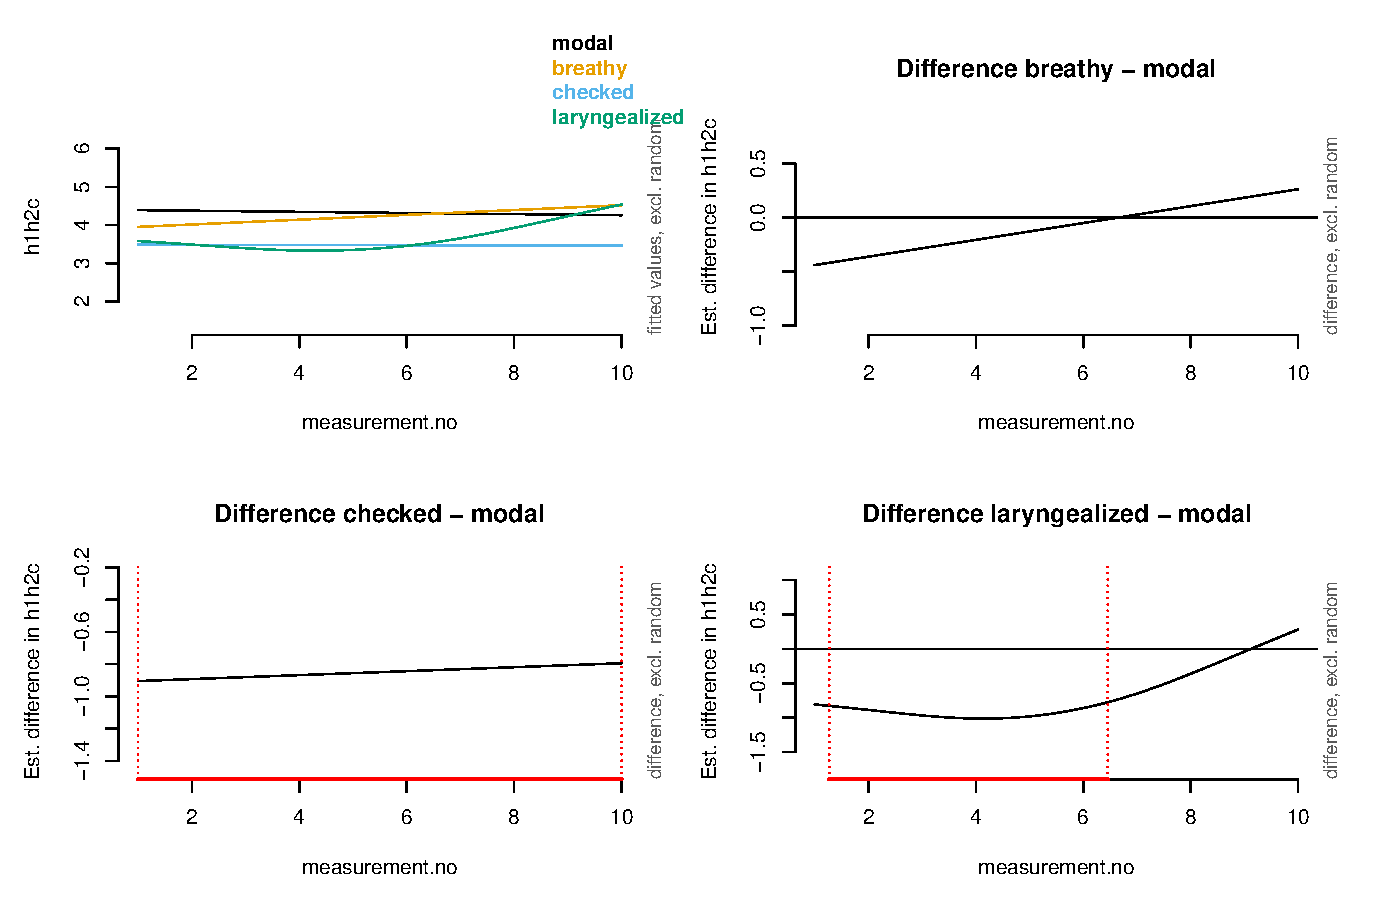
\includegraphics[width = \textwidth]{images/h1h2_gamm.eps}
  \caption{GAMM smooths and difference plots for H1*$-$H2* across the duration of the vowel.}
  \label{fig:GAMM_h1h2}
\end{figure}


The residual H1* GAMM showed a clearer distinction between the different voice qualities than H1*$-$H2*. This is especially clear in the smooth plot where the voice quality distinctions match with the predictions stated above. The difference plot in the top right shows that breathy and modal voice are only significantly different in the final two thirds of the vowel. The bottom left shows that checked and modal voice are significantly different across the entire duration of the vowel. Finally, the bottom right shows that rearticulated and modal voice are significantly different across the entire duration of the vowel.
\begin{figure}[!ht]
  \centering
  \includegraphics[width = \textwidth]{images/residh1_gamm.eps}
  \caption{GAMM smooths and difference plots for residual H1* across the duration of the vowel.}
  \label{fig:GAMM_residh1}
\end{figure}

In comparing the two GAMM analyses, we find that the residual H1* model provides a clearer distinction between the different voice qualities than the H1*$-$H2* model. This is further evidence that residual H1* is a more robust measure of voice quality than H1*$-$H2* in Santiago Laxopa Zapotec. Additionally, the GAMM analysis shows that there appear to be some amount of phasing in the data, which the linear models where unable to capture. This is especially clear in the residual H1* model where the difference plots show that breathy voice is only significantly different from modal in the final two thirds of the vowel. This suggests that breathy voice is aligned with the end of the vowel. This is similar to the predictions made by \citet{silvermanLaryngealComplexityOtomanguean1997,silvermanPhasingRecoverability1997} about the alignment of non-modal phonation in laryngeally complex languages. This will be further discussed in Chapters~\ref{ch:testing_lc} and \ref{ch:modeling_lc}.

\section{Conclusion} \label{sec:Conclusion}

In conclusion, we find that residual H1* is a more robust measure of voice quality than H1*$-$H2* in Santiago Laxopa Zapotec. This is supported by the results of the linear mixed-effects models, which show that residual H1* is better at distinguishing breathy, checked, and rearticulated vowels from modal vowels. This is further supported by the AIC comparison, which shows that the residual H1* model is a better fit for the data than the H1*$-$H2* model. These results lend credence to the claims of \citet{chaiH1H2AcousticMeasure2022} and support using residual H1* instead of H1*$-$H2* in voice quality research, especially in laryngeally complex languages.

However, the results neither suggest nor support the notion that residual H1* should be the sole measure used to determine phonation quality. Instead, we suggest that residual H1* should be included as one of the measures that researchers should consult during their acoustic studies. 
\chapter{The acoustic space of voice quality in Santiago Laxopa Zapotec} \label{ch:acousticlandscape}

%--------------------------------------------------------------------------
\section{Introduction} \label{sec:acousticlandscape:intro}
%--------------------------------------------------------------------------

This chapter studies the acoustic dimension of voice quality in Santiago Laxopa Zapotec (SLZ) using a Multidimensional Scaling (MDS) analysis of acoustic data. MDS is a statistical method that reduces the dimensionality of a dataset and visualizes the relationships between data points. This study uses MDS to visualize the acoustic space of voice quality in SLZ. This analysis provides information on the acoustic correlates of voice quality in SLZ and contributes to our understanding of the phonetic properties of this under-documented language.

This study is based on the work conducted by \citet{keatingCrosslanguageAcousticSpace2023} on the acoustic space of voice quality in 11 languages. However, this study focuses on a single language, SLZ, and provides a detailed analysis of the acoustic properties of voice quality in this language. The results of this study will contribute to our understanding of the phonetic properties of SLZ and how the acoustic properties of voice quality in this language compare with other languages.

%--------------------------------------------------------------------------
\section{Methods} \label{sec:acousticlandscape:methods}
%--------------------------------------------------------------------------
%--------------------------------------------------------------------------
\subsection{Participants} \label{sec:acousticlandscape:participants}
%--------------------------------------------------------------------------
This study uses data collected from 10 native speakers of SLZ during the summer of 2022. Participants were recruited from the community of Santiago Laxopa, Oaxaca, Mexico. All participants were native speakers of SLZ. The participants were between 18 and 60 years old and consisted of five males and five females.
%--------------------------------------------------------------------------
\subsection{Recordings} \label{sec:acousticlandscape:recordings} 
%--------------------------------------------------------------------------
Participants were asked to perform a word list elicitation task consisting of 72 words. These words were selected to elicit the entire range of types of voice quality in SLZ, including modal voice, the two kinds of creaky (i.e., checked and rearticulated), and breathy voice. The words were selected based on previous research conducted as part of the Zapotec Language Project at the University of California, Santa Cruz \citep{ZapotecLanguageProject}. 
Because participants were not literate in SLZ, the word list was prompted for them by asking them ``How do you say [word in Spanish]?" by myself and another researcher in Zapotec. Participants were asked to respond with the desired word in the carrier phrase \textit{Shnia' [WORD] chonhe lhas} ``I say [WORD] three times.'' which was repeated three times. These utterances were recorded in a quiet environment using a Zoom H4n digital recorder. The recordings were saved as 16-bit WAV files with a sampling rate of 44.1 kHz.

%--------------------------------------------------------------------------
\subsection{Acoustic measuring} \label{sec:acousticlandscape:analysis}
%--------------------------------------------------------------------------

The resulting audio files were then processed in Praat to isolate the vowel portion of each word. The onset of the vowel was set to the second glottal pulse after the onset, and the offset of the vowel was set to the last glottal pulse before the decrease in amplitude at the end of the vowel \citep{garellekAcousticDiscriminabilityComplex2020}. The vowel was then extracted and saved as a separate file for analysis.

These vowels were fed into VoiceSauce \citep{shueVoiceSauceProgramVoice2011} to generate the acoustic measures for the studies discussed in this dissertation. Because many acoustic measures are based on the fundamental frequency, this measure was calculated using the STRAIGHT algorithm from \citep{kawaharaInstantaneousfrequencybasedPitchExtraction1998} to estimate the fundamental frequency in millisecond (ms) intervals. Once the fundamental frequency is calculated, VoiceSauce then uses an optimization function to locate the harmonics of the spectrum, finding their amplitudes.

VoiceSauce then uses the Snack Sound toolkit \citep{sjolanderSnackSoundToolkit2004} to find the frequencies and bandwidths of the first four formants, also at millisecond intervals. The amplitudes of the harmonics closest to these formant frequencies are located and treated as the amplitudes of the formants. These formant frequencies and bandwidths are used to correct the harmonic amplitudes for the filtering effects of the vocal tract, using \citeauthor{iseliAgeSexVowel2007}'s \citeyear{iseliAgeSexVowel2007} extension of the method employed by \citet{hansonGlottalCharacteristicsFemale1997}. Each vowel was measured across ten equal time intervals, resulting in 22890 data points in total. These measures were then z-scored by speaker to reduce the variation between speakers and provide a way to compare the different measures directly on similar scales.

%--------------------------------------------------------------------------
\subsection{Data processing} \label{sec:acousticlandscape:data_processing}
%--------------------------------------------------------------------------
Data points with an absolute z-score value greater than three were considered outliers and excluded from the dissertation analyzes. The Mahalanobis distance was calculated in the F1-F2 panel within each vowel category. Each data point with a Mahalanobis distance greater than six was considered an outlier and excluded from the analysis.  

Energy was excluded if it had a zero value and then logarithmically transformed to normalize its right-skewed distribution. Afterward, the resulting log-transformed energy was z-scored and any data point with a z-score greater than three was excluded. This outlier removal resulted in 1918 data points being removed. 

All data points were then z-scored by speaker to reduce the variation between speakers and provide a way to compare the different measures directly on the same scale.

The residual H1 * was then calculated for the remaining data points following \citet{chaiH1H2AcousticMeasure2022}. First, a linear mixed effects model was generated with the z-scored H1* as the response variable and the z-scored energy as the fixed effect. The uncorrelated interaction of the z-scored energy by speaker was treated as random. The energy factor resulting from this linear mixed-effects model was extracted. Finally, the z-scored H1* had the product of the z-scored energy and the energy factor subtracted from it to produce the residual H1* measure. 

Once these steps were completed, the mean of each combination of phonation and speaker was taken for the fourth to seventh interval of the vowel. This is similar to what \citet{keatingCrosslanguageAcousticSpace2023} did by taking the middle of the vowel for their analysis. This choice minimizes the effect of the onset and offset of the vowel on the acoustic measures, which are more likely to be affected by the surrounding consonants and should give us the most accurate representation of the vowel quality. Because z-scores were used, this resulted in negative measures, which presents a problem for MDS analyses. To correct for this, I added the absolute value of the minimum z-score to each measure. This results in a dataset that still preserves the relative differences in the scores while providing a dataset that is all positive for the MDS analysis.

%--------------------------------------------------------------------------
\subsection{Statistical analysis} \label{sec:acousticlandscape:statistics}
%--------------------------------------------------------------------------

Multidimensional scaling analysis (MDS) is a type of dimensionality reduction to visualize the relationships between data points \citep{kruskalMultidimensionalScaling1978}. Using MDS is especially effective when many variables could contribute to the data. In the case of voice quality, this is especially warranted. 

As shown in \citet{kreimanUnifiedTheoryVoice2014,kreimanValidatingPsychoacousticModel2021,garellekAcousticDiscriminabilityComplex2020}, voice quality is psychoacoustically complex and a single measure is not enough to capture the full range of voice quality. Instead, multiple measures are required that function as cues for the different types of voice quality. For example, a vowel characterized as having a breathy voice has an elevated spectral-slope and a lower harmonics-to-noise ratio than a modal voice. A creaky voice has a lowered spectral-slope and a lowered harmonics-to-noise ratio. 

Because MDS analyses that contain many variables can result in rather unmeaningful results, I chose to focus on the speaker by phonation interaction. This allows us to see how speakers differ in their production of the different voice qualities. This choice to focus on speaker by phonation means that each speaker's production of each of the four phonation contrasts is represented as a single point in the MDS plot (e.g., one point for the first speaker's modal voice, one for their checked voice, one for their rearticulated voice, and one for their breathy voice). This is similar to what \citet{keatingCrosslanguageAcousticSpace2023} did in their study of the acoustic space of voice quality in 11 languages, except that they compared the language by voice quality interaction. Both of these interactions show us similar information. The analysis of speaker-by-voice quality shows us the acoustic space within a language, while the analysis using language-by-voice quality shows us the acoustic space between languages.

The MDS analysis was conducted using the \texttt{metaMDS} function in the \texttt{vegan} package \citep{oksanenVeganCommunityEcology2025} in the R programming language \citep{rcoreteamLanguageEnvironmentStatistical2024}. The Manhattan distance was used to estimate the differences between the speaker-by-phonation pairs. Because the distances are non-Euclidean, the MDS analysis was conducted using the nonmetric option.

This algorithm resulted in a solution that involves several different dimensions. The number of dimensions retained directly affects how well the original data is captured. Too many dimensions and the data are overfitted; too few, and the data are underfitted. To determine the number of dimensions to retain, I used a scree plot to plot the stress of each dimension. As shown in Figure~\ref{fig:stress_plot}, most of the data are captured in the first four dimensions. These four dimensions were retained for the analysis.

\begin{figure}[!ht]
    \centering
    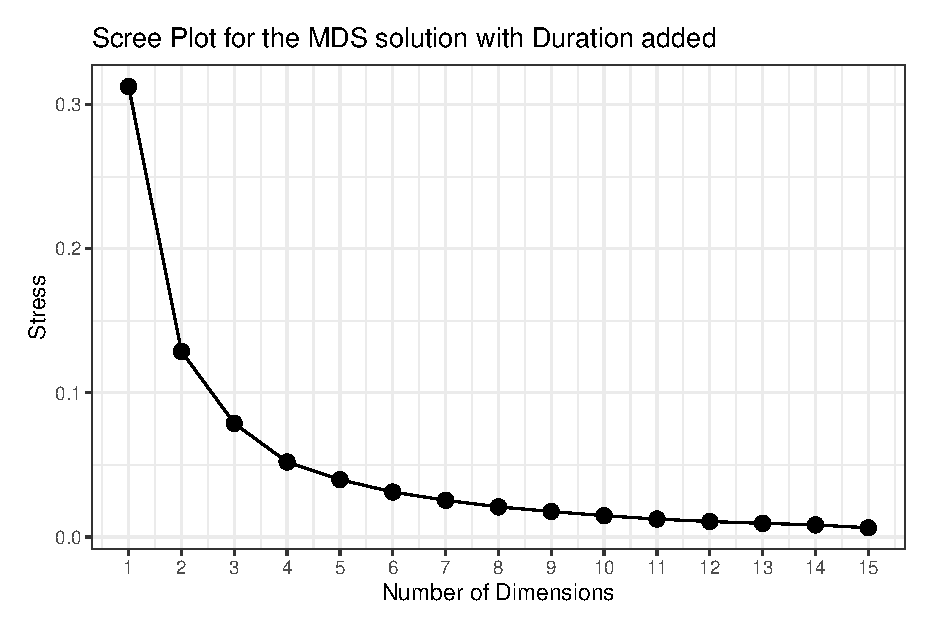
\includegraphics[width = 0.9\linewidth]{images/MDS/stress_plot_dur.eps}
    \caption{Scree plot showing the stress for each dimension for the MDS analysis.}
    \label{fig:stress_plot}
\end{figure}

% \begin{figure}[!h]
%     \centering
%     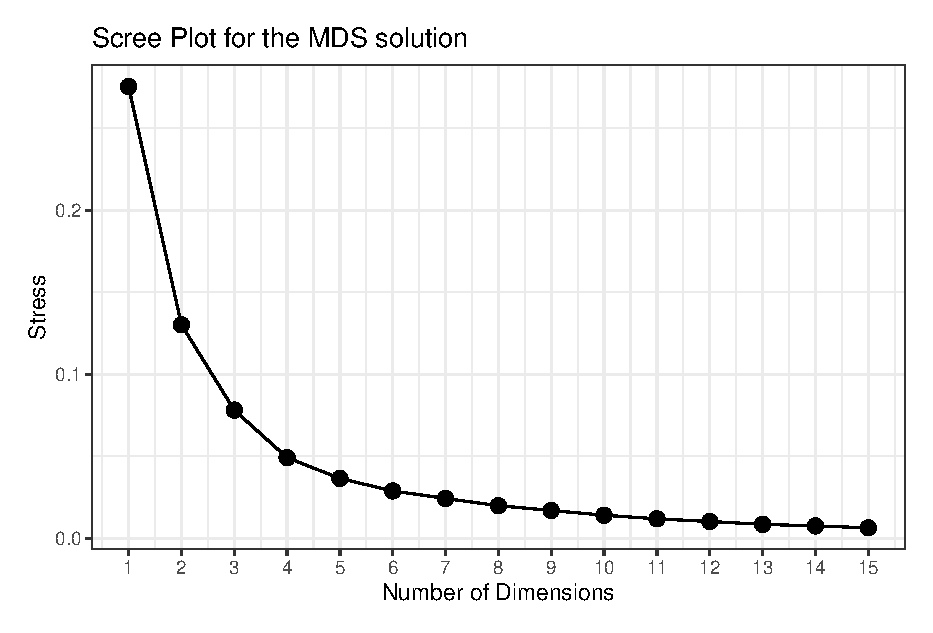
\includegraphics[width = 0.9\linewidth]{images/stress_plot_4:7.eps}
%     \caption{Scree plot showing the stress for each dimension for the MDS analysis.}
%     \label{fig:stress_plot}
% \end{figure}

%--------------------------------------------------------------------------
\section{Results} \label{sec:acousticlandscape:results}
%--------------------------------------------------------------------------
%--------------------------------------------------------------------------
\subsection{Acoustic space of voice quality} \label{sec:acousticlandscape:space}
%--------------------------------------------------------------------------

The results of the MDS analysis show that the acoustical space is represented primarily by a three-dimensional space.\footnote{A 3D plot showing the acoustic space can be found at \href{https://www.mlbrinkerhoff.me/files/3d_plot.html}{https://www.mlbrinkerhoff.me/files/3d_plot.html}.} In all subsequent plots, breathy voice is represented by orange, checked voice with blue, rearticulated voice with green, and modal voice with black. In each of the plots, the modal voice is generally more densely packed than the non-modal voice qualities. This is likely due to the fact that the modal voice represents approximately 60\% of the data, while the non-modal voice qualities represent approximately 40\% of the data. 
% The exact proportions of the data are given in Table~\ref{tab:voice_quality_proportions}.

% \begin{table}[ht]
%     \centering
%     \caption{Proportions of the different voice qualities in the dataset.} 
%     \label{tab:voice_quality_proportions}
%     \begin{tabular}{cccc}
%         \lsptoprule
%         Modal & Breathy & Checked & Rearticulated \\ 
%         \hline
%         0.62707838  &  0.14441805  &  0.09738717  &  0.13111639 \\
%         \lspbottomrule
%     \end{tabular}
% \end{table}

Figure~\ref{fig:nmds12} shows the first dimension plotted against the second dimension. In this plot, we observe that breathy voice is located in the top left of the plot, modal voice is located in the bottom center of the plot, and the two types of creaky voices are located to the right of the plot, with checked voice located at the extreme right of the plot, and rearticulated voice located closer to the center. From this plot, we see that the first dimension separates breathy, modal, and creaky voices. The second dimension separates the modal voice, bottom of the plot, from the non-modal voice qualities, top of the plot.

\begin{figure}[!ht]
    \centering
    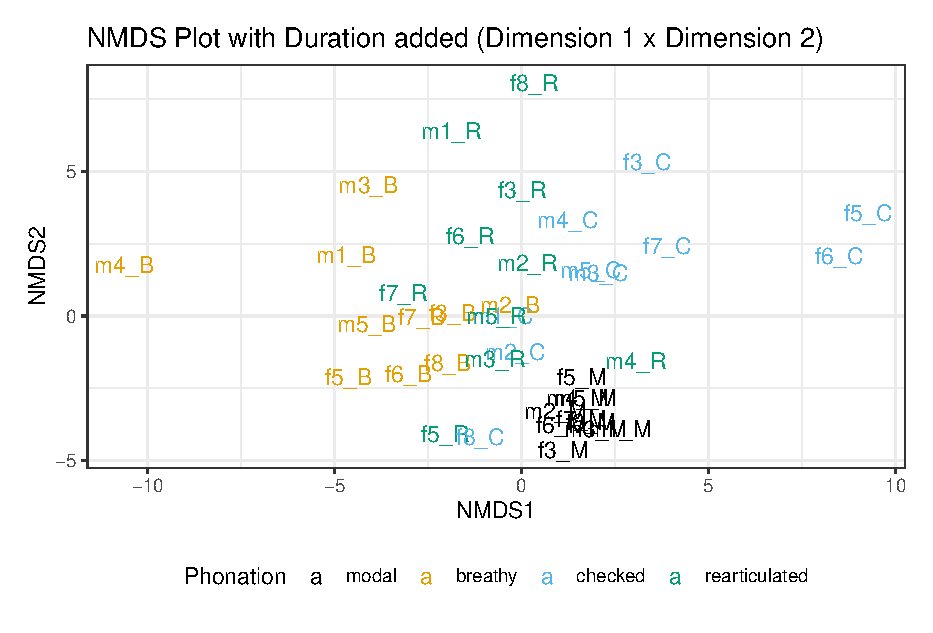
\includegraphics[width = 0.9\linewidth]{images/MDS/nmds12_dur.eps}
    \caption{Two-dimensional MDS solution showing the first and second dimensions.}
    \label{fig:nmds12}
\end{figure}

\begin{figure}[!ht]
    \centering
    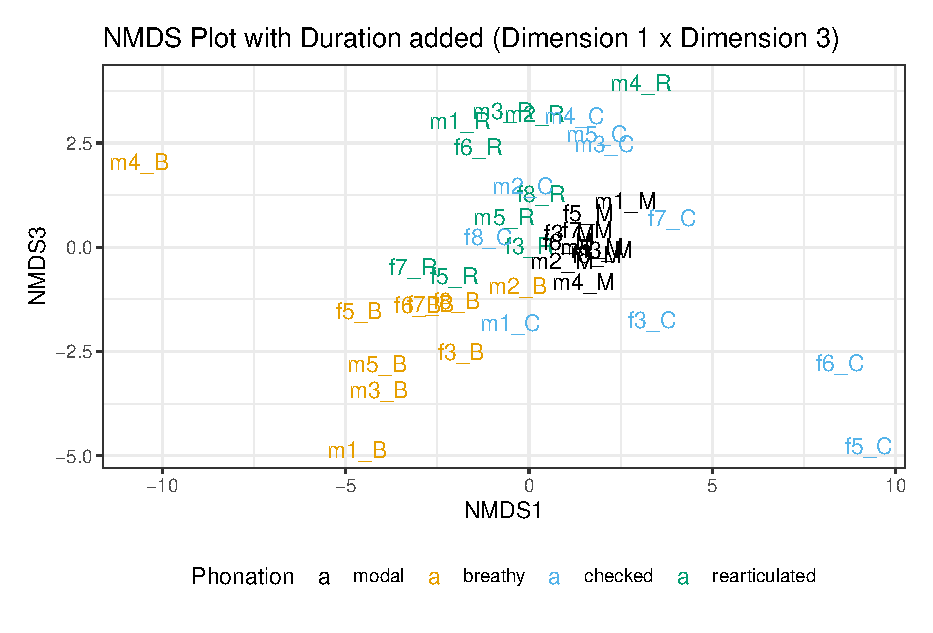
\includegraphics[width = 0.9\linewidth]{images/MDS/nmds13_dur.eps}
    \caption{Two-dimensional MDS solution showing the first and third dimensions.}
    \label{fig:nmds13}
\end{figure}

Figure~\ref{fig:nmds13} compares the first dimension with the third dimension. In this plot, we observe that the breathy voice is located in the bottom left of the plot, modal voice is located in the very center of the plot, and the two types of creaky voices are located in the top right of the plot. It should be noted that the distribution of the different voice qualities follows a line from bottom left to top right in the plot. This suggests that the first and third dimensions capture similar information about voice quality in SLZ.

% \begin{figure}[!h]
%     \centering
%     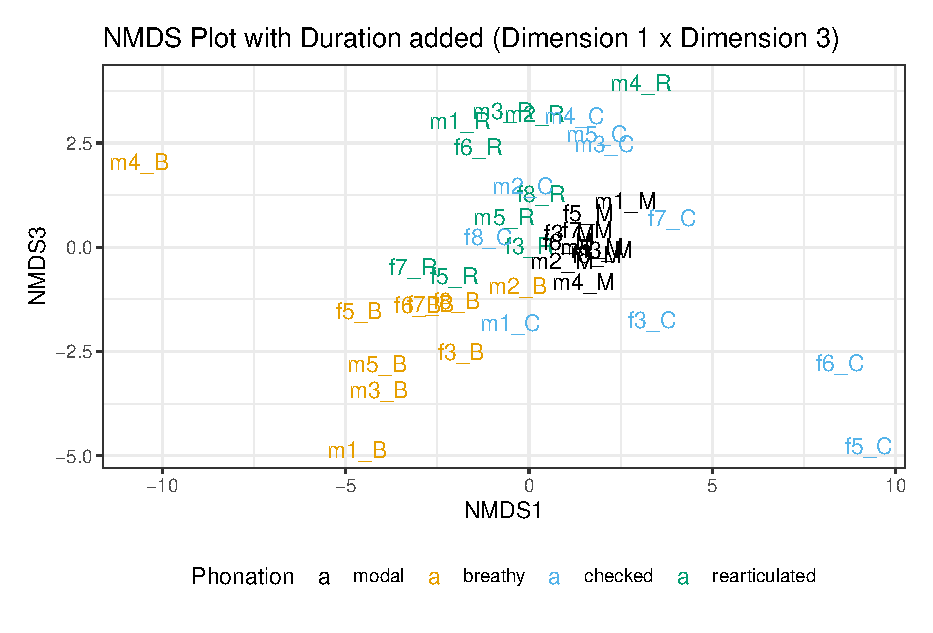
\includegraphics[width = 0.9\linewidth]{images/MDS/nmds13_dur.eps}
%     \caption{Two-dimensional MDS solution showing the first and third dimensions.}
%     \label{fig:nmds13}
% \end{figure}

Figure~\ref{fig:nmds14} shows the first dimension plotted against the fourth dimension. This plot is very similar to Figure~\ref{fig:nmds12}, with the only difference being that the fourth dimension moves the modal voice from the bottom-center of the plot to almost the exact center of the plot.

\begin{figure}[!ht]
    \centering
    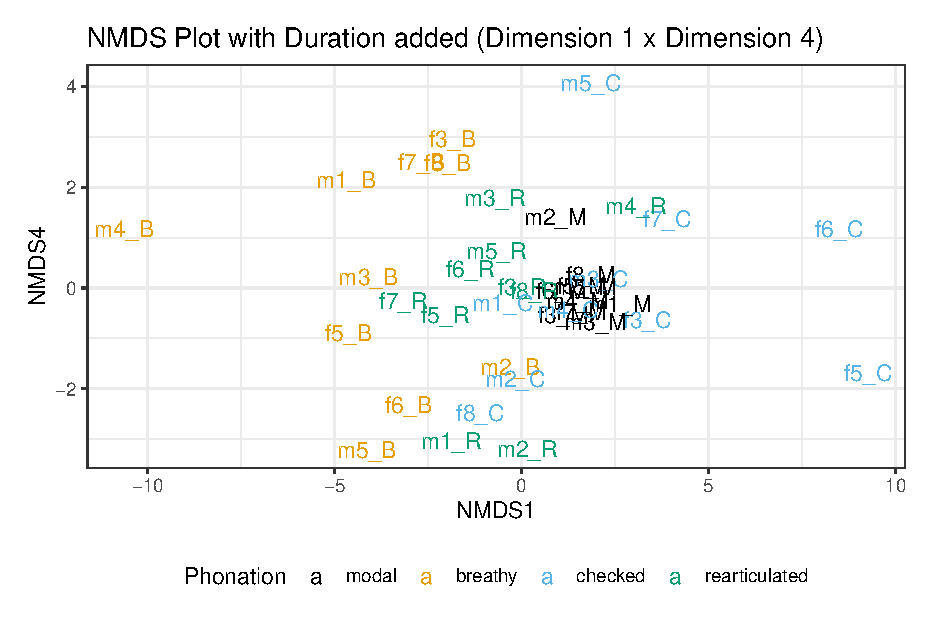
\includegraphics[width = 0.9\linewidth]{images/MDS/nmds14_dur.eps}
    \caption{Two-dimensional MDS solution showing the first and fourth dimensions.}
    \label{fig:nmds14}
\end{figure}

Figure~\ref{fig:nmds23} shows the second dimension plotted against the third dimension. This plot is essentially the same as Figure~\ref{fig:nmds13}, except that the coordinates are flipped.

\begin{figure}[!ht]
    \centering
    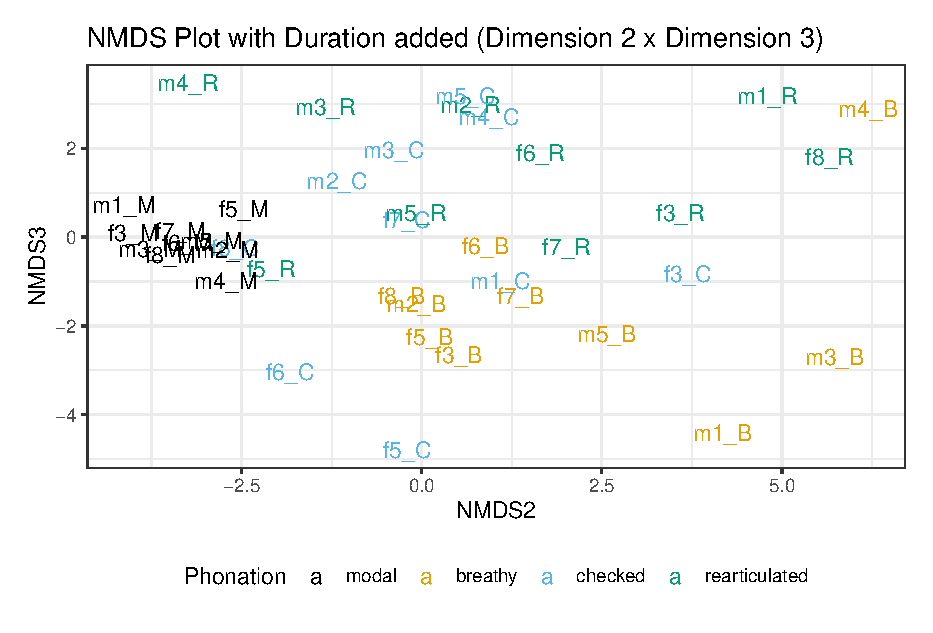
\includegraphics[width = 0.9\linewidth]{images/MDS/nmds23_dur.eps}
    \caption{Two-dimensional MDS solution showing the second and third dimensions.}
    \label{fig:nmds23}
\end{figure}

Figure~\ref{fig:nmds24} shows the second dimension plotted against the fourth dimension. This plot shows that the modal voice and the non-modal voice are separated into two different clusters, with modal voice located to the extreme left of the plot and the nonmodal voice qualities located to the right of the modal grouping. Again, as first seen in Figure~\ref{fig:nmds14}, the fourth dimension centralizes the modal voice, but no discernible pattern is observed for the other phonations.

\begin{figure}[!h]
    \centering
    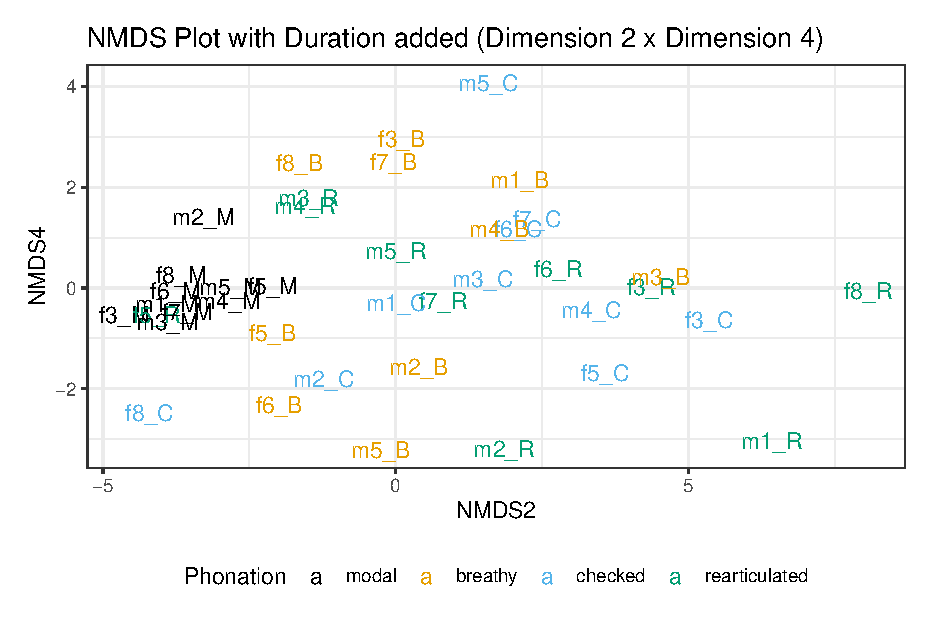
\includegraphics[width = \linewidth]{images/MDS/nmds24_dur.eps}
    \caption{Two-dimensional MDS solution showing the second and fourth dimensions.}
    \label{fig:nmds24}
\end{figure}

Figure~\ref{fig:nmds34} shows the third dimension plotted against the fourth dimension. This plot is very similar to Figure~\ref{fig:nmds14} with the exception that along the third dimension checked and rearticulated voice have swapped places. Checked voice is more centralized in the plot, whereas rearticulated voice is located more to the right of the plot. Again, we observe that the modal voice is located in the center of the plot.

\begin{figure}[!ht]
    \centering
    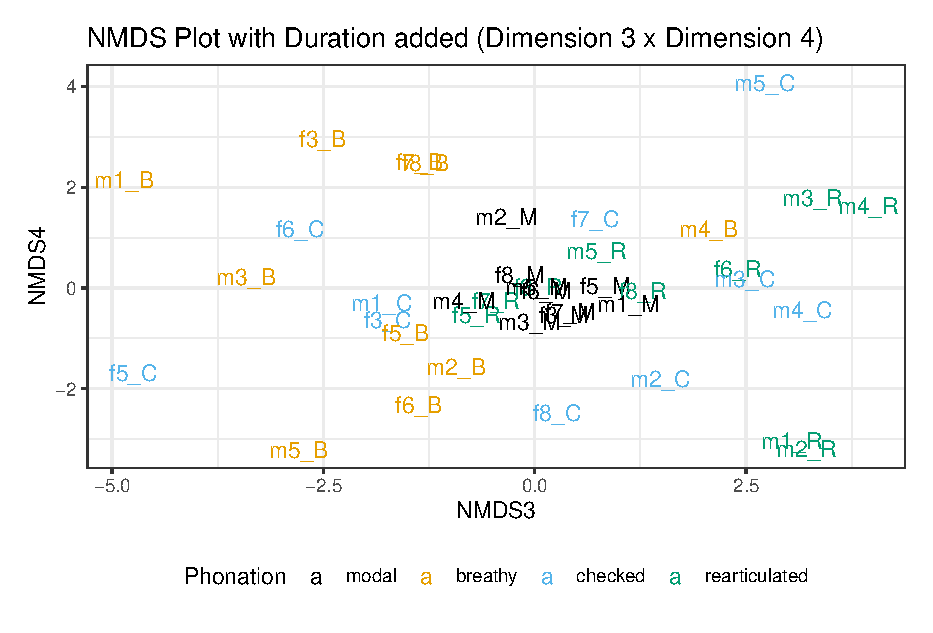
\includegraphics[width = 0.9\linewidth]{images/MDS/nmds34_dur.eps}
    \caption{Two-dimensional MDS solution showing the third and fourth dimensions.}
    \label{fig:nmds34}
\end{figure}

%--------------------------------------------------------------------------
\subsubsection{Interim summary for dimension plots} \label{sec:acousticlandscape:inter_sum}
%--------------------------------------------------------------------------

The plots of the MDS analysis show that the acoustic space of voice quality in SLZ is primarily represented by a three-dimensional space. The first dimension and third dimensions are very similar in that they capture a continuum from breathy, to modal, and finally creaky voice. This is similar to what \citet{keatingCrosslanguageAcousticSpace2023} found in their study for the second dimension. 

This continuum from breathy to modal to creaky is very similar to the open-quotient model of voice quality proposed by \citet{gordonPhonationTypesCrosslinguistic2001}, as illustrated in Figure~\ref{fig:phonation_types}. Because of this similarity to the open-quotient model, the first and third dimensions are likely capturing the open-quotient of the glottis. 

\begin{figure}[h!]
    \centering
    \begin{tikzpicture}
        % Draw the line with arrows at both ends
        \draw[<->, line width=0.5mm] (0,0) -- (10,0);
        
        % Labels underneath the line
        \node[below] at (0,0) {[h]};
        \node[below] at (2,0) {Breathy};
        \node[below] at (5,0) {Modal};
        \node[below] at (8,0) {Creaky};
        \node[below] at (10,0) {[ʔ]};
        
        % Labels above the line
        \node[above] at (0,0) {Open Glottis};
        \node[above] at (10,0) {Closed Glottis};
    \end{tikzpicture}
    \caption{A diagram showing the relationship between breathy, modal, and creaky phonation types from \citet{gordonPhonationTypesCrosslinguistic2001}.}
    \label{fig:phonation_types}
\end{figure}

From the plots involving the second dimension, we see that this dimension separates the modals from the non-modal ones. This is similar to what we observe with the various harmonics-to-noise ratios and the cepstral peak prominence (CPP) which are all measures of the amount of noise present in the signal across various bandwidths \citep{dekromCepstrumBasedTechniqueDetermining1993,hillenbrandAcousticCorrelatesBreathy1996,blankenshipTimingNonmodalPhonation2002,ferrerriesgoWhatMakesCepstral2020}. In addition to the amount of noise, it also captures the strength of the vocal fold vibration, similar to what \citet{garellekVoicingGlottalConsonants2021} found in their study of glottal consonants and nonmodals. In their study, they found that the modal voice had the highest strength of vocal fold vibration (measured by the Strength of Excitation), while the non-modal voice had a lower strength of vocal fold vibration. This suggests that the second dimension is to capture the amount of aperiodic noise in the signal, the strength of the vocal fold vibration, or both.

The fourth dimension is less clear about what it is potentially capturing. In all of the plots involving the fourth dimension, we see that modal voice is always located near the center of the plot, while the nonmodal voice qualities are located around this point depending on the patterns from the other dimensions. This suggests that the fourth dimension possibly captures something about modal voice. 

The rest of this chapter will focus on how the different acoustic measures contribute to the different dimensions of the MDS analysis. This will be followed by a general discussion of both the MDS analysis dimensions and the acoustic measures that are correlated with these dimensions. This discussion will focus on how the results of this study relate to previous work on voice quality and the implications of these results for our understanding of the acoustic space of voice quality. 

%--------------------------------------------------------------------------
\subsection{Acoustic correlates of voice quality} \label{sec:acousticlandscape:correlates}
%--------------------------------------------------------------------------

Looking at the visual representation of the dimensions is only part of the full story. In order to fully understand what is occurring, we need to determine how the acoustic measures contribute to each of the different dimensions. There are two ways to do this: (i) looking at the amount of weight each acoustic measure contributes to the different dimensions, and (ii) looking at how correlated the different acoustic measures are to the different dimensions \citep{kruskalMultidimensionalScaling1978,hastieElementsStatisticalLearning2009}. Both of these methods are useful in understanding the shape of the data. In the following discussion, I will take the second approach and look at the correlations between the different acoustic measures and the different dimensions. This is done to make the resulting discussion easier to follow.   

Table~\ref{tab:acoustic_correlates} shows the correlation score, computed by the \texttt{cor} function in R, for each acoustic measure and dimension. The four largest correlations in each dimension are in bold. The choice to bold the four largest correlations was arbitrary and was done to make it easier to discuss. Although only the four largest correlations are bolded, there are several correlations that share similar correlation values. These cases will be discussed as needed.

\begin{table}[!ht]
    \centering
    \caption{Correlations for each acoustic measure to the four dimensions (NMDS1, NMDS2, NMDS3, NMDS4). The four largest correlations in each dimension are bolded.} 
    \label{tab:acoustic_correlates}
    \begin{tabular}{lrrrr}
        \lsptoprule
        Acoustic Measure & NMDS1 & NMDS2 & NMDS3 & NMDS4 \\ 
        \hline
        H1*$-$H2* & -0.221 & -0.339 & 0.031 & 0.314 \\ 
        H2*$-$H4 & -0.437 & 0.239 & \textbf{-0.689} & \textbf{-0.364} \\ 
        H1*$-$A1* & \textbf{-0.828} & 0.048 & \textbf{-0.459} & 0.044 \\ 
        H1*$-$A2* & \textbf{-0.855} & -0.067 & -0.343 & 0.114 \\ 
        H1*$-$A3* & \textbf{-0.809} & -0.218 & -0.297 & 0.126 \\ 
        H4*$-$H2k* & -0.452 & -0.598 & 0.294 & \textbf{0.366} \\ 
        H2k*$-$H5k* & 0.152 & 0.023 & 0.101 & 0.057 \\ 
        residual H1* & -0.290 & -0.443 & \textbf{-0.722} & 0.084 \\ 
        H2* & -0.157 & -0.555 & \textbf{-0.679} & 0.114 \\ 
        H4* & 0.295 & \textbf{-0.778} & 0.078 & \textbf{0.479} \\ 
        A1* & 0.756 & -0.549 & 0.092 & 0.124 \\ 
        A2* & \textbf{0.779} & -0.476 & -0.103 & 0.086 \\ 
        A3* & 0.735 & -0.416 & -0.211 & 0.093 \\ 
        CPP & -0.590 & -0.606 & 0.209 & -0.179 \\ 
        HNR < 500 Hz & -0.513 & \textbf{-0.792} & 0.152 & -0.202 \\ 
        HNR < 1500 Hz & -0.275 & \textbf{-0.799} & 0.323 & -0.290 \\ 
        HNR < 2500 Hz & -0.327 & -0.714 & 0.391 & -0.348 \\ 
        HNR < 3500 Hz & -0.446 & -0.644 & 0.393 & -0.356 \\ 
        Strength of Excitation & -0.013 & -0.741 & -0.238 & 0.145 \\ 
        SHR & 0.144 & -0.176 & 0.122 & \textbf{-0.597} \\ 
        Energy & -0.080 & \textbf{-0.793} & -0.015 & 0.341 \\ 
        Duration & -0.622 & 0.539 & 0.257 & 0.030 \\ 
        \lspbottomrule
    \end{tabular}
\end{table}

%--------------------------------------------------------------------------
\subsubsection{Dimension 1} \label{sec:acousticlandscape:dim1}
%--------------------------------------------------------------------------
From Table~\ref{tab:acoustic_correlates}, we observe that the first dimension is negatively correlated with the acoustic slope measures of H1*$-$A1*, H1*$-$A2*, and H1*$-$A3* ($r^{2} \approx -0.825$ for all three of these measures). These measures are all types of spectral slope measures which attempt to normalize the amplitude of the formant corrected H1 against the amplitudes of the formant correct harmonic closest to the first three formants. It has been noted that these measures are correlated with the open-quotient of the glottis (see \cite{garellekPhoneticsVoice2019,garellekTheoreticalAchievementsPhonetics2022} for an overview of these measures). Because these measures all capture the same information and they are all highly correlated with the first dimension, we can conclude that the first dimension is primarily concerned with the spectral slope of the signal (i.e., the open-quotient of the glottis). 

The first dimension is also positively correlated with the amplitude of the first three formants (that is, A1*, A2*, and A3*). These acoustic measures also share correlations of a similar value ($r^{2} \approx 0.75$). It is also worth noting that these amplitude measures are all used in the normalization of the spectral slope measures (i.e., H1*$-$A1*, H1*$-$A2*, and H1*$-$A3*). I believe that this fact suggests that the first dimension is primarily concerned with the spectral slope of the signal, but is also factoring in the amplitude of the formants.

%--------------------------------------------------------------------------
\subsubsection{Dimension 2} \label{sec:acousticlandscape:dim2}
%--------------------------------------------------------------------------
The second dimension is strongly correlated with the harmonics-to-noise ratio (HNR) measures. The HNR measures HNR < 500 Hz, HNR < 1500 Hz, and HNR < 2500 Hz are all negatively correlated with the second dimension ($r^{2} \approx -0.79$). These measures are all measures of the amount of noise in the signal and are used to indicate the amount of periodicity in the signal (e.g., whether something is modal or non-modal). This suggests that the second dimension is concerned with the amount of noise in the signal.

Furthermore, there are strong negative correlations with energy, which is the root mean squared energy of the acoustic signal, and the Strength of Excitation (SoE), which is defined as ``the instant of significant excitation of the vocal-tract system during production of speech'' and represents ``the relative amplitude of impulse-like excitation'' \citep[1934]{mittalStudyEffectsVocal2014}. In other words, the SoE correlates with how strongly the vocal folds vibrate during the signal with modal voice showing the strongest amount of voicing and nonmodal phonation the least. This suggests that the second dimension is also concerned with strength of the vocal-fold vibration.

The last measure that shows a strong correlation with the second dimension is the amplitude of the fourth harmonic (H4*). This measure is negatively correlated with the second dimension ($r^{2} \approx -0.78$). This measure is typically used to help normalize the amplitude of the first formant and is used in the calculation of the spectral slope measures (e.g., H2*$-$H4*).

Together, given the correlations of the HNR measures, energy, and SoE, we can conclude that the second dimension is primarily concerned with the periodicity of the signal (i.e., the amount of noise in the signal) and the strength of the vocal fold vibration.

%--------------------------------------------------------------------------
\subsubsection{Dimension 3} \label{sec:acousticlandscape:dim3}
%--------------------------------------------------------------------------
The third dimension is negatively correlated with the two spectral slope measures of residual H1* and H2*$-$H4* ($r^{2} \approx -0.7$). Residual H1* is a measure that has been shown to be robust in capturing the strength of the first harmonic \citep{chaiH1H2AcousticMeasure2022,brinkerhoffUsingResidualH12025}, which was the original goal of using higher harmonics to normalize H1 \citep{fischer-jorgensenPhoneticAnalysisBreathy1968}. H2*$-$H4* has also been shown to be another spectral slope measure that can capture the differences in amplitude between different phonation types \citep{garellekPhoneticsVoice2019,garellekModelingVoiceSource2016,kreimanUnifiedTheoryVoice2014,kreimanValidatingPsychoacousticModel2021}. This suggests that the third dimension is primarily concerned with the spectral slope of the signal, similar to what we observed in the first dimension.

In addition to these measures, the amplitude of the second harmonic (H2*) was also found to be negatively correlated with the third dimension ($r^{2} \approx -0.69$). This measure is typically used to help normalize the amplitude of the first harmonic and is used in the calculation of the spectral slope measures (e.g., H1*$-$H2*, H2*$-$H4*, etc.). Due to its use in spectral slope measures and that H2*$-$H4* is also negatively correlated with the third dimension, we can conclude that H2 * also contributes to the spectral slope of the signal. This further supports the idea that the third dimension is primarily concerned with the spectral slope of the signal. 

The last acoustic measure also correlated with the third dimension is the spectral slope measure of H1*$-$A1* ($r^{2} \approx -0.46$). Even though the correlation is not as strong as the other acoustic measures, it still shows that the third dimension corresponds to the spectral slope of the signal (i.e., the open-quotient of the glottis).

%--------------------------------------------------------------------------
\subsubsection{Dimension 4} \label{sec:acousticlandscape:dim4}
%--------------------------------------------------------------------------

In the fourth dimension, we observe that the correlations are less clear than in the previous three dimensions. The strongest correlations in this dimension with the Subharmonic-to-Harmonic ratio (SHR; $r^{2} \approx -0.60$) describe the relative strength of any subharmonics (interharmonics) in the signal \citep{sunPitchDeterminationVoice2002}. The subharmonics in the signal correspond to alternating periods in the time domain (that is, period doubling), which typically occurs in creaky voice and with broader laryngeal constrictions (see \cite{herbstPerformanceEvaluationSubharmonictoHarmonic2021} for concerns about this acoustic measure). 

The positive correlation with H4* ($r^{2} \approx 0.48$) suggests that the fourth dimension may also capture some information about the amplitude of the higher harmonics. This is also true with the positive correlation with H4*$-$H2k* ($r^{2} \approx 0.37$) and H2*$-$H4* ($r^{2} \approx 0.36$), which are both measures that capture the spectral slope of the signal. This suggests that the fourth dimension may capture information about the amplitude of the harmonics in the signal. 

%--------------------------------------------------------------------------
\subsubsection{Interim summary for acoustic correlates} \label{sec:acousticlandscape:interim_correlates}
%--------------------------------------------------------------------------

Based on the correlations observed in Table~\ref{tab:acoustic_correlates}, we can summarize the acoustic correlates of each dimension as follows: Dimension 1 captures the spectral slope of the signal, primarily through the spectral slope measures H1*$-$A1*, H1*$-$A2*, and H1*$-$A3*. This dimension appears to be related to the open-quotient of the glottis. Dimension 2 captures the amount of noise in the signal and the strength of vocal fold vibration, primarily through the HNR measures (HNR < 500 Hz, HNR < 1500 Hz, and HNR < 2500 Hz), Energy, and Strength of Excitation. This dimension separates modal from nonmodal voice quality, which is what periodicity is concerned with. Dimension 3 captures the spectral slope of the signal as well, just as Dimension 1 does, primarily through residual H1*, H2*$-$H4*, and H2*. This dimension also appears to be related to the open-quotient of the glottis. Finally, Dimension 4 captures the periodicity in the signal through SHR and also appears to capture some information about the spectral slope, as evidenced by the amplitude of the higher harmonics through H4* and H4*$-$H2k*. However, it is not entirely clear whether this dimension is primarily concerned with the spectral slope of the signal or the periodicity in the signal.

%--------------------------------------------------------------------------
\section{Discussion} \label{sec:acousticlandscape:discussion}
%--------------------------------------------------------------------------

The results of this study show that the voice quality in SLZ occupies an acoustic space, but also shows that this space is similar to what \citet{keatingCrosslanguageAcousticSpace2023} found in their study of phonation in 11 languages. However, the results of this study differ from \citet{keatingCrosslanguageAcousticSpace2023}. Instead of a two-dimensional space like in \citet{keatingCrosslanguageAcousticSpace2023}, SLZ's voice quality occupies a three-dimensional space. Despite these differences, the behavior of the dimensions is similar to that in \citet{keatingCrosslanguageAcousticSpace2023}. 

In the analysis presented in this chapter, we see that the first and third dimensions are primarily concerned with a spectral slope continuum from positive spectral slope to negative spectral slope which correlates to breathy voice to modal voice and finally to creaky voice. As extensive research has shown, the spectral slope of the signal is closely related to the open-quotient of the glottis, or in other words, how open or closed the glottis is during phonation (see \citet{garellekTheoreticalAchievementsPhonetics2022} for an overview of this history). This continuum was also found to exist in the second dimension of \citeauthor{keatingCrosslanguageAcousticSpace2023}'s \citeyear{keatingCrosslanguageAcousticSpace2023} MDS analysis. Based on \citet{keatingCrosslanguageAcousticSpace2023} and the analysis presented in this chapter, at least one of the dimensions of any acoustic space related to voice quality must correspond to the spectral slope of the signal. 

As mentioned in Section~\ref{sec:acousticlandscape:inter_sum}, the first and third dimensions of this chapter's analysis and \citeauthor{keatingCrosslanguageAcousticSpace2023}'s second dimension, bear a striking resemblance to the voice quality model proposed by \citet{gordonPhonationTypesCrosslinguistic2001}. In \citeauthor{gordonPhonationTypesCrosslinguistic2001}'s model, voice quality is described as being a single continuum based on how open or closed the glottis is during speech. The more open the glottis, the more breathy the phonation will be. The more closed the glottis, the more creaky the phonation will be. This model also claims that laryngeal consonants [h] and [ʔ] also exist along this continuum and represent the extreme ends of this continuum.  This model can be visually represented as a line with [h] on one end and [ʔ] on the other end. The various voice qualities exist between these two extremes, as represented in Figure~\ref{fig:phonation_types_1}.

\begin{figure}[h!]
    \centering
    \begin{tikzpicture}
        % Draw the line with arrows at both ends
        \draw[<->, line width=0.5mm] (0,0) -- (10,0);
        
        % Labels underneath the line
        \node[below] at (0,0) {[h]};
        \node[below] at (2,0) {Breathy};
        \node[below] at (5,0) {Modal};
        \node[below] at (8,0) {Creaky};
        \node[below] at (10,0) {[ʔ]};
        
        % Labels above the line
        \node[above] at (0,0) {Open Glottis};
        \node[above] at (10,0) {Closed Glottis};
    \end{tikzpicture}
    \caption{A diagram showing the relationship between breathy, modal, and creaky phonation types. Based on \citet{gordonPhonationTypesCrosslinguistic2001}.}
    \label{fig:phonation_types_1}
\end{figure}

As mentioned above, the measures that correlate the most with the first and third dimensions are several spectral slope measures (i.e., H1*$-$A1*, H1*$-$A2*, H1*$-$A3*, residual H1*, and H2*-H4*). These measure correlations provide further support that the first and third dimensions of the MDS analysis are concerned with the spectral slope of the signal, which in turn is closely correlated with the state of the glottis during phonation \citep{holmbergComparisonsAerodynamicElectroglottographic1995,kreimanMeasuresGlottalSource2007,garellekModelingVoiceSource2016,garellekPhoneticsVoice2019,chaiH1H2AcousticMeasure2022}.

The second dimension of this chapter's analysis is concerned with dividing the acoustic space into modal and nonmodal voice qualities. This split between modal and nonmodal is similar to the split that exists for periodicity and strength of voicing. The more modal the voice quality is, the greater the amount of periodicity or voicing that we observe in the signal. I propose that this dimension is concerned with how harmonic the signal is, or in other words, how much noise is present in the acoustic signal. This is similar to what \citet{keatingCrosslanguageAcousticSpace2023} found in their study, where the first dimension of their analysis was primarily concerned with making the same split in the acoustic space. Based on these results, I propose that another dimension in the acoustic space of voice quality must correspond to the amount of noise in the signal. This proposal is further supported by the fact that the second dimension of this chapter's analysis is primarily correlated with the harmonics-to-noise ratios, energy, and SoE measures, which are all measures of the amount of noise or the amount of energy present in the acoustic signal. 

The last dimension of the MDS analysis is less clear in what it is capturing. The correlation with the subharmonics-to-harmonic ratio (SHR) suggests that this dimension might be capturing whether or not their is period doubling which is a common feature in creaky voice. However, there is no easily describable pattern that emerges with this measure. 

The results of this study show that the voice quality acoustic space in SLZ is primarily represented by a three-dimensional space. However, it can primarly be broken down into two aspects that the acoustic space is attempting to capture: (i) the spectral slope of the signal and (ii) the amount of noise in the signal. This can be represented as a primarily two-dimensional space with higher dimensions adding additional information related to these two primary concerns. This can be visualized as a two-dimensional space with the first dimension representing the spectral slope of the signal and the second dimension representing the amount of noise in the signal, as shown in Figure~\ref{fig:acoustic_space}.

\begin{figure}[h!]
    \centering
    \begin{tikzpicture}
        % Draw the horizontal line with arrows
        \draw[<->, line width=1.5mm] (-4,0) -- (4,0);
        % Draw the vertical line with arrows
        \draw[<->, line width=1.5mm] (0,-4) -- (0,4);
        
        % Labels for the horizontal line
        \node[below,yshift=1cm] at (-4,0) {Lower Spectral Slope};
        \node[below,yshift=1cm] at (4,0) {Higher Spectral Slope};
        
        % Labels for the vertical line
        \node[left, xshift = -1.5mm] at (0,-3) {Less Harmonic};
        \node[left, xshift = -1.5mm] at (0,3) {More Harmonic};
    \end{tikzpicture}
    \caption{A two-dimensional representation of the acoustic space of voice quality in SLZ. The horizontal axis represents the spectral slope of the signal, while the vertical axis represents the amount of noise or energy in the signal.}
    \label{fig:acoustic_space}
\end{figure}

%--------------------------------------------------------------------------
\section{Conclusion} \label{sec:acousticlandscape:conclusion}
%--------------------------------------------------------------------------

Although the discussion has predominately been about the correlations of the measures that contribute to the different dimensions, it is important to note that the measures are not independent of each other. Instead, all of the measures contribute to the acoustic space of voice quality in SLZ to some extent or another. Just because a measure has a low correlation does not mean that it does not contribute to the acoustic space. Rather than thinking of the measures as independent of each other, it is better to think of them as a group of measures that work together to create the acoustic space of voice quality in SLZ. This is especially true given the fact that the MDS analysis is a reduction of the data to a few dimensions. This analysis offers a snapshot of the voice quality acoustic space in SLZ, but is not the full picture. 

Furthermore, as will be discussed in Chapter~\ref{ch:revealing_trees}, another way in which we can determine which measures are the most important is by performing a classification and regression tree analysis \citep{breimanClassificationRegressionTrees1986,breimanBaggingPredictors1996,breimanRandomForests2001}.
\chapter{Trees reveal the importance of measures in SLZ} \label{ch:revealing_trees}

%--------------------------
\section{Introduction} \label{sec:bagging_intro}
%--------------------------

The MDS analysis presented in Chapter~\ref{ch:acousticlandscape} provides us an understanding of the acoustic shape that voice quality takes in SLZ. This shape is defined by different dimensions that correspond to the glottal configuration needed to produce each voice quality and the amount of noise in the signal. The MDS analysis also provides us with a way to visualize how the different voice qualities occupy an acoustic space. Finally, the chapter discussed how different acoustic measures are correlated with the different dimensions of the acoustic space. This provides us with a potential avenue to explore which measures contribute to our understanding of the different voice qualities in SLZ.
However, the analysis does not tell us which measures are the most important in making the splits between the different voice qualities. This is where decision trees are helpful as they provide a way to cut through the noise and reveal which measures play the most important role in dividing that acoustic space. 

In this chapter, I present an anlysis using a flavor of decision trees called Random Forests \citep{breimanClassificationRegressionTrees1986,breimanRandomForests2001}. Random Forests are a type of ensemble learning method that combines multiple decision trees that are built on the same data. This allows us to take advantage of the strengths of decisions trees while minimizing the weaknesses that are present in classical decision trees (see \cite{hastieElementsStatisticalLearning2009,boehmkeHandsOnMachineLearning2019,jamesIntroductionStatisticalLearning2021} for a discussion of the strengths and weaknesses of the different types of decision trees).

I show in this chapter that only a small number of acoustic measures are needed to classify the different voice qualities and make the splits in the acoustic space. 

%--------------------------
\section{What are Decision Trees} \label{sec:what_are_dt}
%--------------------------

Decision trees are a statistical tool that helps to reveal which predictors divide the space under investigation. Essentially, this is done by stratifying or segmenting the predictor space into some number of simpler regions. The rules that divide the space into these regions are based on some aspect of the predictors (see \cite{hastieElementsStatisticalLearning2009,jamesIntroductionStatisticalLearning2021} for explanations on the statistics and how to perform these analyses in R). 

These trees can be used for both regression and classification. In the case of regressions, it splits the predictor space into regions and calculates how the item under discussion behaves in each region. This process of splitting into regions and calculating how something responds in that region continues until some stopping rule is applied, which is usually defined to some number of terminal nodes. This resulting tree is rather large and is then pruned based on the cost-complexity pruning to a subset of itself. This subsetted tree is the tree that has minimized its cost-complexity criterion of all potential subsets. Meaning that it balances the trade-off between the complexity of the tree and its fit to the data. 

In the case of classification, the algorithms that result in a tree are very similar to those used for regression trees. The main difference in algorithm comes from what is used to split the nodes and how the tree is pruned. Instead of predicting a continuous outcome like with regression trees, classification trees predict a categorical outcome. The predictor space is divided into regions, and within each region, the majority class is assigned as the predicted class for that region. This process continues until a stopping rule is applied, similar to regression trees. The resulting tree can also be pruned to avoid overfitting, using a cost-complexity criterion.

Decision trees are easy to interpret and visualize, making them an ideal choice for understanding the structure of data and how the different predictors interact with data \citep{hastieElementsStatisticalLearning2009,jamesIntroductionStatisticalLearning2021}.

%-----------------------------
\section{Decision trees in linguistics}\label{sec:dt_linguistics}
%-----------------------------

The use of decision trees in linguistics is not new. One of the first uses was done by \citet{tagliamonteModelsForestsTrees2012}, where they illustrated the use of decision trees in investigating which sociolinguistic factors were the most important in the use of \textit{was} versus \textit{were} in York English. 

Recently, decision trees were used to show which acoustic measures were the important in making the split in the acoustic space for voice quality \citep{keatingCrosslanguageAcousticSpace2023}. \citeauthor{keatingCrosslanguageAcousticSpace2023} performed a simple decision tree analysis to supplement their MDS analysis of voice quality in 11 languages. The results of this analysis are shown in Figure~\ref{fig:keating_tree}. Decision trees like the one in Figure~\ref{fig:keating_tree}, show the binary splits that are made in the space and what predictor, and the value of that predictor, makes that split. In the case of \citeauthor{keatingCrosslanguageAcousticSpace2023}'s (\citeyear{keatingCrosslanguageAcousticSpace2023}) tree, the first split is made on the harmonics-to-noise ratio over the frequency range from 0 Hz to 500 Hz for the middle third of each vowel. This split is made at the z-score of 0.48. If the value of the predictor is greater or equal to 0.48, the dominate voice quality of that region is modal. If HNR < 500 Hz value is less than 0.48, the region needs to be further split. 

\begin{figure}[!ht]
    \centering
    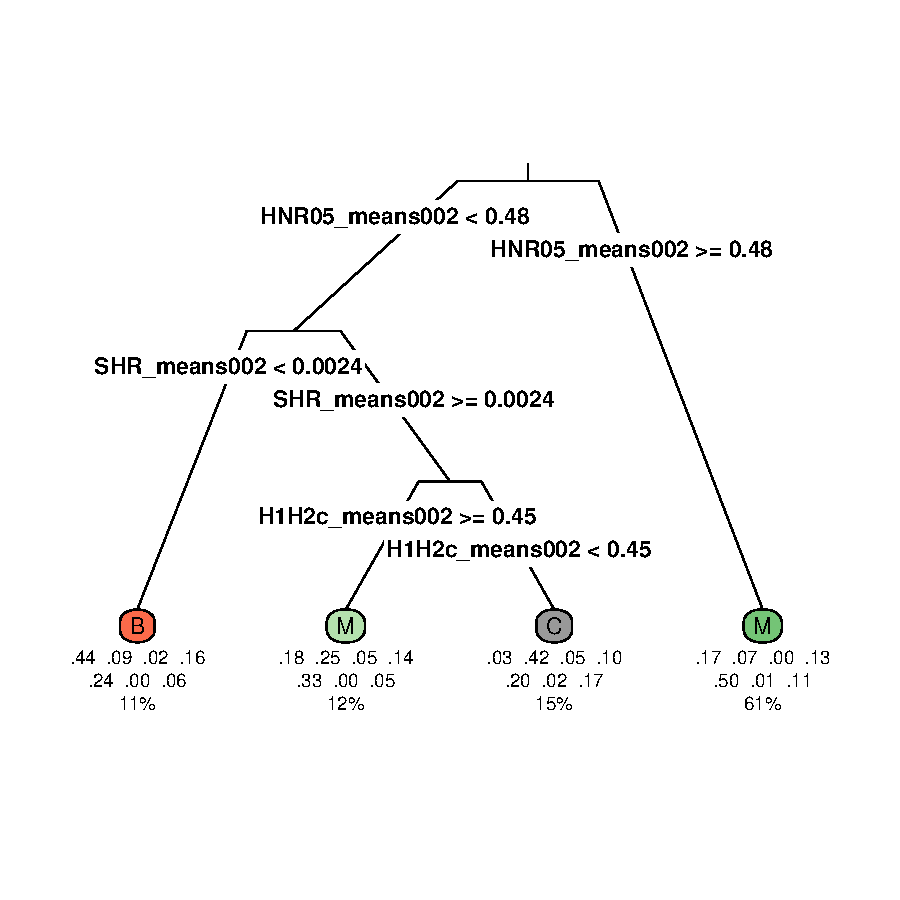
\includegraphics[width = 0.9\linewidth]{images/keating_tree.pdf}
    \caption{Classification tree of phonation categories from \citet{keatingCrosslanguageAcousticSpace2023}. Abbreviations used in this figure are: {HNR05_means002}: harmonics-to-noise ratio over the frequency range from 0 Hz to 500 Hz for the middle third of each vowel; {SHR_means002}: subharmonic-to-harmonic ratio for the middle third of each vowel; {H1H2c_means002}: H1* − H2* for the middle third of each vowel; B: breathy, M: modal, and C: creaky phonation categories.}
    \label{fig:keating_tree}
\end{figure}

The next split in the region is made on the subharmonic-to-harmonic ratio for the middle third of each vowel. If the value of this predictor is less than 0.0024, the voice quality is classified as breathy. If the value is greater than or equal to 0.0024, the region needs to be split further.

The final split in the region is made on the H1*$-$H2* for the middle third of each vowel. If the value of this predictor is less than 0.45, the voice quality is classified as creaky. If the value is greater than or equal to 0.45, the voice quality is classified as modal. This tree shows that using only three acoustic measure, one can classify the voice quality of the data. This is a powerful tool for understanding the importance of the different acoustic measures in the acoustic space. 

%--------------------------
\section{Growing a forest of decision trees} \label{sec:growing_forest}
%--------------------------

Simple decision trees, however, suffer from two main disadvantages. The first is that decision trees can suffer from high variance. In other words, the tree can be very sensitive to small changes in the data that it was trained on. The second disadvantage is that decision trees do not have the same predictive accuracy as other regression or classification models (see \cite{hastieElementsStatisticalLearning2009} for discussion).

%---------------------------
\subsection{Bagging trees} \label{sec:bagging_bagging}
%---------------------------
One way to overcome these disadvantages, is to make use of a technique called bootstrap aggregating, or bagging \citep{breimanBaggingPredictors1996}. This means that instead of growing a single tree with all of the predictors (i.e., variables in your data) in the data like in simple decision trees, we grow many trees on random samples of the data until we reach a given number of trees using the full set of predictors. Once these trees are grown, we then average across the trees to get a more stable prediction of how the regions are split and what predictors are most important in making those splits. This averaging across the trees help to explain the variance in the data and improve the predictive accuracy of the model. However, this comes at the cost of interpretability. 

In decision trees, we usually represent the splits in the data as a tree. When we using bagging, because of the large numbers of trees that are grown, it is impossible to represent the results in this way. Instead of using a tree, we use variable importance measures to understand which predictors are most important in making the splits in the data. There are two measures that are commonly used to understand variable importance in bagging trees: the residual sum of squares (RSS) for regression trees and the Gini index, which is a measure of \textit{purity}, for classification. In regression trees, the amount that the RSS is decreased due to the splits over a given predictor is recorded and averaged across all the trees. In classification trees, the total amount that the Gini index is decreased for each predictor is recorded and averaged across all the trees. The higher the value of the RSS or Gini index, the more important that predictor is in making the splits in the data. These are then graphed to show the importance of each predictor in the data with the most important predictors at the top of the graph.

In many instances of bagging trees, the exact number of trees needed to be grown is not known \textit{a priori}. Instead, the number of trees is determined by the user and is usually determined by the number of trees that are needed to stabilize the prediction. This is done by comparing multiple models that where built with different numbers of trees and determining which number of trees produces the most stable prediction. This is done by comparing the predictions of the different models and calculating the variance of the predictions across the different models. The model that produces the most stable prediction is the one that is chosen.

%---------------------------
\subsection{Random Forests} \label{sec:random_forests}
%---------------------------

However, subsequent research by \citet{breimanRandomForests2001}, showed that bagging is sometimes would not stabilize and that they would overfit the data. To remedy this problem, \citeauthor{breimanRandomForests2001} proposed that instead of growing multiple trees that consider all of the predictors every time, we should only consider a random subset of the predictors at each split. This means that bagging and Random Forests are essentially the exact same thing except in the number of predictors are considered at each split. This is a very important distinction as it allows us to grow trees that are more stable and less likely to overfit the data. 

Research has shown that generally speaking the number of predictors that need to be considered at each split (i.e., \textit{mtry}) is usually the square root of the total number of predictors in the data for classification trees and one-third of the total number of predictors for regression trees \citep{breimanRandomForests2001,sandriBiasCorrectionAlgorithm2008,hastieElementsStatisticalLearning2009,
janitzaOverestimationRandomForests2018,boehmkeHandsOnMachineLearning2019,jamesIntroductionStatisticalLearning2021}. This means that if we have 81 predictors in our data, we would only consider $\approx 9$ predictors at each split for classification trees and $\approx 27$ predictors for regression trees. This is a very important distinction as it allows us to grow trees that are more stable and less likely to overfit the data.

%---------------------------
\subsection{How to interpret the results} \label{sec:random_forests_interpret}
%---------------------------

The benefits of using Bagging and Random Forests is that they are able to produce a more stable prediction than simple decision trees. This is because they are able to average across the predictions of multiple trees instead of growing a single tree. This allows us to take advantage of the strengths of decision trees while minimizing the weaknesses that are present in classical decision trees. 

However, the benefits of using these methods come at the cost of interpretability. In classical decision trees, the results of the analysis are presented as a tree plot, similar to the tree in Figure~\ref{fig:keating_tree}. This allows us to see how the different predictors are used to make the splits in the data. This is not possible in bagging and random forests because of the large number of trees that are grown that are then used to average the predictions. Instead, we use variable importance plots to show how important a variable is across all of the trees in making the splits in the data. This is done by calculating a measure of importance for each variable and then plotting the results. In the case of random forests, the most common measure of importance is called the Gini Index, which is a measure of how pure the split is generally. The Gini Index is calculated for each variable and then averaged across all of the trees. The higher the Gini Index, the more important that variable is in making the splits in the data. This is similar to how we interpret the results of a classical decision tree, where the most important predictors are at the top of the tree and the least important predictors are at the bottom. In bagging and random forests we are not concerned with the exact value of the Gini Index but rather we are concerned with the mean decrease in the Gini Index. This is because the Gini Index is a measure of how pure the split is and not a measure of how important the variable is in making the splits in the data. The mean decrease in Gini Index is a measure of how much the variable contributes to the overall purity of the split. For bagging this is the only measure that is considered. 

There is some evidence that the Gini Index is not always the best measure for random forests. For example, \citet{stroblBiasRandomForest2007} showed that the Gini Index can be biased in some cases with random forests. To get around this fact interpretation of random forests also frequently consult the permutation importance in addition to the Gini Index. The permutation importance measures the change in the model's prediction accuracy when the values of a variable are randomly permuted. This means that the variable is shuffled and the model is re-evaluated. The difference in accuracy between the original model and the permuted model is then used to measure the importance of that variable. The higher the difference, the more important that variable is in making the splits in the data.

\citet{tagliamonteModelsForestsTrees2012} made use of both the Gini Index and the permutation importance to evaluate the importance of the different sociolinguistic predictors in their analysis. The results of their analysis are shown in Figure~\ref{fig:tagliamonte_importance}. The Gini Index is shown on the left and the permutation importance is shown on the right. The y-axis shows the different predictors for both plots. We observe in this plot that for the impurity importance (i.e., Gini index) the most important predictors are the ones that are at the top of the plot. The most important predictor is the one that has the largest Gini index, in this case the Individual variable. The second most important predictor is the Age variable, and so on. The permutation importance is shown on the right and is interpreted in the same way. However, they kept the ordering of the predictors the same across the two plots. The most important predictor according to the permutation importance is the one that has the largest value in this case the Individual variable. The second most important predictor is the Proximate1 variable, and so on.

\begin{figure}[!ht]
    \centering
    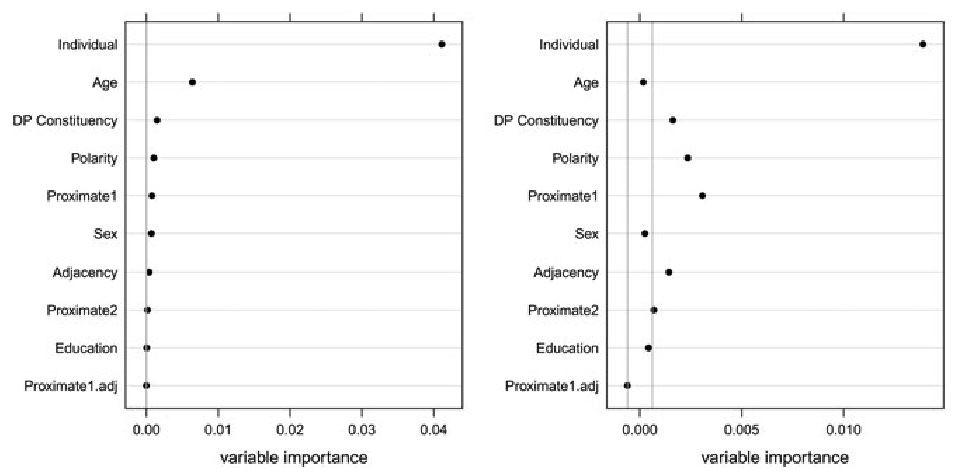
\includegraphics[width = 0.9\linewidth]{images/TagliamonteBaayen_vip.png}
    \caption{Variable importance plot from \citet{tagliamonteModelsForestsTrees2012}. The plot on the left shows the impurity importance (i.e., Gini index) and the plot on the right shows the permutation importance. The y-axis shows the different predictors for both plots.}
    \label{fig:tagliamonte_importance}
\end{figure}

By looking at both the impurity importance and the permutation importance, we can get a better understanding of which predictors are the most important in making the splits in the space. For \citet{tagliamonteModelsForestsTrees2012} this meant that the Individual variable was the most important predictor in making the splits in the data. The other predictors were also important but we now see differences between the two plots in which are important. In general, the researcher should look at both the impurity importance and the permutation importance to gain an understanding of which predictors are the most important in making the splits in the data. If there is a overlap between the two plots, then we can be more confident that the predictor is important in making the splits in the data. If there is a large difference between the importance of a predictor, then we should be cautious in that predictor's importance. 

%--------------------------
\section{Random Forests in SLZ} \label{sec:bagging_slz}
%--------------------------
%--------------------------------------------------------------------------
\subsection{Data processing} \label{sec:bagging:processing}
%--------------------------------------------------------------------------
Data points with an absolute z-score value greater than 3 were considered outliers and excluded from the analyses. Within each vowel category, we calculated the Mahalanobis distance in the F1-F2 panel. Each data point with a Mahalanobis distance greater than 6 was considered an outlier and excluded from the analysis. Using the Mahalanobis distance allows me to compare the data points to the mean of the F1-F2 panel for each vowel category. The larger the Mahalanobis distance is the more deviant the data point is from the mean which in turn indicated that the data point was improperly tracked. This is comparable to what was done in \citet{seyfarthPlosiveVoicingAcoustics2018,chaiCheckedSyllablesChecked2022,garellekPhoneticsWhiteHmong2023}.  

Energy was excluded if it had a zero value and then logarithmically transformed to normalize its right-skewed distribution. Afterward, the resulting logarithmically transformed data was z-scored, and any data point with a z-score greater than three was excluded. Additionally, residual H1* was calculated and included in the analysis.

Once these steps were completed, the mean of each vowel and speaker for the fourth through seventh intervals was taken. This is similar to what \citet{keatingCrosslanguageAcousticSpace2023} did by taking the middle of the vowel for their analysis. This choice minimizes the effect of the onset and offset of the vowel on the acoustic measures, which are more likely to be affected by the surrounding consonants and should give us the most accurate representation of the vowel quality. Because z-scores were used, this resulted in negative measures. To correct for this, I added the absolute value of the minimum z-score to each measure. This results in a dataset that still preserves the relative differences in the scores while providing a dataset that is was positive for the MDS analysis.

%--------------------------------------------------------------------------

Using this data, I will use bagging trees to understand the importance of the different acoustic measures in making the splits in the acoustic space of SLZ. In order to determine the number of trees that are needed to stabilize the prediction, I compared models with different numbers of trees. The results of this comparison are shown in Figure~\ref{fig:bagging_tree}. The x-axis shows the number of trees that were used in the model and the y-axis shows the out-of-bag error. The out-of-bag error is a measure of how well the model predicts the data that was not used to train the model. The lower the out-of-bag error, the better the model is at predicting unseen data.

\begin{figure}[!ht]
    \centering
    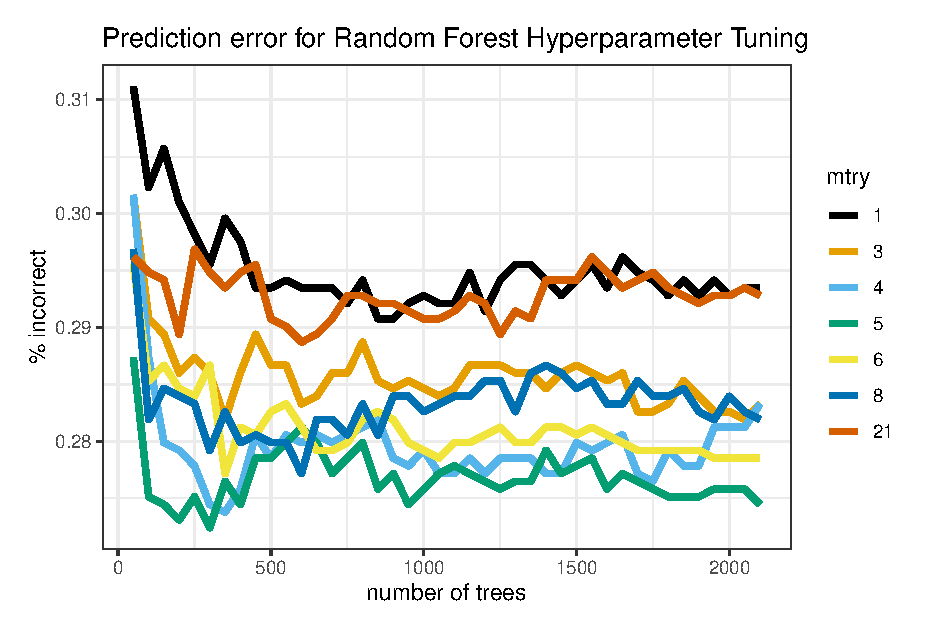
\includegraphics[width = 0.9\linewidth]{images/RandomForest/tree_num_dur.eps}
    \caption{Plot showing the percent of inaccurately classified phonation types as a function of the number of trees ran. The different colored lines indicate the different mtry values.}
    \label{fig:bagging_tree}
\end{figure}

From Figure~\ref{fig:bagging_tree}, it is clear that the out-of-bag error stabilizes at approximately 1400 trees after which the out-of-bag error increases and decreases while hovering around an out-of-bag error rate of 0.305. This means that the number of trees that are required for the the bagging model to be the most stable is 1400 trees. In order to further insure the stability of the model, I also ran a 10-fold cross-validation on the bagging model with 1400 trees. The results of this model are shown in Figure~\ref{fig:bagging_importance}. In interpreting the variable importance plot we arrange the variables by their importance in making the splits in the data. The x-axis shows the mean decrease in Gini index, which is a measure of impurity, for each predictor and the y-axis shows the different predictors that were used in the model. Typically, the top 3-5 predictors are the most important in making the splits in the data \citep{boehmkeHandsOnMachineLearning2019}.

\begin{figure}[!ht]
    \centering
    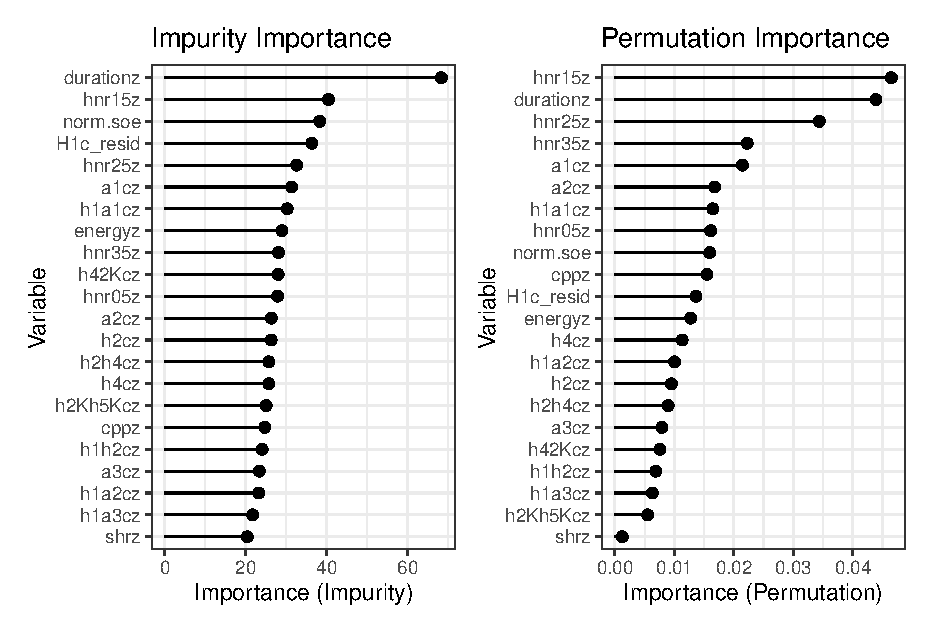
\includegraphics[width = \linewidth]{images/RandomForest/rf_dur_plots.eps}
    \caption{Variable importance plots showing the impurity importance and permutation importance of each acoustic measure.}
    \label{fig:bagging_importance}
\end{figure}

From Figure~\ref{fig:bagging_importance}, the predictors with the largest mean decrease in Gini index are A1* (the amplitude of the harmonic closest to the first formant), residual H1*, and the harmonics-to-noise ratio over the frequency range from 0 Hz to 1500 Hz (HNR 1500 Hz). This means that these three predictors are the most important in making the splits in the acoustic space of SLZ. This is consistent with the results of the MDS analysis in Chapter~\ref{ch:acousticlandscape}, where these three predictors were some of the predictors that contributed the most to the different dimensions of the acoustic space. 

%--------------------------
\section{Discussion of the bagging results} \label{sec:bagging_discussion}
%--------------------------

It is interesting to not that in both the MDS analysis and the bagging trees, the same three predictors are found to play a role in the acoustic space of SLZ. These two analyses complement each other and help us to better understand what measures to focus are attention on. From Chapter~\ref{ch:acousticlandscape}, we saw that the acoustic measure A1* was heavily weighted for both dimensions 1 and 2. It is not surprising then that this measure would rank so high in the variable importance.

The other two measures that the bagging analysis found to be of most importance are the measures residual H1* and HNR 1500 Hz. These two measures were also important for the analysis in Chapter~\ref{ch:acousticlandscape}. However, they were only heavily weighted for dimension 3. 

The rest of this section will discuss each of the measures that were found to be important in the bagging analysis and how they relate to the different voice qualities in SLZ and other linguistic phenomena. 

%--------------------------
\subsection{Importance of A1*} \label{sec:bagging_a1}
%--------------------------

The measure that was found to be the most important for classifying SLZ's phonation contrasts was A1*. This measure captures the amplitude of the harmonic closest to the first formant. This measure is typically not found in voice quality research except as a way to normalize the amplitude of the first harmonic (i.e., H1*). This goes back to \citet{fischer-jorgensenPhoneticAnalysisBreathy1968} who used this as one of the ways to correct for the high pass filtering, in addition to the widely used H1*$-$H2* measure. However, A1* as a standalone measure is not typically used in voice quality research. Therefore what we are to make of this measure's importance in SLZ is not clear as is its behavior in regards to the different phonations. 

When we look at how A1* is distributed across the different voice qualities in SLZ, as seen as Figure~\ref{fig:a1}, we see that modal vowels are found at the top of the chart with the other phonation contrasts located lower on the chart. The phonation that is found at the bottom of the chart is breathy voice. 
\begin{figure}[!ht]
    \centering
    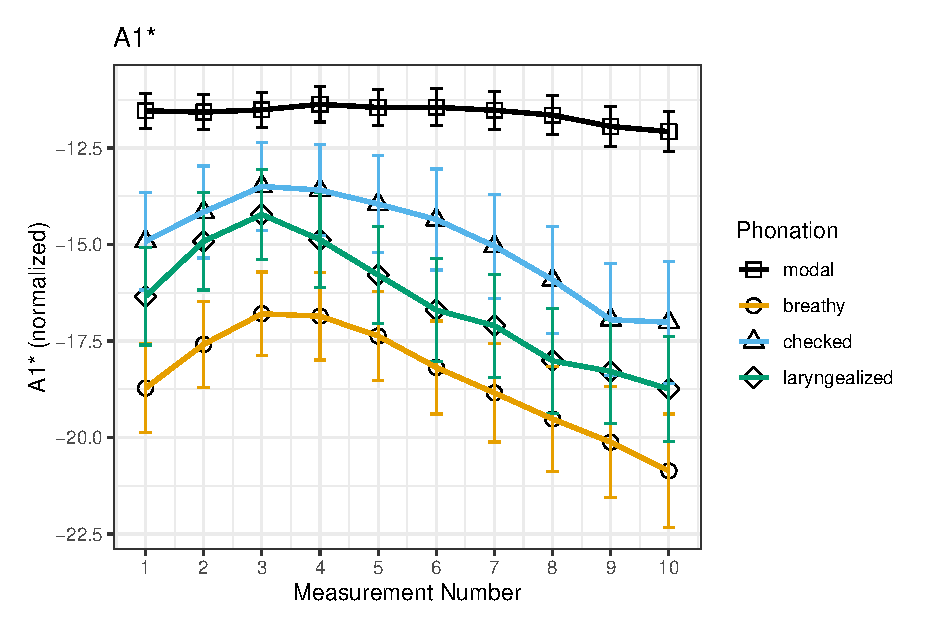
\includegraphics[width = 0.9\linewidth]{images/slz_a1c.eps}
    \caption{Plot showing the distribution of A1* across the different voice qualities in SLZ.}
    \label{fig:a1}
\end{figure}

The pattern of behavior for A1* is very similar to what is found in descriptions of the behavior of the frequency of F1 in breathy voice contexts. For example differences in the frequency of F1 are typically used to distinguish register differences in Southeast Asian languages \citep{brunelleRegisterEasternCham2005,brunelleDialectExperiencePerceptual2012,brunelleTonePhonationSoutheast2016}.

As described in \citet{brunelleTonePhonationSoutheast2016}, many of the languages of Southeast Asia have what is called register. The linguistic term register is defined as ``the redundant use of pitch, voice quality, vowel quality, and durational differences to distinguish (typically two) contrastive categories'' \citep[193]{brunelleTonePhonationSoutheast2016}, and was first used by \citet{hendersonMainFeaturesCambodian1952} to describe the categorical contrasts found in Khmer. The characteristics that define the higher and lower registers are found in Table~\ref{tab:register_correlates}.

\begin{table}[!ht]
    \centering
    \caption{Possible phonetic correlates of register. From \citet{brunelleTonePhonationSoutheast2016}.}
    \label{tab:register_correlates}
    \begin{tabular}{ll}
        \lsptoprule
        \textbf{Higher Register} & \textbf{Lower Register} \\
        \hline
        Higher pitch & Lower pitch \\
        Tense/Modal voice & Lax/Breathy voice \\
        Monophthongs/shorter vowels & Diphthongs/longer vowels \\
        Raised F1/lower vowels/[+ATR] & Lowered F1/higher vowels/[-ATR] \\
        Plain stops/shorter VOT & Aspirated stops/longer VOT \\
        \lspbottomrule
    \end{tabular}
\end{table}

From this table, the lower register is what interests us here. The lower register is associated with breathy voice and a lowered first formant. There is evidence that breathy voice frequently has a lower first formant than modal voice in paralinguistic settings for English \citep{lottoEffectVoiceQuality1997}.  However, these studies do not discuss the amplitude of the first formant but rather the frequency of the first formant.

Another comparison can be found in nasality research, where this measure is discussed quite extensively either alone or in association with the nasal pole (e.g., \cite{chenAcousticCorrelatesEnglish1997,delvauxPerceptionContrasteNasalite2009,macmillanIntegralityNasalizationF11999,pruthiAcousticParametersAutomatic2004,,schwartzAcousticsNormalNasal1968,stevensAcousticPhonetics2000,stylerAcousticalPerceptualFeatures2015,stylerAcousticalFeaturesVowel2017}). These studies discuss how in nasalized contexts the amplitude of the first formant is typically found to be lower than in oral ones, again similar to what we see in Figure~\ref{fig:a1}.

There is a large body of research that discusses that nasality is closely associated with breathy voice or the glottal consonants, in a phenomenon called \textit{rhinoglottophilia} \citep{matisoffRhinoglottophiliaMysteriousConnection1975,ohalaPhoneticExplanationsNasal1975,ohalaPhoneticsNasalPhonology1993,bennettMayanPhonology2016}. In \citet{blevinsEvolutionPonapeicNasal1993,matisoffRhinoglottophiliaMysteriousConnection1975}, this association is attributed to the acoustic and perceptual similarities between nasalization and breathy voice. In one study, \citet{garellekBreathyVoiceNasality2016} showed that in nasalization in three different Yi languages were associated with breathy voice. Leading the authors to suggest that breathy voice during nasalization can arise from misperception or as a type of phonetic enhancement. 

In regards to what is going on in SLZ, it is not clear if the lowering of A1* for breathy voice can be attributed to the same observations as discussed above. I suggest there are three different possibilities to explain what is going on in SLZ. First; because SLZ does not have phonemic nasaliZation, it is possible that speakers of SLZ are using nasalization as a way to phonetically enhance the the contrast of breathy voice. Essentially, the reverse of what was reported by \citet{garellekBreathyVoiceNasality2016}. This possibility could be tested acoustically by performing an experiment to detect nasal airflow during breathy vowels. The second possibility is that the same measures that work for detecting nasality can also be used to detect breathy voice. This second possibility could be easily tested by examining whether A1* and the other measures for nasality work in other breathy voice contexts cross-linguistically. The third possibility is that the lowering of A1* is a result of sub-glottal resonances which is much harder to test than the other two possibilities. 

% \begin{figure}[htbp]
%     \centering
%     \includegraphics[width = \linewidth]{images/test.eps}
%     \caption{<caption>}
%     \label{<label>}
% \end{figure}
%--------------------------
\subsection{Importance of Residual H1*} \label{sec:bagging_residual}
%--------------------------
As residual H1* is a type of spectral slope measure it is expected to show similar behavior to other spectral slope measures. Namely, breathy voice should be associated with a higher score than modal voice. Since the two types of laryngealization are closely associated with creaky voice, they should be associated with a lower score than modal voice. Additionally, there is a temporal difference between the two types of laryngealization, it is expected that checked voice will have a lower score toward the end of the vowel and  rearticulated voice will have a lower score in the middle of the vowel. 

In Figure~\ref{fig:residualH1}, we see that are predictions are correct. Breathy voice is associated with a higher score than modal voice. The two types of laryngealization are associated with a lower score than modal voice.

\begin{figure}[!ht]
    \centering
    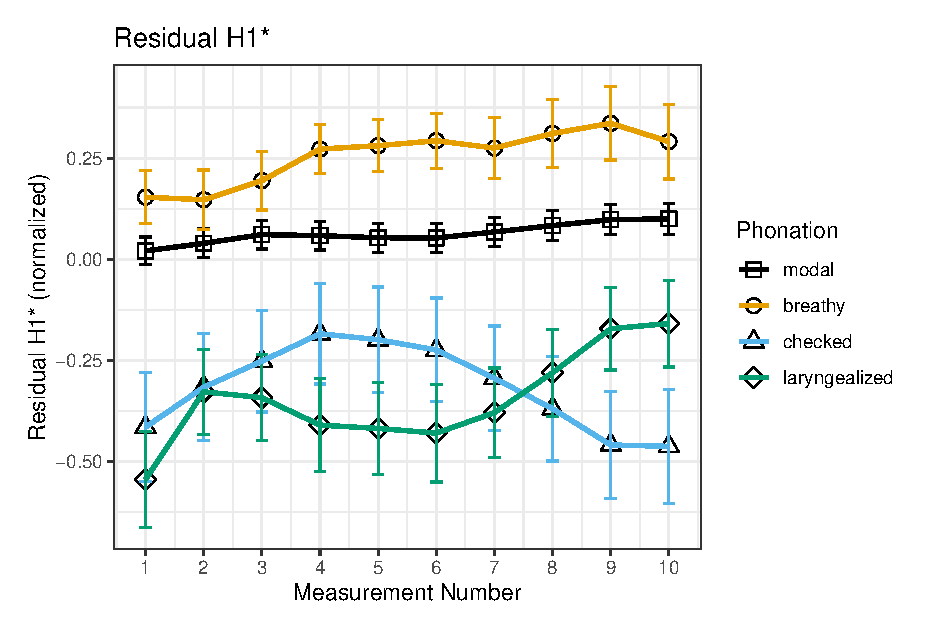
\includegraphics[width = 0.9\linewidth]{images/slz_residual_h1c.eps}
    \caption{Plot showing the distribution of residual H1* across the different voice qualities in SLZ.}
    \label{fig:residualH1}
\end{figure}

A further analysis of the results of this measure using generalized additive (mixed) models (GAM(M)s; \cite{hastieGeneralizedAdditiveModels1986,woodGeneralizedAdditiveModels2017,soskuthyGeneralisedAdditiveMixed2017,wielingAnalyzingDynamicPhonetic2018}) shows that the temporal behavior of the two types of laryngealization is also correct. Checked voice is associated with a lower score toward the end of the vowel and rearticulated voice is associated with a lower score in the middle of the vowel. Additionally, the results of the GAMM show that for the first three time points there is no significant difference between breathy and modal voice. Suggesting that breathy voice is more closely associated with the latter part of the vowel than the beginning. The full results of the GAMM for residual H1* are discussed in Chapter~\ref{ch:residual_h1}.

%--------------------------
\subsection{Importance of the HNR \textless 1500 Hz} \label{sec:bagging_hnr}
%--------------------------

The acoustic measure HNR $<$ 1500 Hz is a harmonics-to-noise ratio measure that is calculated over the frequency range from 0 Hz to 1500 Hz and is a measure of the amount of noise in the signal or in other words it is measure of periodicity. In these measures, modal voice is associated with a higher score than non-modal phonations. This is because modal voice is associated with a higher degree of periodicity than non-modal phonations as a-periodicity is a defining feature of non-modal phonations (e.g., \cite{hillenbrandAcousticCorrelatesBreathy1996,blankenshipTimeCourseBreathiness1997,kentVoiceQualityMeasurement1999}).

As seen in Figure~\ref{fig:hnr1500}, this is exactly what we see in SLZ. Modal voice is associated with a higher score than non-modal phonations. Among the non-modal phonations, breathy and rearticulated voice have a higher HNR $<$ 1500 Hz than checked voice. 

\begin{figure}[!ht]
    \centering
    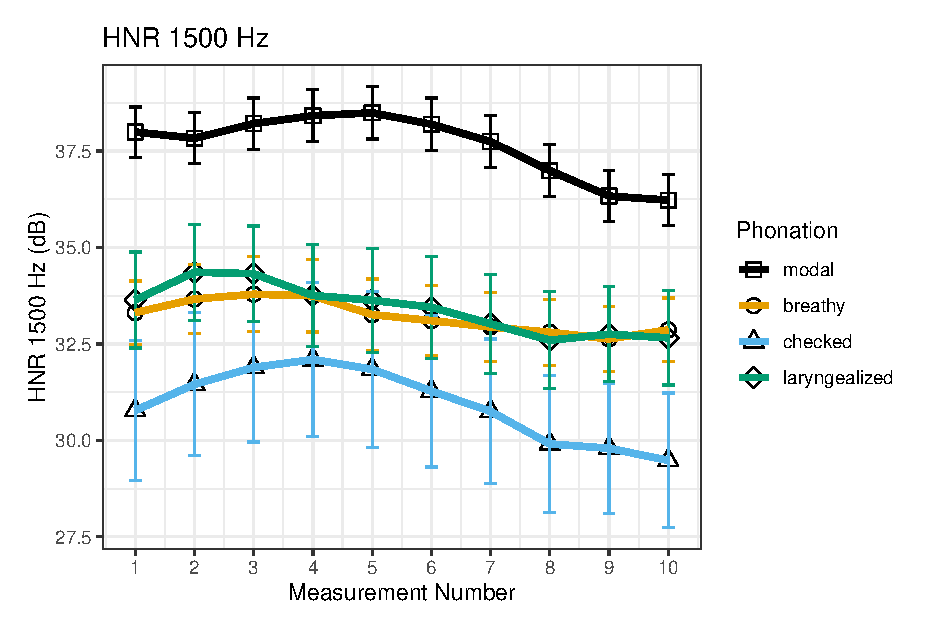
\includegraphics[width = 0.9\linewidth]{images/slz_hnr15.eps}
    \caption{Plot showing the distribution of HNR $<$ 1500 Hz across the different voice qualities in SLZ.}
    \label{fig:hnr1500}
\end{figure}

The fact that breathy and rearticulated voice have a higher HNR $<$ 1500 Hz than checked voice is not surprising. As discussed in Chapter~\ref{ch:SLZ}, breathy and rearticulated voices are associated with more modal-like qualities than checked voice. In most instances of rearticulated voice, the vowel is produced with modal voice except for a small portion of the middle of the vowel where the vowel is produced with creaky voice or a glottal occlusion. Breathy voice typically appears  very periodic but with a high degree of noise in the signal. Checked voice on the other hand is typically the shortest of the non-modal phonations and is associated with a high degree of aperiodicity in the signal from the creaky voice that is produced at the end of the vowel. This is why checked voice has the lowest HNR $<$ 1500 Hz of the non-modal phonations.

This measure will be very important in Chapter~\ref{ch:testing_lc}, where this measure will be used to test the predictions of the laryngeal complexity hypothesis.

%--------------------------
\section{Conclusion} \label{sec:bagging_conclusion}
%--------------------------

In conclusion, the results of the bagging analysis show that the acoustic measures A1*, residual H1*, and HNR $<$ 1500 Hz are the most important in making the splits in the acoustic space of SLZ. These three measures are also the measures that were found to be the important in the MDS analysis in Chapter~\ref{ch:acousticlandscape}. This suggests that these three measures play an important role in defining and characterizing the different voice qualities from one another in SLZ. 


%--------------------------------------------------------------------------
\chapter{Testing laryngeal complexity in SLZ} \label{ch:testing_lc}
%--------------------------------------------------------------------------

%--------------------------------------------------------------------------
\section{Introduction}\label{sec:introduction_of_lc}
%--------------------------------------------------------------------------

This chapter investigates the role that laryngeal complexity plays in Santiago Laxopa Zapotec. Laryngeal complexity is used to describe the contrastive use of tone and phonation in many languages, especially in the Oto-Manguean languages \citep{blankenshipTimeCourseBreathiness1997,blankenshipTimingNonmodalPhonation2002,silvermanLaryngealComplexityOtomanguean1997,silvermanPhasingRecoverability1997}. As mentioned in Chapter~\ref{ch:SLZ}, SLZ is a laryngeally complex language, because of its contrastive use of both tone and phonation. This means that SLZ can be used to test the predictions of laryngeal complexity, with respect to the phasing and recoverability of tone and phonation.

The goal of this chapter is to show that laryngeal complexity is present in SLZ as evidenced by the phasing of nonmodal phonation in several acoustic measures. This is done by looking at the acoustic properties of SLZ phonation using a combination of Strength of Excitation (SoE), Harmonic-to-Noise Ratio (HNR) < 1500 Hz and \textit{f}0 perturbations. It will be shown that there is a clear phasing between modal and nonmodal phonation in vowels that are described as breathy, checked, and rearticulated. 

These measures were selected based on the results of the MDS analysis in Chapter~\ref{ch:acousticlandscape} and the Random Forest analysis in Chapter~\ref{ch:revealing_trees}. Both MDS and Random Forest analyses showed that SoE and HNR < 1500 Hz were the most important measures to distinguish between the different types of phonation. SoE has previously been used to show that there is a clear phasing between modal and rearticulated vowels in San Sebastián del Monte Mixtec \citep{wellerInteractionsToneGlottalization2023,wellerLexicalToneVowel2023,wellerVoiceQualityTone2024}. 

HNR < 1500 Hz has not been used to date to show phasing between modal and nonmodal phonation. As a harmonics-to-noise ratio measure, HNR < 1500 Hz is a measure of the noise in the signal. This means that it can be used to determine if there is aperiodicity in the signal, which is one of the defining characteristics of nonmodal phonation \citep{ladefogedSoundsWorldsLanguages1996}. This means that HNR < 1500 Hz can be used to determine if there is a clear phasing between modal and nonmodal phonation in these vowels. 

Additionally, \textit{f}0 perturbation has been used previously to show that there is phasing between modal and nonmodal phonation in several Oto-Manguean languages \citep{garellekAcousticConsequencesPhonation2011,dicanioCoarticulationToneGlottal2012,keltererPhonationTypeContrasts2020}. 

The remainder of this chapter will be organized as follows. First, in Section~\ref{sec:what_is_lc}, I will provide a brief overview of laryngeal complexity and phasing and recoverability of tone and phonation in Section~\ref{sec:what_is_lc}. In Section~\ref{sec:previous_analyses} I will discuss previous analyses of laryngeal complexity. In Section~\ref{sec:analysis_of_lc} I will discuss the methods used to analyze laryngeal complexity in SLZ. In Section~\ref{sec:results_of_lc} I will present the results of the analysis. Finally, in Section~\ref{sec:discussion_of_lc} I will discuss the implications of these results for our understanding of laryngeal complexity in SLZ.

%--------------------------------------------------------------------------
\section{What is Laryngeal Complexity?}\label{sec:what_is_lc}
%--------------------------------------------------------------------------

Laryngeal complexity is defined as the contrastive use of tone and phonation within the same syllablic nucleus \citep{blankenshipTimeCourseBreathiness1997,blankenshipTimingNonmodalPhonation2002,silvermanLaryngealComplexityOtomanguean1997,silvermanPhasingRecoverability1997}. This use of contrastive tone and phonation is one of the defining characteristics of the Oto-Manguean languages \citep{silvermanLaryngealComplexityOtomanguean1997}. However, it is not limited to just these languages. It has also been used to describe the behavior of tone or pitch in languages outside of the Oto-Manguean languages; such as the Tibeto-Burman languages of Mpi and Tamang \citep{silvermanLaryngealComplexityOtomanguean1997,silvermanPhasingRecoverability1997}, the Mayan language Yucatec Mayan \citep{frazierPhoneticsYucatecMaya2013}, and to describe the behavior of coarticulatory pitch and phonation in the Germanic language Danish \citep{frazierPhoneticsYucatecMaya2013,penaStodTimingDomain2022,penaProductionPerceptionStod2024}.

According to \citet{silvermanLaryngealComplexityOtomanguean1997,silvermanPhasingRecoverability1997}, even though tone and phonation are apparently allowed to co-occur in the same syllabic nucleus they are not allowed to be realized at the same time. \citeauthor{silvermanLaryngealComplexityOtomanguean1997} argues that this is because they are in competition with one another over the same articulatory gestures and perceptual resources. This means that tone and phonation must be realized in a temporally ordered fashion. This is what \citeauthor{silvermanLaryngealComplexityOtomanguean1997} refers to as phasing. Phasing is the idea that the two components of laryngeal complexity, tone and phonation, are temporally ordered with respect to one another. This means that one portion of the vowel is realized with modal phonation with the acoustic correlates of tone and the other portion of the vowel is realized with non-modal phonation with the acoustic correlates of said phonation. This phasing is also closely linked to the second main concept of laryngeal complexity, recoverability. Recoverability is the idea that the listener must be able to recover the underlying phonation and tone from the signal. These two concepts will be discussed in more detail in Section~\ref{sec:phasing_and_recoverability}.

%--------------------------------------------------------------------------
\subsection{Phasing and recoverability}\label{sec:phasing_and_recoverability}
%--------------------------------------------------------------------------

According to \citet{silvermanLaryngealComplexityOtomanguean1997,silvermanPhasingRecoverability1997}, one of the defining aspects of laryngeal complexity is the concept of phasing and recoverability. Under this idea, in laryngeally complex vowels the phonation and tone are phased with respect to one another in way that lends itself to a listener's ability to recover the underlying phonation and tone. In practical terms this means that laryngeally complex vowels are composed of two components: a modal voice portion of the vowel where tone is realized, and a non-modal voice portion of the vowel where phonation is realized. For the researcher that means that there are two distinct portions of the vowel that can be analyzed separately and that need to be analyzed temporally rather than spectrally \citep[237]{silvermanLaryngealComplexityOtomanguean1997}.

For example, in the Oto-Manguean language Jalapa Mazatec, breathiness or creakiness is realized only on the first portion of the vowel either as full laryngeal consonant or as a laryngeal feature on the vowel \citep[238]{silvermanLaryngealComplexityOtomanguean1997}. The second portion of the vowel is realized as a modal voice vowel with one of the three tones belonging to the tonemes of the language. This means that the breathiness or creakiness is phased with respect to the tone.

\citeauthor{silvermanLaryngealComplexityOtomanguean1997} argues that there are three principles that help explain why laryngeal complexity needs to be temporally ordered or phased: (i) sufficient acoustic distance, (ii) sufficient articulatory compatibility, and (iii) optimal auditory salience. 

%--------------------------------------------------------------------------
\subsubsection{Sufficient acoustic distance}\label{sec:sufficient_acoustic_distance}
%--------------------------------------------------------------------------

\citet{silvermanLaryngealComplexityOtomanguean1997} argues that sufficient acoustic distance is necessary for the recoverability of the phonation and tone. As Silverman explain, listeners do not rely on the fundamental frequency alone to perceive pitch. Instead, listeners use the harmonic spacing and the pulse period in the signal to perceive pitch \citep{ritsmaFrequenciesDominantPerception1967,remezIntonationSinusoidalSentences1993}. For modal phonation, this means that the harmonic spacing and pulse periods are present and encode a salient pitch value. However, during non-modal phonation, the harmonic spacing and pulse periods are often obscured or not present.

For breathy voice, this means that there is a general weakening 
of the harmonic structure which makes it difficult to recover the pitch by the listener \citep{silvermanPhasingRecoverability1997}. Creaky voice on the other had obscures the pulse periods due to its aperiodic and unstable glottal vibration \citep{ladefogedSoundsWorldsLanguages1996}. This is what was observed in Mazatec where the harmonic structure is gone and the pulses are indiscernible \citep{kirkQuantifyingAcousticProperties1993}. Additionally, the perception of pitch is rendered indiscernible when the pulse periods are varied by 10\% or more \citep{rosenbergPitchDiscriminationJittered1966}.

These observations lead \citet{silvermanLaryngealComplexityOtomanguean1997} to conclude that if a period glottal wave is either obscured (as with breathy voice) or not present (as with creaky voice), the acoustic signal cannot encode a salient pitch value. This means that the phonation and tone must be phased with respect to one another in order for the listener to recover the underlying phonation and tone. I will return to this point in Section~\ref{sec:discussion_of_lc}.

%--------------------------------------------------------------------------
\subsubsection{Sufficient articulatory compatibility}\label{sec:sufficient_articulatory_compatibility}
%--------------------------------------------------------------------------

Another important point for the \citeauthor{silvermanLaryngealComplexityOtomanguean1997}'s theory about laryngeal complexity has to deal with the articulatory compatibility of the phonation and tone. One of the guiding ideas behind this principle is that there is a principle of least effort in biological motor systems such as with speech production \citep{lindblomEconomySpeechGestures1983}. According to \citet{lindblomEconomySpeechGestures1983}, speech gestures can be thought of as distinct motor goals in our speech production system. These goals are achieved by the speaker through the coordination of the articulators with the least amount of effort. This means that that the gestures are coordinated in such a way that they are compatible with one another. This manifests itself either through sequencing or coarticulation of the gestures.

A good example of this comes from nasalization. In nasal contexts, the velum is lowered to allow air to pass through the nasal cavity, creating a nasal sound. This velum lowering gesture is compatible with the gestures needed in the oral cavity to produce different vowel qualities. This is what leads to the production of nasal vowels in languages like French or Portuguese. Additionally, this lowering also occurs in languages that do not have contrastive nasal vowels, such as English, where the velum is lowered in anticipation of a nasal consonant. This lowering of the velum is compatible with the gestures needed to produce the vowels in the oral cavity \citep[e.g.,][]{ohalaPhoneticExplanationsNasal1975,chenAcousticCorrelatesEnglish1997,stylerAcousticalPerceptualFeatures2015}.

According to \citeauthor{silvermanLaryngealComplexityOtomanguean1997}'s theory of laryngeal complexity, this idea of articulatory compatibility is also driving the need to phase phonation and tone. In the case of laryngeal complexity this is because it is assumed that both tone and phonation are produced by the larynx, more specifically the vocal folds and the glottis. This comes from early work on phonation and tone. For tone, \citet{ohalaProductionTone1978} showed that pitch was controlled primarily by the tensing or laxing of the vocal folds which changed the rate at which the vocal folds vibrate. For phonation, it was similarly shown that the amount the vocal folds where held open or closed determined the type of phonation that was produced \citep{ladefogedSoundsWorldsLanguages1996}. This aspect of phonation was shown in Figure~\ref{fig:phonation_types} and repeated here as Figure~\ref{fig:phonation_types_repeat}. 

\begin{figure}[h!]
    \centering
    \begin{tikzpicture}
        % Draw the line with arrows at both ends
        \draw[<->, line width=0.5mm] (0,0) -- (10,0);
        
        % Labels underneath the line
        \node[below] at (0,0) {[h]};
        \node[below] at (2,0) {Breathy};
        \node[below] at (5,0) {Modal};
        \node[below] at (8,0) {Creaky};
        \node[below] at (10,0) {[ʔ]};
        
        % Labels above the line
        \node[above] at (0,0) {Open Glottis};
        \node[above] at (10,0) {Closed Glottis};
    \end{tikzpicture}
    \caption{A diagram showing the relationship between breathy, modal, and creaky phonation types. Based on \citet{gordonPhonationTypesCrosslinguistic2001}.}
    \label{fig:phonation_types_repeat}
\end{figure}

For \citeauthor{silvermanLaryngealComplexityOtomanguean1997}'s \citeyear{silvermanLaryngealComplexityOtomanguean1997} theory of laryngeal complexity, the articulatory mechanisms for tone and phonation are exactly the same which leads to a need to phase the two in order to optimally make use of the same articulatory gestures. However, there is a growing body of literature that shows that tone and phonation is much more complex and is reliant on the entire larynx not just the vocal folds (e.g., \cite{eslingVoiceQualityLaryngeal2019}). This matter will be picked up again in Section~\ref{sec:discussion_of_lc}.

%--------------------------------------------------------------------------
\subsubsection{Optimal auditory salience}\label{sec:optimal_auditory_salience}
%--------------------------------------------------------------------------

The last important point for \citeauthor{silvermanLaryngealComplexityOtomanguean1997}'s theory of laryngeal complexity is the idea of optimal auditory salience. Research into the behavior of nerve responses to acoustic signals has shown that the auditory system is sometimes more and other times less recoverable depending on the signal, which led \citet{bladonPhoneticsHearers1986} to proposes two major principles for auditory phonetics: (i) the on/off response asymmetry and (ii) short-term adaptation.

The on/off response asymmetry principle has origins in the work of \citet{tylerPsychoacousticPhoneticTemporal1982}. This principle states ``spectral changes whose response in the auditory nerve is predominantly an onset of firing are much more perceptually salient than those producing an offset. \citep[249]{silvermanLaryngealComplexityOtomanguean1997}''. This means that changes in the signal that cause an increase in the firing rate in the auditory nerve are easier to perceive when this firing starts compared to when it ends. 

The second principle, short-term adaptation, states that ``after a rapid onset of auditory nerve discharge at a particular frequency, there is a decay to a moderate level of discharge, even though the same speech sound is continuing to be produced \citep[250]{silvermanLaryngealComplexityOtomanguean1997}'' and is based on the work of \citet{delgutteCorrelatesPhoneticDistinctions1982}. This means that the auditory nerve is less sensitive to changes in the signal after a rapid onset of firing which in turn means that the auditory nerve is less able to recover the underlying phonation and tone when the signal is not changing.

For \citeauthor{silvermanLaryngealComplexityOtomanguean1997}, these two principles are important because they help to provide an acoustic explanation for why laryngeal complexity needs to be phased. By phasing tone and phonation, the listener is able to recover the signal more easily. This is because when there is a change in the signal the auditory nerve has the greatest chance of recovering the signal. In regards to tone and phonation, this means that when there is a change from tone's modal phonation to nonmodal phonation or from nonmodal phonation to tone's modal phonation, the listener is able to perceive the difference better than if the two were produced simultaneously. Additionally, these two principles suggest that some phasing relationships are more perceptually saliant than others. Based on these two principles things are easier to perceive if they are produced first or if there is a large change in the signal. 

To illustrate this point graphically, \citeauthor{silvermanLaryngealComplexityOtomanguean1997} provides a series of figures that show the relationship between the articulatory, acoustic, and perceptual components of laryngeal complexity. These figures are shown in Figures~\ref{fig:silverman_18}, \ref{fig:silverman_19}, and \ref{fig:silverman_20}. 

Figure~\ref{fig:silverman_18} shows the characteristics for the sequence of [ha˥], where breathiness is produced first followed by a modal vowel with high tone. The figure shows that when the breathiness is produced first, the auditory nerve response is high followed by a sharp decline through the rest of the breathiness. As the energy increases when the modal vowel with high tone is produced there is a sharp increase in the auditory nerve response which is followed by a gradual decline. This means that it is easier for the listener to perceive the transition and recover the underlying phonation and tone.
\begin{figure}[h!]
    \centering
    \begin{tikzpicture}[x=3.5cm, y=1cm]

        % Axis Labels
        \node[anchor=east] at (-0.1,5) {\textit{articulatory}};
        \node[anchor=east] at (-0.1,4.5) {\textit{supralaryngeal:}};
        \node[anchor=east] at (-0.1,4) {\textit{laryngeal:}};
        \node[anchor=east] at (-0.1,3) {acoustic signal};
        \node[anchor=east] at (-0.1,2.6) {(amplitude)};
        \node[anchor=east] at (-0.1,2) {auditory nerve};
        \node[anchor=east] at (-0.1,1.6) {response at CF};
        \node[anchor=east] at (-0.1,0.5) {percept};
        
        % Articulatory Supralaryngeal
        \node at (0.5,4.5) {vowel};
        
        % Articulatory Laryngeal
        \node at (0.5,4) {abduction};
        \node at (1.5,4) {approximation tensing};
        
        % Acoustic signal (amplitude)
        \draw[thick] (0,2.5) -- (1,2.5) -- (1,3) -- (2,3);
        
        % Auditory nerve response
        \draw[thick] (0,2) -- (0.25,1.4) -- (1,1.4) -- (1,2) -- (1.25,1.75) -- (2, 1.75);
        
        % Percept
        \node at (0.5,0.5) {h};
        \node at (1.5,0.5) {a˥};
        
        \end{tikzpicture}
    \caption{Schematic representation of the characteristics of [ha˥] sequences. Adaptation of figure from \citet{silvermanLaryngealComplexityOtomanguean1997}.}
    \label{fig:silverman_18}
\end{figure}

For Figure~\ref{fig:silverman_19}, the sequence is reversed. In this case, the modal vowel with high tone is produced first followed by breathiness. The figure shows that when the modal vowel with high tone is produced first, the auditory nerve response is at its highest followed by a sharp decline through the rest of the modal vowel portion. Because there is no energy increase associated with breathiness there is a continual decrease in the auditory nerve response. This means that it is not as easy as prevocalic  of for the listener to perceive the transitions and recover the underlying phonation and tone.
\begin{figure}[h!]
    \centering
    \begin{tikzpicture}[x=3.5cm, y=1cm]

        % Axis Labels
        \node[anchor=east] at (-0.1,5) {\textit{articulatory}};
        \node[anchor=east] at (-0.1,4.5) {\textit{supralaryngeal:}};
        \node[anchor=east] at (-0.1,4) {\textit{laryngeal:}};
        \node[anchor=east] at (-0.1,3) {acoustic signal};
        \node[anchor=east] at (-0.1,2.6) {(amplitude)};
        \node[anchor=east] at (-0.1,2) {auditory nerve};
        \node[anchor=east] at (-0.1,1.6) {response at CF};
        \node[anchor=east] at (-0.1,0.5) {percept};
        
        % Articulatory Supralaryngeal
        \node at (0.5,4.5) {vowel};
        
        % Articulatory Laryngeal
        \node at (0.5,4) {approximation tensing};
        \node at (1.5,4) {abduction};
        
        % Acoustic signal (amplitude)
        \draw[thick] (0,3) -- (1,3) -- (1,2.5) -- (2,2.5);
        
        % Auditory nerve response
        \draw[thick] (0,2) -- (0.25,1.5) -- (1,1.5) -- (1.25,1) -- (2,1);
        
        % Percept
        \node at (0.5,0.5) {a˥};
        \node at (1.5,0.5) {h};
        
        \end{tikzpicture}
    \caption{Schematic representation of the characteristics of [a˥h] sequences. Adaptation of figure from \citet{silvermanLaryngealComplexityOtomanguean1997}.}
    \label{fig:silverman_19}
\end{figure}

In regards to the third type of sequence, [aha˥], the figure shows that the auditory nerve response is at its highest when the modal vowel is produced first. This is followed by a decline similar to what we see in Figure~\ref{fig:silverman_19}. However, because there is a modal vowel with high tone, we see a sharp increase in auditory nerve response. Again this is not as optimal as having the breathiness produced first. 
\begin{figure}[h!]
    \centering
    \begin{tikzpicture}[x=3.5cm, y=1cm]

        % Axis Labels
        \node[anchor=east] at (-0.1,5) {\textit{articulatory}};
        \node[anchor=east] at (-0.1,4.5) {\textit{supralaryngeal:}};
        \node[anchor=east] at (-0.1,4) {\textit{laryngeal:}};
        \node[anchor=east] at (-0.1,3) {acoustic signal};
        \node[anchor=east] at (-0.1,2.6) {(amplitude)};
        \node[anchor=east] at (-0.1,2) {auditory nerve};
        \node[anchor=east] at (-0.1,1.6) {response at CF};
        \node[anchor=east] at (-0.1,0.5) {percept};
        
        % Articulatory Supralaryngeal
        \node at (0.5,4.5) {vowel};
        
        % Articulatory Laryngeal
        \node at (0.5,4) {approximation tensing};
        \node at (1.5,4) {abduction};
        \node at (2.5,4) {approximation tensing};
        
        % Acoustic signal (amplitude)
        \draw[thick] (0,3) -- (1,3) -- (1,2.5) -- (2,2.5) -- (2,3) -- (3,3);
        
        % Auditory nerve response
        \draw[thick] (0,2) -- (0.25,1.5) -- (1,1.5) -- (1.25,1.25) -- (2,1.25) -- (2, 1.8) -- (2.25,1.5) -- (3,1.5);
        
        % Percept
        \node at (0.5,0.5) {a};
        \node at (1.5,0.5) {h};
        \node at (2.5,0.5) {a˥};
        
        \end{tikzpicture}
    \caption{Schematic representation of the characteristics of [aha˥] sequences. Adaptation of figure from \citet{silvermanLaryngealComplexityOtomanguean1997}.}
    \label{fig:silverman_20}
\end{figure}

In summary, \citeauthor{silvermanLaryngealComplexityOtomanguean1997} claims that because of this auditory response asymmetry, we see that there is a difference in the auditory nerve response depending on the sequencing of the phonation and tone. For Silverman, this implies that there is an implicational hierarchy between the different types of sequences found in laryngeal complexity. This implicational hierarchy will be discussed in more detail in Section~\ref{sec:implicational_hierarchy}.

%--------------------------------------------------------------------------
\subsection{Implicational hierarchy of laryngealization}\label{sec:implicational_hierarchy}
%--------------------------------------------------------------------------

Another aspect of \citeauthor{silvermanLaryngealComplexityOtomanguean1997}'s \citeyear{silvermanLaryngealComplexityOtomanguean1997} laryngeal complexity theory is that there is an implicational hierarchy in the phasing and ordering of phonation and tone. This hierarchy is based on how laryngealization appears in three Oto-Manguean languages. In this implicational hierarchy laryngealization can only appear in three ways: prevocalic, postvocalic, or interrupted. In the prevocalic case, the laryngealization appears before the vowel. In the postvocalic case, the laryngealization appears after the vowel. In the interrupted case, the laryngealization interrupts a vowel and appears in the middle.

According to \citet{silvermanLaryngealComplexityOtomanguean1997}, if a language has interrupted laryngealization, it must also have postvocalic laryngealization. If a language has postvocalic laryngealization, it must also have prevocalic laryngealization. In support of his claims \citet{silvermanLaryngealComplexityOtomanguean1997} provides data from three Oto-Manguean languages: Jalapa Mazatec, Comaltepec Chinantec, and Copala Trique. These languages are shown in Table~\ref{tab:implicational_hierarchy}.

\begin{table}[h!]
    \centering
    \caption{Implicational hierarchy of laryngeal complexity. The symbols h and ʔ represent laryngealization. The symbol V represents where the modal vowel is located in relation to the laryngealization.  Modified from \citet{silvermanLaryngealComplexityOtomanguean1997}.} 
    \label{tab:implicational_hierarchy}
    \begin{tabular}{lccc}
        \lsptoprule
        \textbf{Language} & \textbf{Prevocalic} & \textbf{Postvocalic} & \textbf{Interrupted} \\
        \hline 
        Jalapa Mazatec & hV˥, ʔV˥ & $-$ & $-$ \\
        Comaltepec Chinantec & hV˥, ʔV˥ & Vh˥, Vʔ˥ & $-$ \\
        Copala Trique & hV˥, ʔV˥ & Vh˥, Vʔ˥ & VhV˥, VʔV˥ \\
        \lspbottomrule
    \end{tabular}
\end{table}

For many descripitions of languages with laryngeal complexity, the implicational hierarchy seems to hold. This is certainly the case in the other Trique languages \citep{dicanioPhoneticsPhonologySan2008,dicanioItunyosoTrique2010,dicanioCoarticulationToneGlottal2012,dicanioPhoneticsFortisLenis2012,dicanioCueWeightPerception2014,dicanioGlottalTogglingItunyoso2020,elliottChicahuaxtlaTriqui2016,hollenbachPhonologyMorphologyTone1984}. However, as mentioned by \citet{frazierPhoneticsYucatecMaya2013}, it is not clear how accurate or robust this implicational hierarchy actually is. The reason for this is because it is not always clear if something is a laryngeal consonant or a laryngeal feature on the vowel. Indeed, \citet{silvermanLaryngealComplexityOtomanguean1997,silvermanPhasingRecoverability1997} treats laryngeal consonants and laryngeal features on vowels as the same thing. For example, in many of the Trique languages, the laryngealization is realized as a laryngeal consonant \citep{dicanioPhoneticsPhonologySan2008,dicanioItunyosoTrique2010,dicanioCoarticulationToneGlottal2012,dicanioPhoneticsFortisLenis2012,dicanioCueWeightPerception2014,dicanioGlottalTogglingItunyoso2020,elliottChicahuaxtlaTriqui2016,hollenbachPhonologyMorphologyTone1984}, but in Jalapa Mazatec, the laryngealization is realized as a laryngeal feature on the vowel \citep{kirkQuantifyingAcousticProperties1993,garellekAcousticConsequencesPhonation2011}. 

Another issue with the implicational hierarchy is that it is based on only three languages. This is a rather small sample size and doesn't capture the full range of variation in the Oto-Manguean languages. For example, in many Mixtec languages, laryngealization is understood to be a feature of the vowel rather than a consonant \citep[e.g.,][]{cortesSanSebastianMonte2023,eischensTonePhonationPhonologyPhonetics2022,gerfenPhonologyPhoneticsCoatzospan1999,gerfenProductionPerceptionLaryngealized2005}. Additionally, in many of this languages, the larngealization can appear either in the middle of the vowel, what \citet{silvermanLaryngealComplexityOtomanguean1997} calls interrupted, or at the end of the vowel \citep[e.g.,][]{cortesSanSebastianMonte2023,eischensTonePhonationPhonologyPhonetics2022}. This is directly in contrast to the implicational hierarchy which states that if a language has interrupted laryngealization, it must also have postvocalic laryngealization and prevocalic laryngealization.

Not only is the violation of the implicational hierarchy the case in Mixtecan languages, it is also the case in other branches of the Oto-Manguean languages. It is often the case that Zapotec languages only have interrupted and postvocalic vowels or just interrupted vowels (see \cite{ariza-garciaPhonationTypesTones2018} for a typology of phonation in Zapotec languages). For example, \citet{avelinoTopicsYalalagZapotec2004,avelinoAcousticElectroglottographicAnalyses2010} argues that Yalálag Zapotec only has interrupted laryngealization as a vowel feature and postvocalic laryngealization with a laryngeal consonant. However, there is no prevocalic laryngealization in the language. This is in direct contrast laryngeal complexity's implicational hierarchy. This is also true for laryngealization in Santa Ana del Valle Zapotec \citep{espositoSantaAnaValle2004,espositoAcousticElectroglottographicStudy2012}. This is also true for Santiago Laxopa Zapotec, where there is no prevocalic laryngealization despite having both interrupted and postvocalic laryngealization, see Chapter~\ref{ch:SLZ} for more detailed information.

%--------------------------------------------------------------------------
\section{Previous analyses of laryngeal complexity}\label{sec:previous_analyses}
%--------------------------------------------------------------------------

Previous analyses about laryngeal complexity fall into two categories: (i) descriptive studies and (ii) instrumental studies. In most descriptive studies, the focus has been on describing the patterns for tone and voice quality and how they interact with one another. For example, \citet{frazierPhoneticsYucatecMaya2013} describes the phonetic properties of tone and voice quality in Yucatec Mayan. In this study, \citeauthor{frazierPhoneticsYucatecMaya2013} describes how Yucatec Mayan is one of the few Mayan languages that has developed tonal contrasts. Additionally, it has a series of vowel that have high tone with glottalized that variably surface as either rearticulated vowels\footnote{This is very similar to rearticulated vowels in SLZ, where a vowel has a period of glottalization in the middle of the vowel that is often realized as a glottal stop. This is different from how \citet{bairdPhoneticPhonologicalRealizations2011} describes ``broken'' or ``rearticulated'' vowels in K'ichee' another Mayan language.} or as a vowel with creaky voice. \citeauthor{frazierPhoneticsYucatecMaya2013} notes that for most speakers these vowels show clear evidence of phasing between the tone and the voice quality. In these vowels the first portion of the vowel is always modal and produced with the high tone. The second portion of the vowel is produced with creaky voice which greatly obscures the pitch. 

Not only is this the case in Yucatec Mayan, but it is also the case in languages that primarily have a phonation contrast with tone/pitch as a secondary cue like Danish \citep{fischer-jorgensenPhoneticAnalysisStod1989,gronnumDanishStodLaryngealization2013,penaStodTimingDomain2022,penaProductionPerceptionStod2024}. In Danish, there is a phonation contrast that exists between modal voice and a type of creaky voice which is called stød. Research has shown that stød is also associated with a secondary cue of a heightened \textit{f}0 \citep{fischer-jorgensenPhoneticAnalysisStod1989,gronnumDanishStodLaryngealization2013}. \citet{penaStodTimingDomain2022,penaProductionPerceptionStod2024} showed that even though Danish is not traditionally classified as a laryngeally complex language it still shows evidence of phasing between the primary and secondary cues to stød, with the primary cue of phonation being produced in the second half of the syllablic rhyme and the secondary cue of pitch being produced in the first half of the syllablic rhyme.

In contrast to the descriptive studies, instrumental studies have focused on the acoustic properties of laryngeal complexity, primarily how laryngealization affects \textit{f}0 and the harmonic structure of the vowel. For example, \citet{garellekAcousticConsequencesPhonation2011} found that in Jalapa Mazatec, the laryngealization causes \textit{f}0 perturbation in the first portion of the vowel. \citeauthor{garellekAcousticConsequencesPhonation2011} conclude that this is evidence for the phasing between laryngealization and tone as predicted by \citeauthor{silvermanLaryngealComplexityOtomanguean1997}'s \citeyear{silvermanLaryngealComplexityOtomanguean1997} theory of laryngeal complexity. Additionally, this same phenomenon of \textit{f}0 perturbation has been shown to be the case with laryngealization in some varieties of Trique, again showing that there is phasing between modal and non-modal phonation \citep{dicanioCoarticulationToneGlottal2012}. For these previous studies the main piece of evidence for laryngeal complexity has been the perturbation of the \textit{f}0 signal in the portion of the vowel that is affected by the non-modal phonation.

In more recent studies, researchers have also looked at other measures besides \textit{f}0 to determine if there is phasing. For example \citet{wellerInteractionsToneGlottalization2023,wellerLexicalToneVowel2023,wellerVoiceQualityTone2024} have investigated laryngeal complexity in San Sebastián del Monte Mixtec using a combination of \textit{f}0 and Strength of Excitation (SoE), a measure that correlates to the strength of voicing, measures. They found that there is a clear phasing between modal and non-modal phonation in the rearticulated vowels of the language. 

However, these accounts only offer a limited window into the question of laryngeal complexity. Because there has been a focus on determining whether or not there are \textit{f}0 perturbations in the signal, these previous studies have missed the opportunity to look at the full range of acoustic properties. \citet{wellerInteractionsToneGlottalization2023,wellerLexicalToneVowel2023,wellerVoiceQualityTone2024} have done an excellent job by showing that by looking at SoE, in addition to \textit{f}0, we can get a better understanding of the phasing between tone and voice quality. However, there is still a need to look at other acoustic properties of the signal to get a full understanding of laryngeal complexity. 

The class of harmonic-to-noise ratio measures is one such class that promises to give this better understanding. Harmonic-to-noise ratio measures are a class of measures that look at the ratio of the harmonic energy to the noise energy in the signal. This class of measures has been particularly helpful in determining whether or not there is aperiodicity in the signal \citep{dekromCepstrumBasedTechniqueDetermining1993,ferrerriesgoWhatMakesCepstral2020,garellekPhoneticsVoice2019}. It is well understood that aperiodicity is one of the defining characteristics of non-modal phonation \citep{ladefogedSoundsWorldsLanguages1996}. This means that harmonic-to-noise ratio measures can be used to determine if there is aperiodicity in the signal and if there is a clear phasing between modal and non-modal phonation.



%--------------------------------------------------------------------------
\section{Analysis of laryngeal complexity}\label{sec:analysis_of_lc}
%--------------------------------------------------------------------------
%--------------------------------------------------------------------------
\subsection{Methods} \label{sec:methods}
%--------------------------------------------------------------------------
%--------------------------------------------------------------------------
\subsubsection{Participants} \label{sec:participants}
%--------------------------------------------------------------------------
This study uses data collected from 10 native speakers of SLZ during the summer of 2022. Participants were recruited from the community of Santiago Laxopa, Oaxaca, Mexico. All participants were native speakers of SLZ. The participants were between 18 and 60 years old and consisted of five males and five females.

%--------------------------------------------------------------------------
\subsubsection{Recordings} \label{sec:recordings} 
%--------------------------------------------------------------------------
Participants were asked to perform a word list elicitation task consisting of 72 words. These words were selected to elicit the entire range of types of voice quality in SLZ, including modal voice, the two kinds of creaky (i.e., checked and rearticulated), and breathy voice. The words were selected based on previous research conducted as part of the Zapotec Language Project at the University of California, Santa Cruz \citep{ZapotecLanguageProject}. 
Because participants were not literate in SLZ, the word list was prompted for them by asking them ``How do you say [word in Spanish]?" by myself and another researcher in Zapotec. Participants were asked to respond with the desired word in the carrier phrase \textit{Shnia' X chonhe lhas} [ʃnːiaˀ X tʃone ɾas] ``I say X three times.'' which was repeated three times. These utterances were recorded in a quiet environment using a Zoom H4n handheld digital recorder. The recordings were saved as 16-bit WAV files with a sampling rate of 44.1 kHz.

%--------------------------------------------------------------------------
\subsubsection{Acoustic measuring} \label{sec:acoustics}
%--------------------------------------------------------------------------

The resulting audio files were then processed in Praat to isolate the vowel portion of each word. The onset of the vowel was set to the second glottal pulse after the onset, and the offset of the vowel was set to the last glottal pulse before the decrease in amplitude at the end of the vowel \citep{garellekAcousticDiscriminabilityComplex2020}. The vowel was then extracted and saved as a separate file for analysis.

These vowels were fed into VoiceSauce \citep{shueVoiceSauceProgramVoice2011} to generate the acoustic measures for the studies discussed in this dissertation. Because many acoustic measures are based on the fundamental frequency, this measure was calculated using the STRAIGHT algorithm from \citep{kawaharaInstantaneousfrequencybasedPitchExtraction1998} to estimate the fundamental frequency in millisecond (ms) intervals. Once the fundamental frequency is calculated, VoiceSauce then uses an optimization function to locate the harmonics of the spectrum, finding their amplitudes.

VoiceSauce then uses the Snack Sound toolkit \citep{sjolanderSnackSoundToolkit2004} to find the frequencies and bandwidths of the first four formants, also at millisecond intervals. The amplitudes of the harmonics closest to these formant frequencies are located and treated as the amplitudes of the formants. These formant frequencies and bandwidths are used to correct the harmonic amplitudes for the filtering effects of the vocal tract, using \citeauthor{iseliAgeSexVowel2007}'s \citeyear{iseliAgeSexVowel2007} extension of the method employed by \citet{hansonGlottalCharacteristicsFemale1997}. Each vowel was measured across ten equal time intervals, resulting in 22890 data points in total. These measures were then z-scored by speaker to reduce the variation between speakers and provide a way to compare the different measures directly on similar scales.

%--------------------------------------------------------------------------
\subsubsection{Data processing} \label{sec:data_processing}
%--------------------------------------------------------------------------
Data points with an absolute z-score value greater than three were considered outliers and excluded from the analysis. The Mahalanobis distance was calculated in the F1-F2 panel within each vowel category. Each data point with a Mahalanobis distance greater than six was considered an outlier and excluded from the analysis. Using the Mahalanobis distance allows us to compare the data points to the mean of the F1-F2 panel for each vowel category. The larger the Mahalanobis distance is the more deviant the data point is from the mean which in turn means that the data point was improperly tracked. This is comparable to what was done in \citet{seyfarthPlosiveVoicingAcoustics2018,chaiCheckedSyllablesChecked2022,garellekPhoneticsWhiteHmong2023}.

Energy was excluded if it had a zero value and then log-transformed to normalize its right-skewed distribution. Afterward, the resulting log-transformed Energy was z-scored, and any data point with a z-score greater than three was excluded. This outlier removal resulted in 1918 data points being removed. 

All data points were then z-scored by speaker to reduce the variation between speakers and provide a way to compare the different measures directly on the same scale.

Residual H1* for the remaining data points following \citet{chaiH1H2AcousticMeasure2022}. First, a linear mixed effects model was generated with the z-scored H1* as the response variable and the z-scored energy as the fixed effect. The uncorrelated interaction of the z-scored energy by speaker was treated as random. The energy factor resulting from this linear mixed-effects model was extracted. Finally, the z-scored H1* had the product of the z-scored energy and energy factor subtracted from it to produce the residual H1* measure.

As was mentioned in Chapter~\ref{ch:residual_h1}, the distribution of tone and phonation was not equal across all combinations of the two. This means that in the dataset certain combinations of tone and phonation were overrepresented. As seen in Table~\ref{tab:distribution}, which is repeated here as Table~\ref{tab:distribution_repeat}, the distribution of tone and phonation is not equal across all combinations. 

\begin{table}[!h]
    \centering
    \caption{Distribution of the number of syllables containing the combination of tone and voice quality in the wordlist.}
    \label{tab:distribution_repeat}
      \begin{tabular}{llllll}
      \lsptoprule
      & High & Mid & Low & Rising & Falling\\
      \hline
      Modal & 14 & 9 & 15 & 2 & 10 \\
      Breathy & $-$ & $-$ & 11 & $-$ & 2 \\
      Checked & 1 & $-$ & 9 & $-$ & \\
      Rearticulated & 1 & $-$ & 4 & $-$ & 4 \\
      \lspbottomrule
      \end{tabular}
\end{table}

Modal voice was the only phonation that occurred across all possible tones and Low tone was the only tone that occurred across all possible phonations. This means that the dataset is not balanced and that there are more data points for certain combinations of tone and phonation than others. This is a problem because it can lead to biased results in the analysis for laryngeal complexity. To correct for this, only the phonations that occurred in low tone were used for the laryngeal complexity analysis. By limiting the analysis to only low tone, we ensure that the dataset is accurately capturing the effects of the interaction of phonation on a specific tone. Additionally, this will allow us to ignore the potential confound of how creaky voice is not uniformly produced when it appears with different tones \citep{keatingAcousticPropertiesDifferent2015}.

%--------------------------------------------------------------------------
\subsubsection{Statistical analysis} \label{sec:statistical_analysis}
%--------------------------------------------------------------------------

Generalized additive mixed-models \citep[GAMM;][]{hastieGeneralizedAdditiveModels1986,woodGeneralizedAdditiveModels2017} are a type of statistical model similar to generalized linear mixed-models but allow for the inclusion of smooth functions of continuous predictors. This allows for the modeling of non-linear relationships between the predictors and the response variable, especially over time. Using GAMMs allows us to capture the non-linear relationships between the predictors and the response variable, which is important for understanding how phonation affects the acoustic measures over time. 

The GAMMs were fit to the data using the \texttt{mgcv} package in R \citep{woodGeneralizedAdditiveModels2017} and plotted using the \texttt{tidygam} package \citep{corettaTidygamTidyPrediction2024}. Three GAMMs were fit for each of the acoustic measures: \textit{f}0, HNR < 1500 Hz, and SoE as the response variable. These measures where chosen because in regards to \textit{f}0, this measure has been used the most to test for laryngeal complexity. Phonation was treated as a fixed effect to model the main effect of phonation on the acoustic measures. A smooth term for time (i.e., measurement number)  was included to model the non-linear relationship between time. A second smooth term was included to allow for time to vary by phonation type. Random effects for speaker and the interaction between speaker and phonation were included to account for the variability in the data due to individual differences between speakers and individual differences in how they produce the phonation types. A tensor product interaction between time and repetition was also included as a random effect to account for the variability in the data due to the different repetitions the speakers where asked to complete. 

By modeling the GAMMs in this way, each model is able to capture four things: (i) the main effect of phonation on the acoustic measures, (ii) the non-linear relationships in time both overall and specific for each phonation type, (iii) speaker variability and its interaction with phonation, and (iv) the variability in the data due to the different repetitions the speakers were asked to complete. This allows for a more accurate modeling of the data and a better understanding of how phonation affects the acoustic measures under consideration. 

%--------------------------------------------------------------------------
\section{Results}\label{sec:results_of_lc}
%--------------------------------------------------------------------------

This section presents the results of the three GAMM analyses. For each measure, I present the GAMM model fit and the model difference plot. The model fit plot shows the predicted values from the GAMM for each of the phonations over time. The model difference plot shows the difference between the modal phonation and each of the other phonations. This allows us to see how each of the non-modal voice qualities differs from modal phonation over time.
%--------------------------------------------------------------------------
\subsection{Fundamental frequency} \label{sec:model_f0}
%--------------------------------------------------------------------------

Figure~\ref{fig:f0_model_fit} shows the model fit for \textit{f}0. Each line represents the predicted values from the GAMM for each of the phonations over time. The shaded area represents the 95\% confidence interval. The model fit shows modal voice (the black solid line) has the highest predicted values for \textit{f}0. The non-modal phonations have lower predicted values with breathy voice (the orange dashed line) having the lowest predicted values. Checked and rearticulated voice (the blue and green dashed lines, respectively) have similar predicted values to each other and lie between modal and breathy voice. Beginning at measurement number 8 we see that checked voice and rearticulated voice begin to separate from each other. For checked voice the predicted values begin to increase while for rearticulated voice the predicted values begin to decrease until measurement number 10.

\begin{figure}[h!]
    \centering
    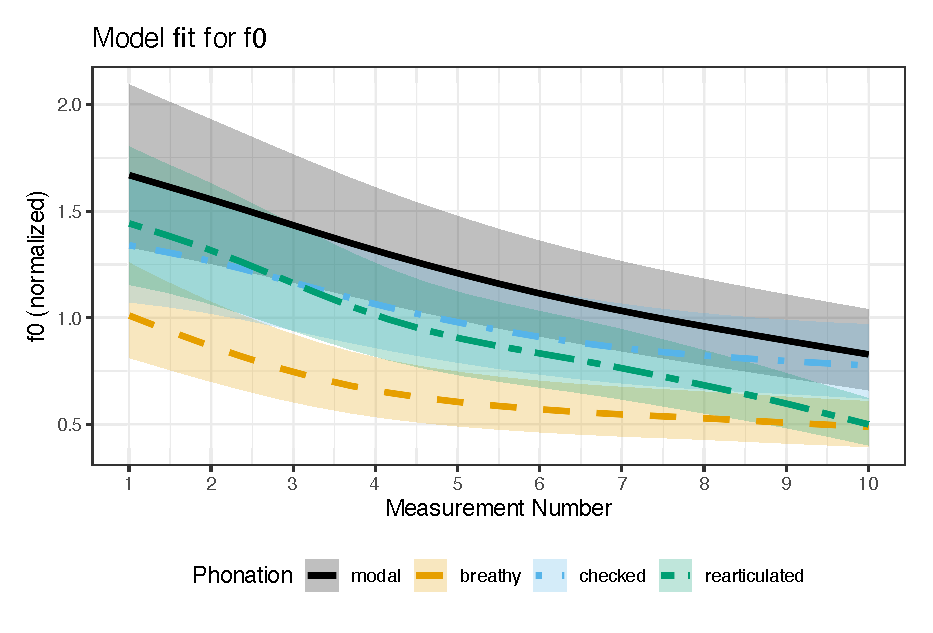
\includegraphics[width = \linewidth]{images/LCH_GAMMs/f0_model_fit.eps}
    \caption{Model fit for \textit{f}0. Each line represents the predicted values from the GAMM for each of the phonations over time. The shaded area represents the 95\% confidence interval.}
    \label{fig:f0_model_fit}
\end{figure}

The observations from the model fit are only part of the story when evaluating GAMMs. The other piece of evidence that we need is whether or not the differences that we observe in the model fit are significant. This is done through difference plots that compare the values for a given comparison (in this case modal versus one of the non-modal phonations) and returns whether or not the difference is significant or not. In these plots, the red line indicates that the difference that we observe between modal and the other phonation types is significant. The blue line indicates that the difference between modal and the non-modal phonation is not significant. This method of evaluation is the most common method for evaluating GAMMs (see \cite{soskuthyEvaluatingGeneralisedAdditive2021} for discussion about evaluating GAMMs). 

Figure~\ref{fig:f0_model_diff} shows the corresponding difference plot for \textit{f}0. The leftmost panel shows the difference plot between modal and breathy voice. The red line indicates that the differences we observed between modal and breathy voice in Figure~\ref{fig:f0_model_fit} is significant across the entire length of the vowel. The center panel shows the differences between modal and checked voice is not significant at any point during the vowel and in terms of \textit{f}0 there is no difference between these two phonations. The rightmost panel shows the difference between modal and rearticulated voice is also not significant for the first part of the vowel. However, beginning at about measurement number 7, we see that the differences are significant.

\begin{figure}[h!]
    \centering
    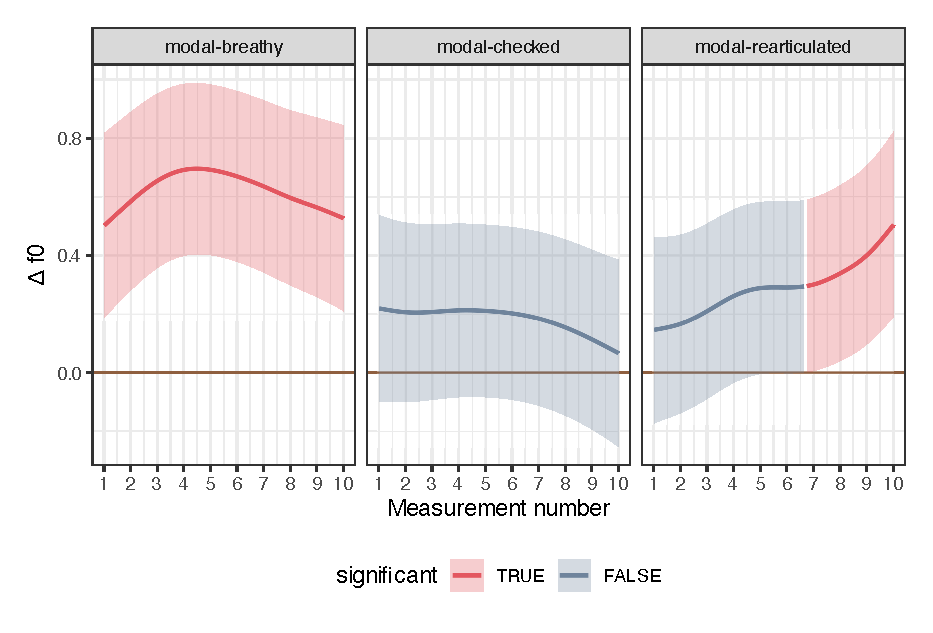
\includegraphics[width = \linewidth]{images/LCH_GAMMs/f0_model_diff.eps}
    \caption{Plot of the difference between modal and each of the non-modal phonation types.}
    \label{fig:f0_model_diff}
\end{figure}

This suggests that in terms of \textit{f}0, breathy voice is significantly different from modal voice throughout the entire duration of the vowel. This is consistent with descriptions for breathy voice cross-linguistically where one of its acoustic cues is a lower \textit{f}0 than modal vowels \citep[e.g.,][]{hillenbrandAcousticCorrelatesBreathy1996}. Whereas rearticulated vowels are only significantly different from modal vowels for the final third of the vowel. The results suggest that in terms of \textit{f}0 perturbation only rearticulated vowels show phasing. 
%--------------------------------------------------------------------------
\subsection{Harmonic-to-noise ratio} \label{sec:model_hnr}
%--------------------------------------------------------------------------

The model fit for HNR < 1500 Hz is shown in Figure~\ref{fig:hnr_model_fit}. In the model fit, we see that modal voice has the highest predicted values for HNR < 1500 Hz, which is consistent with previous research that has shown that modal voice has a higher HNR than non-modal phonation types \citep[e.g.,][]{blankenshipTimeCourseBreathiness1997,blankenshipTimingNonmodalPhonation2002,dekromCepstrumBasedTechniqueDetermining1993,garellekTimingSequencingCoarticulated2012,garellekPhoneticsVoice2019,gerrattTaxonomyNonmodalPhonation2001}. Additionally we see that the three non-modal phonations are all very similar to each other. Checked vowels, however, shows a dipping at the end of the vowel indicating more noise in the signal. 

\begin{figure}[h!]
    \centering
    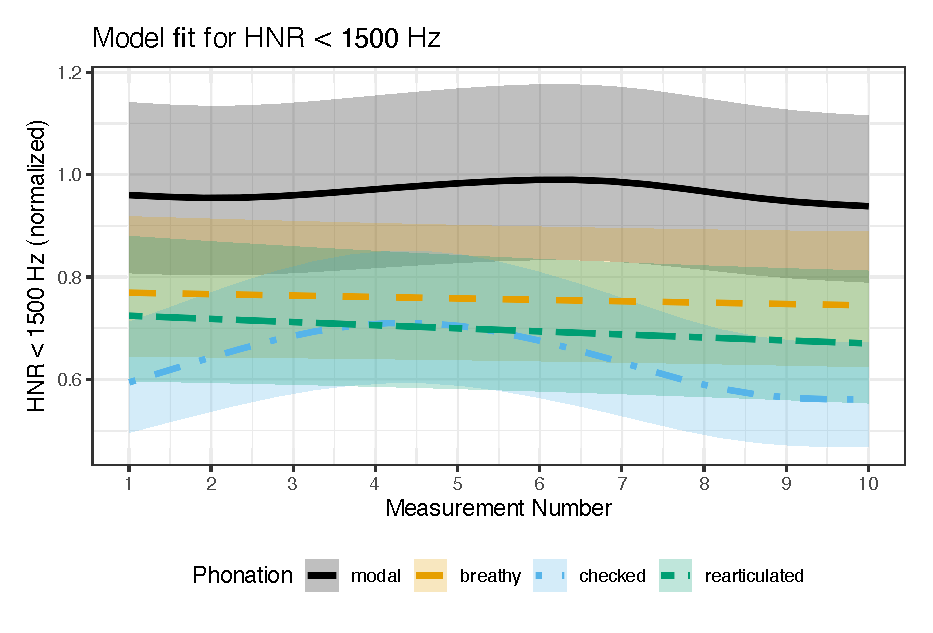
\includegraphics[width = \linewidth]{images/LCH_GAMMs/hnr15_model_fit.eps}
    \caption{Model fit for HNR. Each line represents the predicted values from the GAMM for each of the phonations over time. The shaded area represents the 95\% confidence interval.}
    \label{fig:hnr_model_fit}
\end{figure}  

Figure~\ref{fig:hnr_model_diff} shows the difference plots for each of the non-modal phonations. Similar to Figure~\ref{fig:f0_model_diff}, we see that the leftmost panel shows the difference between modal and breathy voice. This difference is significant from measurement number 4 to halfway between measurements 8 and 9. 

The center and leftmost panels show that the difference between modal and the non-modal phonations is significant across the entire length of the vowel. This indicates that checked and rearticulated vowels are associated with greater aperiodicity across the entire length of the vowel.

\begin{figure}[h!]
    \centering
    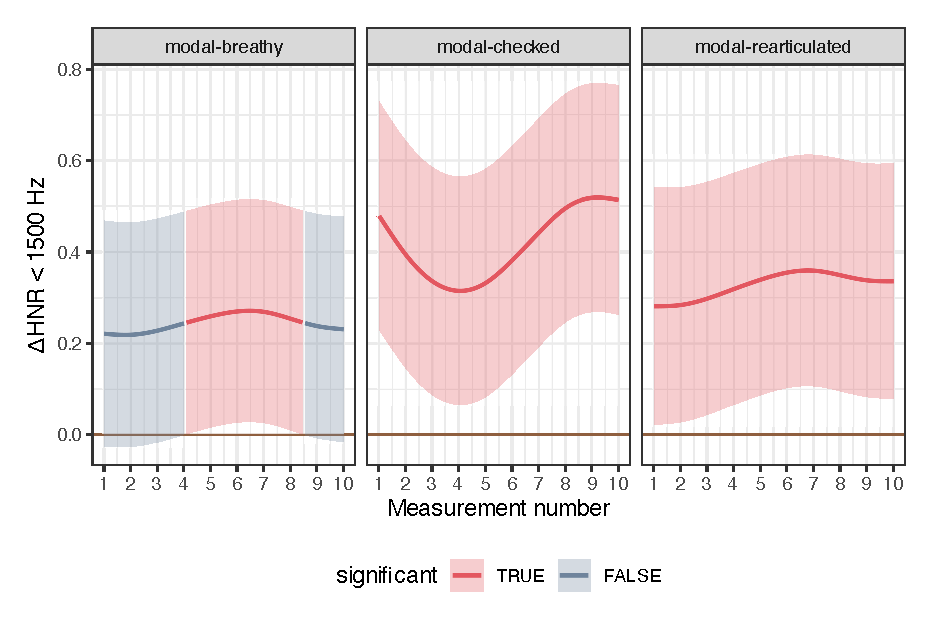
\includegraphics[width = \linewidth]{images/LCH_GAMMs/hnr15_model_diff.eps}
    \caption{Plot of the difference between modal and each of the non-modal phonation types.}
    \label{fig:hnr_model_diff}
\end{figure}

From HNR < 1500 Hz, we see that all three non-modal phonations have more noise in their signal than modal vowels. As I discussed in Section~\ref{sec:bagging_hnr}, HNR measures are typically associated with aperiodicity in the signal. If there is phasing between modal phonation and non-modal phonation as predicted by \citet{silvermanLaryngealComplexityOtomanguean1997}, we would expect to see that these phonations should have a periods where they exhibit more modal-like properties or are not significantly different from modal phonation, which is what we observe with only breathy voice. Breathy vowels show a period of greater aperiodicity than modal vowels in the second half of the vowel, especially if we ignore the interval between 9 and 10 due to coarticulation with the surrounding consonants. Furthermore, this indicates that there is a phasing relationship in breathy vowels where the first half of the vowel is modal and the second half is breathy. 
%--------------------------------------------------------------------------
\subsection{Strength of excitation} \label{sec:model_soe}
%--------------------------------------------------------------------------

As previously discussed in Section~\ref{sec:dt_soe}, SoE is a acoustic measure that correlates to the strength of voicing. Figure~\ref{fig:soe_model_fit} shows the model fit for SoE. In the model fit, we see that modal voice has the highest predicted values for SoE, which is consistent with \citet{garellekVoicingGlottalConsonants2021} where modal vowels are associated with a higher SoE than non-modal phonation because of the greater strength in voicing. 

Breathy voice is identical to modal voice until just after measurement number 2 and then begins to decrease but become identical with modal vowels shortly after measurement number 9. Checked vowels vowels are similar to breathy vowels in that they are identical with modal vowels until just after measurement number 2. However, checked vowels have a sharp decrease in SoE throughout the vowel until measurement number 10. Rearticulated vowels, however, begin lower than the other three phonations but increase in SoE until they are identical with modal voice between measurements 8 and 9. 

\begin{figure}[h!]
    \centering
    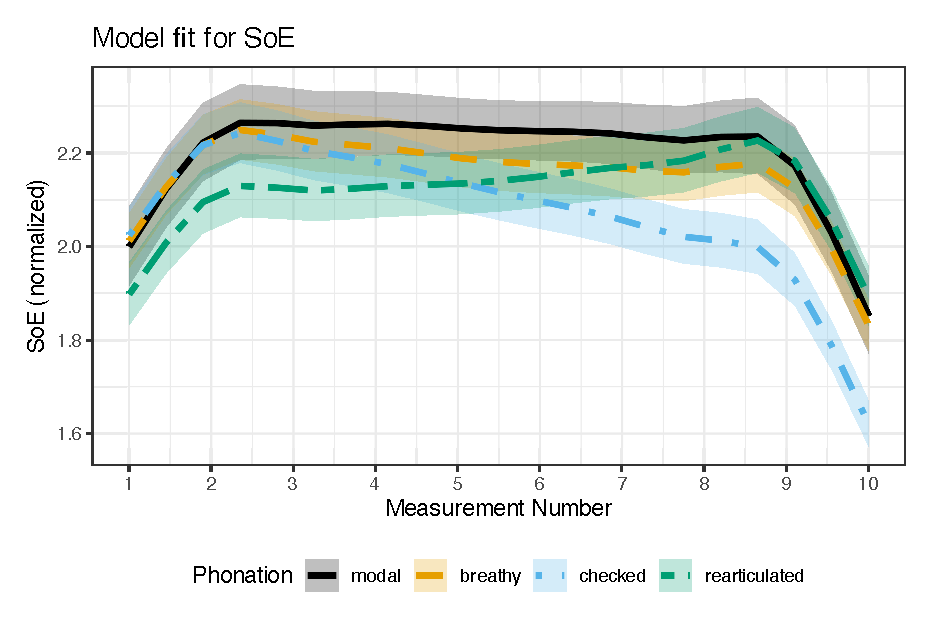
\includegraphics[width = \linewidth]{images/LCH_GAMMs/soe_model_fit.eps}
    \caption{Model fit for SoE. Each line represents the predicted values from the GAMM for each of the phonations over time. The shaded area represents the 95\% confidence interval.}
    \label{fig:soe_model_fit}
\end{figure}

In evaluating whether or not the observed differences from the model fit are significant or not, we can again turn to difference plots to help us determine which differences were significant or not. Figure~\ref{fig:soe_model_diff} shows the difference plots for each of the non-modal phonations. 

The leftmost panel shows the difference between modal and breathy voice. The differences we observed between modal and breathy vowels were only significant between measurement numbers 4 and 8. This is very similar to what we observed in Figure~\ref{fig:hnr_model_diff} for HNR < 1500 Hz. For breathy vowels, we can ignore the interval between measurements 9 and 10 because of the coarticulation with the surrounding consonants.

The center panel shows the difference between modal and checked voice. We observe that checked vowels are significantly different from modal vowels from measurement number 3 to the end of the vowel. However, we can consider the interval between measurements 9 and 10 because checked vowels have a phontactic restriction in the nominal domain that prevents them from occurring in closed syllables. The only time they can accure in a closed syllables is across when a morpheme boundary intervens like in the word \textit{beku'=nh} [bekuˀ=ŋ] `the dog' where the checked vowel occurs across a morpheme boundary.



\begin{figure}[h!]
    \centering
    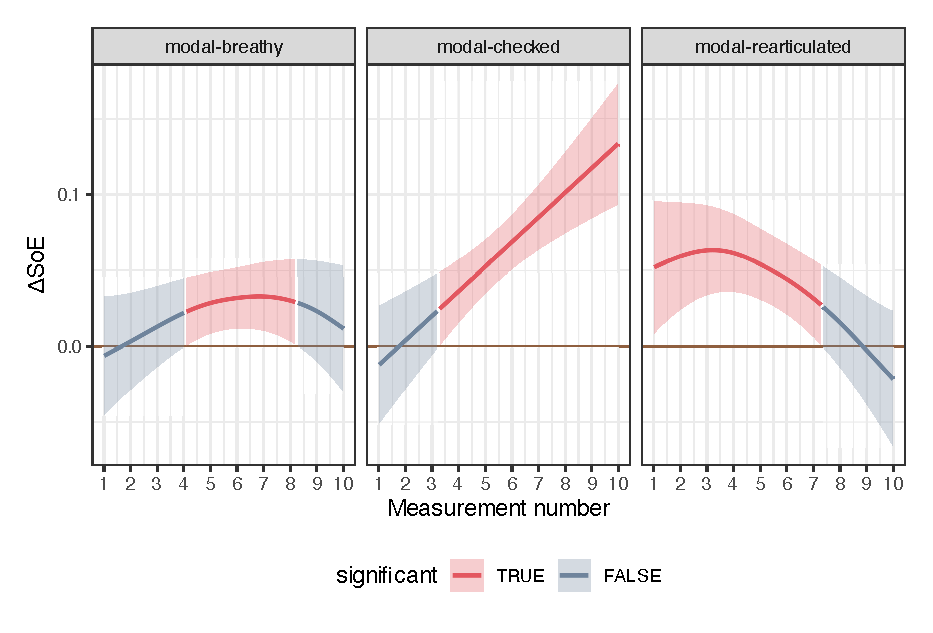
\includegraphics[width = \linewidth]{images/LCH_GAMMs/soe_model_diff.eps}
    \caption{Plot of the difference between modal and each of the non-modal phonation types.}
    \label{fig:soe_model_diff}
\end{figure}


%--------------------------------------------------------------------------
\section{Discussion}\label{sec:discussion_of_lc}
%--------------------------------------------------------------------------

\citet{humbertConsonantTypesVowel1978} 


%--------------------------------------------------------------------------
\section{Conclusion}\label{sec:conclusion_of_lc}
%--------------------------------------------------------------------------

% %--------------------------------------------------------------------------
% Modeling laryngeal complexity
\chapter{Modeling laryngeal complexity} \label{ch:modeling_lc}
%--------------------------------------------------------------------------

%--------------------------------------------------------------------------
\section{The Laryngeal Articulator Model}\label{sec:lam}
%--------------------------------------------------------------------------

\citet{eslingThereAreNo2005,eslingVoiceQualityLaryngeal2019,moisikPhonologicalPotentialsLower2021,moisikMultimodalImagingGlottal2015,moisikModelingBiomechanicalInfluence2014}

\begin{figure}
    \centering
    \begin{tikzpicture}
        \node[draw,circle,minimum size=1cm,inner sep=0pt] (tra) at (0,0) {tra};
        \node[draw,circle,minimum size=1cm,inner sep=0pt] (tfr) at (-2,-1.5) {tfr};
        \node[draw,circle,minimum size=1cm,inner sep=0pt] (tre) at (2,-1.5) {tre};
        \node[draw,circle,minimum size=1cm,inner sep=0pt] (tdb) at (0,-3) {tdb};

        \node[draw,circle,minimum size=1cm,inner sep=0pt] (epc) at (0,-6) {epc};
        \node[draw,circle,minimum size=1cm,inner sep=0pt] (vfo) at (-2,-7.5) {vfo};
        \node[draw,circle,minimum size=1cm,inner sep=0pt] (vfc) at (2,-7.5) {vfc};
        \node[draw,circle,minimum size=1cm,inner sep=0pt] (epv) at (0,-9) {epv};

        \node[draw,circle,minimum size=1cm,inner sep=0pt] (lower_lx) at (-3.5,-6) {↓lx};
        \node[draw,circle,minimum size=1cm,inner sep=0pt] (raised_lx) at (3.5,-6) {↑lx};

        \node[draw,circle,minimum size=1cm,inner sep=0pt] (Lf0) at (-2,-10.5) {Lf0};
        \node[draw,circle,minimum size=1cm,inner sep=0pt] (Hf0) at (2,-10.5) {Hf0};
        
        % Anti-syngeristic
        \draw[<->, dotted, line width=.5mm] (tra.west) to[out=180,in=90] (tfr.north);
        \draw[<->,dotted, line width=.5mm] (tra.east) to[out=0,in=90] (tre.north);
        \draw[<->,dotted, line width=.5mm] (tfr.east) to (tre.west);
        \draw[<->,dotted, line width=.5mm] (tra.south) to (tdb.north);
        \draw[<->,dotted, line width=.5mm] (tfr.south) to[in=180, out=-90] (epc.west);
        \draw[<->,dotted, line width=.5mm] (lower_lx.north) to[in=140,out=40] (raised_lx.north);
        \draw[<->,dotted, line width=.5mm] (lower_lx.east) to (epc.west);
        \draw[<->,dotted, line width=.5mm] (epc.west) to[in=90,out=180] (vfo.north);
        \draw[<->,dotted, line width=.5mm] (vfo.east) to[in=180,out=0] (vfc.west);
        \draw[<->,dotted, line width=.5mm] (vfc.south) to[in=0,out=-90] (epv.east);
        \draw[<->,dotted, line width=.5mm] (epc.south) to[out=-90, in=90] (Hf0.north);
        \draw[<->,dotted, line width=.5mm] (Hf0.south) to[out=-140, in=-40] (Lf0.south);
        \draw[<->,dotted, line width=.5mm] (epv.south) to[out=-90, in=180] (Hf0.west);

        % Syngeristic
        \draw[<->, line width=.5mm] (tdb.west) to[out=180, in=-90] (tfr.south);
        \draw[<->, line width=.5mm] (tdb.east) to[out=0, in=-90] (tre.south);
        \draw[<->, line width=.5mm] (epc.north) to (tdb.south);
        \draw[<->, line width=.5mm] (epc.south) to (epv.north);
        \draw[<->, line width=.5mm] (epc.east) to[in=-90, out=0] (tre.south);
        \draw[<->, line width=.5mm] (lower_lx.north) to[in=-135, out=90] (tfr.west);
        \draw[<->, line width=.5mm] (raised_lx.north) to[in=-45, out=90] (tre.east);
        \draw[<->, line width=.5mm] (Lf0.west) to[in=-90, out =135] (lower_lx.south);
        \draw[<->, line width=.5mm] (raised_lx.west) to (epc.east);
        \draw[<->, line width=.5mm] (Hf0.east) to[in=-90, out=45] (raised_lx.south);
        \draw[<->, line width=.5mm] (epv.south) to[out=-90, in=0] (Lf0.east);
        \draw[<->, line width=.5mm] (epc.east) to[out=0, in=90] (vfc.north);
        \draw[<->, line width=.5mm] (vfo.south) to[out=-90, in=180] (epv.west);
        \draw[<->, line width=.5mm] (vfc.south) to (Hf0.north);
        \draw[<->, line width=.5mm] (vfo.south) to (Lf0.north);
        \draw[<->, line width=.5mm] (epc.south) to[out=-90,in=90] (Lf0.north);
        \draw[<->, line width=.5mm] (lower_lx.south) to[out=-90,in=180] (vfo.west);
        \draw[<->, line width=.5mm] (raised_lx.south) to[out=-90,in=0] (vfc.east);

        % Curly bracket with text
        \draw[decorate,decoration={brace,amplitude=10pt,raise=5pt},thick] (4,0) -- (4,-4) node[midway,xshift=15pt,right=5pt] {\parbox{2cm}{vowel\\quality}};
        \draw[decorate,decoration={brace,amplitude=10pt,raise=5pt},thick] (4,-4) -- (4,-9.5) node[midway,xshift=15pt,right=5pt] {\parbox{2cm}{phonatory\\quality}};
        \draw[decorate,decoration={brace,amplitude=10pt,raise=5pt},thick] (4,-9.5) -- (4,-11) node[midway,xshift=15pt,right=5pt] {\parbox{2cm}{tonal\\quality}};
        \draw[decorate,decoration={brace,amplitude=10pt,raise=5pt},thick] (7,-2) -- (7,-11) node[midway,xshift=15pt,right=5pt] {\parbox{2cm}{voice\\quality}};

        
    \end{tikzpicture}
    \caption{The Laryngeal Articulator Model from \citet{eslingVoiceQualityLaryngeal2019}. This model shows the interactions between the laryngeal articulators (labeled circles). Syngeristic interactions are shown with solid lines, while anti-syngeristic interactions are shown with dotted lines.}
    \label{fig:tra}
\end{figure}

%--------------------------------------------------------------------------
\section{Modeling laryngeal complexity}\label{sec:modeling_lc}
%--------------------------------------------------------------------------

%--------------------------------------------------------------------------
\section{Alternative accounts}\label{sec:alternative_accounts}
%--------------------------------------------------------------------------

%--------------------------------------------------------------------------
\subsection{Articulatory Phonology account}\label{sec:ap_account}
%--------------------------------------------------------------------------

%--------------------------------------------------------------------------
\subsection{Q-theory account}\label{sec:q_theory_account}
%--------------------------------------------------------------------------

%--------------------------------------------------------------------------
\subsection{Radical CV Phonology account}\label{sec:rcv_account}
%--------------------------------------------------------------------------

%--------------------------------------------------------------------------
\section{Conclusion}\label{sec:conclusion_of_modeling_lc}
%--------------------------------------------------------------------------
\chapter{Conclusion}

%--------------------------------------------------------------------------
%  Bibliography
%--------------------------------------------------------------------------
% LTeX: enabled=false
%%-----------------------------------------
%% Bibliography 
%%-----------------------------------------
%%% Not that I use amsrefs
% \clearpage
\phantomsection
	%\bibliography{Thesis.bib}
\begin{bibdiv}
	\addchaptertocentry{}{Bibliography}% Add bib title to toc
\begin{biblist}

%Put your bib entires here.

\end{biblist}
\end{bibdiv}
% N.B. by default I use raw amsrefs. If you prefer to let amsrefs load .bib file, use the following instead:
%\bibliography{yourbibfile}

% \appendix
% %Appendix chapter
\chapter{Wordlist}

\begin{longtable}{lllll}
\lsptoprule
 Lexeme & Eng. Gloss & Sp. Gloss & Phonation   & Tone   \\
\midrule
 \textit{xa'ag}  & sheriff, police    & \textit{topíl} & R & L \\
 \textit{xmanh}  & week  & \textit{semana}    & M & HL \\
 \textit{xche}   & dinner & \textit{cena} & M & H \\
 \textit{yu'u}   & house & \textit{casa}  & R & HL    \\
 \textit{rmedzw} & remedy    & \textit{remedio}   & M & H \\
 \textit{yu'}    & earth & \textit{tierra}    & C & L \\
 \textit{za'a}   & corncob   & \textit{elote} & R & HL \\
 \textit{behl}   & snake & \textit{vibora}    & B & L \\
 \textit{tsil}   & in the morning    & \textit{en la mañana} & M & HL \\
 \textit{bel}    & fish & \textit{pez} & M & HL \\
 \textit{bzine'} & rat; mouse & \textit{ratón} & MC & LL \\
 \textit{bedzjw} & turkey    & \textit{guajolote} & M & H \\
 \textit{rbej}   & pea   & \textit{chícharo}  & M & L \\
 \textit{behb}   & trash & \textit{basura}    & B & L \\
 \textit{bene'}  & person & \textit{persona} & MC & MH \\
 \textit{yich}   & paper & \textit{papel} & M & L \\
 \textit{dam}    & owl & \textit{tecolote/buho} & M & H \\
 \textit{blull}  & frog; toad & \textit{sapo; rana} & M & L \\
 \textit{yag}    & measure of corn   & \textit{almúd} & M & L \\
 \textit{bgah}   & necklace; bracelet & \textit{collar} & B & L \\
 \textit{behlhe'} & meat & \textit{carne} & BC & LL \\
 \textit{lni}    & party & \textit{fiesta} & M & L \\
 \textit{jid}    & chicken & \textit{gallina} & M & MH \\
 \textit{bdze'}  & ant & \textit{hormiga} & C & L \\
 \textit{yichbahlh} & midnight & \textit{madrugada/medianoche}  & B & LHL    \\
 \textit{chi'im (bi'a ser)} & honey & \textit{miel de abeja} & R & H \\
 \textit{ya'a}   & market & \textit{mercado} & R & L \\
 \textit{llume}  & basket & \textit{canasta} & MM & MH \\
 \textit{xwe}    & lunch & \textit{comida} & M & L \\
 \textit{xsil}   & breakfast & \textit{almuerzo} & M & L \\
 \textit{yell}   & village & \textit{pueblo} & M & HL \\
 \textit{behche'} & wasp's nest & \textit{panal/nido de avispas} & BC & LL \\
 \textit{yej}    & flower & \textit{flor} & M & L \\
 \textit{shchag} & noise & \textit{ruido} & M & HL \\
 \textit{deh}    & ash & \textit{ceniza} & B & L \\
 \textit{bxhillu'} & badger; coati & \textit{tejón} & MC & HL \\
 \textit{kampanh} & bell & \textit{campana} & MM & MHL    \\
 \textit{cha'}   & cooking pot & \textit{cazuela} & C & L \\
 \textit{lhe'ej} & fence; corral & \textit{cerca; jaripeo} & R & HL \\
 \textit{chib}   & goat & \textit{chivo} & M & HL \\
 \textit{xhidw}  & cat & \textit{gato} & MW & MH \\
 \textit{bo'}    & coal & \textit{carbón} & C & L \\
 \textit{bsuh}   & adobe & \textit{adobe} & B & HL \\
 \textit{ze'e}   & wall & \textit{pared} & RR & HL \\
 \textit{pantlon} & pants & \textit{pantalones} & MM & MHL \\
 \textit{sukr}   & sugar & \textit{azucar} & M & H \\
 \textit{gwanhax} & garlic & \textit{ajo} & MM & LHL \\
 \textit{iz}     & year & \textit{año} & M & L \\
 \textit{bxhidw} & kiss & \textit{beso} & M & M \\
 \textit{yitw}   & pumpkin & \textit{calabaza} & M & HL \\
 \textit{beht}   & skunk & \textit{zorrillo} & B & L \\
 \textit{yah}    & iron; rifle & \textit{fierro; rifle} & B & L \\
 \textit{pyine}  & bird & \textit{pájaro} & MM & MM \\
 \textit{yet}    & tortilla & \textit{tortilla} & M & L \\
 \textit{lok}    & angry & \textit{enojado} & M & L \\
 \textit{biu'walh} & full moon & \textit{luna llena} & M & H \\
 \textit{zix}    & sweet & \textit{dulce} & M & H \\
 \textit{shlkan/kandadw} & lock & \textit{candado} & MM & MH \\
 \textit{player} & t-shirt & \textit{playera} & MM & MH \\
 \textit{botey}  & bottle  & \textit{botella} & MM & MH \\
 \textit{duh}    & rope; cord & \textit{mecate; cuerda} & B & L \\
 \textit{da'abep}    & reed & \textit{capisallo} & RM & L \\
 \textit{yi'inh} & chili pepper & \textit{chile} & R & L \\
 \textit{blli'in} & beast of burden; mule & \textit{bestia; mulo} & R & HL \\
 \textit{zahg} & cold & \textit{frío} & B & L \\
 \textit{zah}    & bean & \textit{frijol} & B & L \\
 \textit{xkalh}  & mayor & \textit{alcalde} & M & L \\
 \textit{xtilh}  & white & \textit{blanco}  & M & HL \\
 \textit{chich}  & white & \textit{blanco} & M & H      \\
 \textit{libr}   & book & \textit{libro} & M & H \\
 \textit{yag}    & tree; wood & \textit{árbol} & M & L \\
\lspbottomrule
\end{longtable}


\end{document}
